 \documentclass[12pt,twoside]{report}

% note that the document can be single or double sided.

%\usepackage{uicthesis}
\usepackage{uicthesis2}      % the style of 'uicthesis2' includes the list of tables and figues, choose it by yourself.
\usepackage{graphicx,overpic}
\usepackage{amsmath,amssymb}

\newtheorem{theorem}{Theorem} [chapter]
\newtheorem{lemma}{Lemma}[chapter]
\newtheorem{coro}{Corollary}[chapter]
\newtheorem{defi}{Definition}[chapter]
\newtheorem{example}{Example}[chapter]
\def\proof {\noindent{\bf Proof.}\quad}



\newcommand{\ba}{\begin{array}}
\newcommand{\ea}{\end{array}}
\newcommand{\bt}{\begin{tabular}}
\newcommand{\et}{\end{tabular}}
\newcommand{\btb}{\begin{table}}
\newcommand{\etb}{\end{table}}
\newcommand{\bc}{\begin{center}}
\newcommand{\ec}{\end{center}}
\newcommand{\bea}{\begin{eqnarray}}
\newcommand{\eea}{\end{eqnarray}}
\newcommand{\Bea}{\begin{eqnarray*}}
\newcommand{\Eea}{\end{eqnarray*}}
\newcommand{\beq}{\begin{equation}}
\newcommand{\eeq}{\end{equation}}


\def \bfm#1{\mbox{\boldmath$#1$}}
%\def \bfm#1{\mathbf{#1}}

\def \A {{\bfm A}} \def \a {{\bfm a}}  \def \b {{\bfm b}}
\def \B {{\bfm B}} \def \c {{\bfm c}} \def \C {{\bfm C}}
\def \d {{\bfm d}} \def \D {{\bfm D}} \def \e {{\bfm e}}
\def \E {{\bfm E}}
\def \f {{\bfm f}} \def \G {{\bfm G}} \def \g {{\bfm g}}
\def \h {{\bfm h}} \def \H {{\bfm H}} \def \K {{\bfm K}}
\def \I {{\bfm I}} \def \m {{\bfm m}} \def \M {{\bfm M}}
\def \N {{\bfm N}} \def \o {{\bfm o}} \def \p {{\bfm p}}
\def \P {{\bfm P}} \def \r {{\bfm r}} \def \R {{\bfm R}}
\def \s {{\bfm s}} \def \S {{\bfm S}}
\def \t {{\bfm t}} \def \u {{\bfm u}} \def \U {{\bfm U}}
\def \w {{\bfm w}} \def \W {{\bfm W}} \def \v {{\bfm v}}

\def \X {{\bfm X}} \def \x {{\bfm x}}
\def \Y {{\bfm Y}} \def \y {{\bfm y}}
\def \Z {{\bfm Z}} \def \z {{\bfm z}}
\def \eps {\varepsilon} \def \Eps {\bfm \varepsilon}

\def \th {{\bfm \theta}}
\def \one {{\bf 1}}\def \zero {{\bf 0}}
\def \Tau {{\bfm \tau}} \def \Alpha {{\bfm \alpha}}
\def \Beta {{\bfm \beta}}
\def \var {\mbox{Var}} \def \cov {\mbox{Cov}}
\def \tr {\mbox{tr}}

%\def \tX {{\tilde {\bfm X}}} \def \tx {{\tilde{\bfm x}}}
\def \tX {\mbox{\textbf{X}}}


\def \ca {{\mathcal A}}
\def \cb {{\mathcal B}} \def \cd {{\mathcal D}}
\def \cw {{\mathcal W}} \def \ck {{\mathcal K}}
\def \cx {{\mathcal X}} \def \cm {{\mathcal M}} \def \cn {{\mathcal N}}
\def \cl {{\mathcal L}} \def \cR {{\mathcal R}}
\def \cu {{\mathcal U}} \def \ch {{\mathcal H}} \def \cp {{\mathcal P}}


\begin{document}

    \title{Timing Synchronization for Orthogonal
    Frequency-Division Multiplexing Systems}

    \author{Zhuoyang Zhou}
    \studentid{2330005071}
    \credit{STAT4004}
    \dept{Statistics}
    \submitdate{December, 2026}

    \beforepreface


% Abstract and keywords; heading structure follows the thesis template.
\begin{center}
{\Large\sffamily\bfseries Timing Synchronization for Orthogonal\\
Frequency-Division Multiplexing Systems\par}
\vspace{2mm}
{\large Zhuoyang Zhou\par}
\vspace{2mm}
{\large Statistics\par}
\vspace{2mm}
{\Large\bfseries Abstract\par}
\end{center}

This study compares four representative preamble-based timing estimators for orthogonal frequency-division multiplexing (OFDM): Schmidl--Cox (S\&C), Park-type, Minn-type and CAZAC-based (constant-amplitude zero-autocorrelation) methods. Two MATLAB Monte Carlo experiments each evaluate 880,000 estimates in additive white Gaussian noise (AWGN) and fixed multipath at signal-to-noise ratios of 0--20~dB. With equal training duration and energy, metrics include timing mean squared error (MSE), exact and cyclic prefix (CP) safety probabilities, and bit error rate (BER).

CAZAC achieves 219,997 exact estimates out of 220,000 with a known template. At 20~dB AWGN, S\&C achieves CP-safe and exact probabilities of 0.9978 and 0.0006; squared bias accounts for 97.36\% of its MSE. Park and Minn still exhibit occasional large errors. In the separate BER experiment at 20~dB AWGN, oracle phase correction using true timing error reduces S\&C bit errors from 639,428 to one out of 1,280,000 bits. Exact timing, CP-safe placement and reliable detection are thus distinct objectives.

\vspace{2mm}
\noindent\textbf{Keywords}: OFDM, timing synchronization, Monte Carlo simulation, mean squared error, cyclic prefix, bit error rate.


%\chapter*{Preface}


This thesis tells you all you need to know about life, the universe,
and everything.

\newpage

However everything should be taken with a grain of salt.


\chapter*{Acknowledgement}

I would like to express my sincere gratitude to my supervisor, Dr. Xinwei Du, for his guidance, constructive feedback and support throughout this Final Year Project. His advice on the timing synchronization methods, simulation design and interpretation of the experimental results helped me develop a clearer understanding of the research problem and improve the rigor of this study.

I also appreciate the opportunity to apply the statistical methods learned during my undergraduate studies to a problem in digital communications. Completing this project has deepened my understanding of Monte Carlo simulation, quantitative performance evaluation and the importance of reproducible research.

Finally, I would like to thank everyone who has supported me during the completion of this project.


\afterpreface

% Chapter 1: Introduction
\chapter{Introduction}
\label{chap:introduction}

\section{Research Background}
Orthogonal frequency-division multiplexing (OFDM) divides a broadband data stream among mutually orthogonal subcarriers. The inverse fast Fourier transform (IFFT) generates the time-domain signal at the transmitter, and the fast Fourier transform (FFT) recovers the subcarrier symbols at the receiver. With a sufficiently long cyclic prefix (CP) and appropriate receiver timing, a frequency-selective channel can be represented by a separate complex gain on each subcarrier, simplifying equalization \cite{vannee2000,morelli2007}.

These advantages depend on synchronization. Before applying the FFT, the receiver must locate the useful portion of the received OFDM symbol. An incorrectly positioned FFT window can introduce a subcarrier-dependent phase rotation even when it remains within a region protected by the CP. When the window extends beyond this region, inter-symbol interference (ISI) and inter-carrier interference (ICI) may arise. The resulting degradation depends not only on the magnitude of the timing error but also on its direction, the channel impulse response, and the receiver's compensation strategy.

Preamble-based timing synchronization exploits a training symbol transmitted before the data. The Schmidl--Cox (S\&C) method uses two repeated time-domain halves to form a correlation metric; the CP can produce a plateau that makes the exact symbol boundary ambiguous \cite{schmidl1997}. Park et al. proposed a training and correlation structure intended to produce a sharper timing peak \cite{park2003}. Minn et al. investigated training designs with a steeper timing-metric roll-off \cite{minn2003}. Constant-amplitude zero-autocorrelation (CAZAC) sequences offer another approach through their favorable correlation properties \cite{fang2012}. These studies motivate a comparison of timing estimators that use different training structures and decision rules.

The timing metric alone does not characterize the statistical reliability of an estimator. A narrow peak in one received frame does not establish a high probability of correct timing across repeated noisy observations. Likewise, a low exact-timing probability need not imply that most FFT windows are outside the CP-safe region. A comparison based on repeated trials is therefore needed to distinguish systematic estimation bias, random variation, and occasional large errors. The effect of these errors on the complete OFDM receiver must also be examined separately.

\section{Problem Statement}
\label{sec:problem-statement}
The central research problem, as defined in the project proposal, is how different preamble-based digital signal processing (DSP) timing synchronization algorithms for an OFDM receiver compare in timing accuracy and end-to-end detection performance under noise and multipath channels.

This problem has two related levels. At the estimator level, the receiver must select a timing position from a set of candidate positions in the presence of additive white Gaussian noise (AWGN) and channel dispersion. The mean squared error (MSE) measures the average squared displacement from the reference position, but it does not distinguish a persistent small bias from a small number of large errors. Correct timing-estimation probability complements MSE by measuring the frequency with which a specified timing criterion is satisfied. In this study, exact timing and CP-safe timing are reported separately to distinguish precise boundary identification from operationally acceptable window placement.

At the system level, the estimated timing position determines the FFT window used for data recovery. Even a CP-safe estimate may cause a deterministic phase rotation across subcarriers, leading to detection errors if the rotation is not compensated. Accordingly, timing accuracy and bit error rate (BER) are related but are not interchangeable measures of receiver performance. This study uses timing MSE and correct estimation probability as the principal measures, with BER as a supplementary end-to-end measure.

\section{Research Questions and Objectives}
\subsection{Research Questions}
The four research questions follow the approved project proposal:
\begin{enumerate}
\item[\textbf{RQ1.}] How does timing offset affect the received OFDM signal and BER when synchronization is absent or inaccurate?
\item[\textbf{RQ2.}] How do the Schmidl--Cox, Park, Minn and CAZAC-based timing synchronization methods differ in timing-metric behavior, timing-estimation MSE and correct estimation probability?
\item[\textbf{RQ3.}] How does synchronization performance change with SNR and representative impairments, including multipath/channel dispersion and, where feasible, carrier-frequency offset (CFO) and phase noise?
\item[\textbf{RQ4.}] How do improvements in timing-estimation accuracy relate to end-to-end OFDM detection performance, as measured by BER?
\end{enumerate}
The completed experimental investigation addresses the core timing-synchronization questions under AWGN and a fixed multipath channel. CFO and phase noise were optional extensions in the proposal and are not evaluated in this study.

\subsection{Research Objectives}
The overall objective is to study and compare OFDM timing synchronization algorithms using a reproducible MATLAB simulation platform. The specific objectives are:
\begin{enumerate}
\item To construct and verify a complex-baseband OFDM transmitter and receiver, including modulation, subcarrier mapping, IFFT/FFT processing, CP insertion and removal, channel transmission, and symbol detection.
\item To model controlled positive and negative timing offsets and examine their effects on demodulation and detection.
\item To implement and compare four representative preamble-based methods: Schmidl--Cox, Park-type, Minn-type, and CAZAC-based synchronization.
\item To evaluate timing MSE and correct estimation probability across SNR and channel conditions, supported by empirical timing-error distributions.
\item To evaluate BER as a supplementary system-level measure and discuss robustness and approximate computational complexity.
\item To investigate tolerance to representative multipath dispersion and identify the limitations of the completed experiments, including the optional CFO and phase-noise extensions not undertaken.
\end{enumerate}

\section{Scope of the Study}
The investigation is restricted to simulated complex-baseband OFDM with quadrature phase-shift keying (QPSK), 64 subcarriers, and a CP of 16 samples. The formal comparative experiments use one CP-inclusive training symbol and one data symbol per frame, each of length 80 samples and normalized to the same energy. Integer-sample arrival delays are considered. The channel conditions comprise AWGN and a deterministic three-tap multipath channel with AWGN added after convolution; the latter is not an ensemble of random fading channels.

The four estimators are representative implementations rather than a claim of exact reproduction of every published algorithm. The Park-type implementation uses the training and metric confirmed by the project supervisor, the Minn-type method uses a time-domain Golay-based training structure, and the CAZAC-based method uses a known Zadoff--Chu preamble with normalized matched correlation. The methods share training duration, energy, timing reference, and candidate search interval in the formal comparison, but their receiver-side knowledge and decision rules differ. In particular, the CAZAC-based estimator uses the complete known training template. These distinctions limit the interpretation of comparative performance.

The end-to-end BER experiment compares perfect timing, estimated timing, and estimated timing with oracle phase compensation. The physical channel response is assumed known for equalization. The oracle additionally uses the true timing error and is a diagnostic reference rather than a practical estimation or compensation method. Fractional-sample timing offsets, CFO, phase noise, random fading profiles, and practical channel estimation are outside the completed experimental scope.

\section{Research Contributions}
The contribution is a controlled, reproducible, quantitatively supported comparison rather than a new state-of-the-art synchronization algorithm. The study establishes a modular OFDM simulation framework and verifies its baseline behavior before introducing timing offsets and synchronization estimators. This progressive design separates basic transmitter and receiver validation from the effects of timing estimation.

A unified Monte Carlo experiment compares the four selected implementations using common arrival-delay scenarios, data symbols, underlying noise realizations, and channel models. Each algorithm is evaluated at 11 SNR values under two channel conditions, with 10,000 trials per condition. Reporting exact timing probability, CP-safe timing probability, and timing MSE separately provides a basis for interpreting differences in estimation bias and error magnitude.

The study further connects estimator-level performance with system-level detection by placing the FFT window according to the estimated timing position. The comparison with perfect timing and oracle phase compensation helps distinguish degradation attributable to residual phase rotation from degradation that remains when the FFT window is outside the safe region. This links the statistical properties of timing estimators to the practical consequences of their errors under the specified receiver assumptions.

\section{Thesis Organization}
Chapter~2 reviews the literature and introduces the theoretical background of OFDM, timing offsets, and preamble-based synchronization. Chapter~3 describes the simulation framework, actual estimator implementations, channel assumptions, Monte Carlo design, evaluation metrics, and receiver configurations. Chapter~4 presents baseline verification, timing-offset sensitivity, individual estimator validation, and the unified statistical comparison of timing performance. Chapter~5 examines end-to-end BER, the relationship between timing errors and detection performance, approximate computational complexity, and the limitations of the comparison. Chapter~6 summarizes the findings and identifies directions for future work.


% Chapter 2: Literature Review and Theory
\chapter[Literature Review and Theory]
{Literature Review and Theoretical Background}
\label{chap:theory}

\section{Fundamentals of OFDM}
Orthogonal frequency-division multiplexing represents a wideband transmission as a collection of narrowband subcarrier signals. The subcarriers overlap in frequency but remain orthogonal over the useful symbol duration. This permits efficient use of bandwidth and, with an appropriate guard interval, simplifies equalization in frequency-selective channels \cite{vannee2000,morelli2007}.

Let $N$ denote the number of subcarriers and $X[k]$ the complex modulation symbol on subcarrier $k$. Using the discrete Fourier transform (DFT) convention of MATLAB, the useful time-domain symbol is
\begin{equation}
 x[n]=\frac{1}{N}\sum_{k=0}^{N-1}X[k]\exp(j2\pi kn/N),\qquad 0\leq n<N.
 \label{eq:ofdm_ifft}
\end{equation}
The corresponding receiver transform is
\begin{equation}
 X[k]=\sum_{n=0}^{N-1}x[n]\exp(-j2\pi kn/N).
 \label{eq:ofdm_fft}
\end{equation}
Here $j=\sqrt{-1}$. The normalization differs from the unitary DFT convention, which uses $1/\sqrt{N}$ in both directions. The two conventions describe the same transform pair up to a known scaling factor; transmitted power and receiver scaling must be handled consistently.

Orthogonality follows from the finite geometric sum
\begin{equation}
 \frac{1}{N}\sum_{n=0}^{N-1}\exp(j2\pi(k-m)n/N)
 =\begin{cases}1,&k=m,\\0,&k\ne m,\end{cases}
 \label{eq:orthogonality}
\end{equation}
for $k,m\in\{0,\ldots,N-1\}$. Substituting (\ref{eq:ofdm_ifft}) into (\ref{eq:ofdm_fft}) therefore recovers each transmitted symbol without contributions from the other subcarriers in an ideal channel.

Quadrature phase-shift keying (QPSK) conveys two bits per complex symbol. A unit-energy constellation can be expressed as $\exp(j(\pi/4+q\pi/2))$, where $q\in\{0,1,2,3\}$. This relatively simple modulation permits the effects of synchronization to be examined without introducing higher-order modulation or channel coding. For coherent Gray-coded QPSK in AWGN with perfect synchronization, the theoretical bit error probability \cite{proakis2008} is
\begin{equation}
 P_b=Q\left(\sqrt{2E_b/N_0}\right)
 =\frac{1}{2}\operatorname{erfc}\left(\sqrt{E_b/N_0}\right),
 \label{eq:qpsk_ber}
\end{equation}
where $E_b$ is useful-data energy per bit and $N_0$ is the noise spectral-density parameter. This reference is used for baseline verification, rather than as a theoretical BER expression for an incorrectly synchronized multipath receiver.

\section{Cyclic Prefix and Channel Modeling}
\subsection{Cyclic prefix}
Let $G=N_{\mathrm{CP}}$ denote the cyclic-prefix length. With the useful symbol starting at time index zero, its CP-extended representation is
\begin{equation}
 x_{\mathrm{cp}}[n]=x[n\bmod N],\qquad -G\leq n\leq N-1.
 \label{eq:cp_extension}
\end{equation}
The prefix repeats the final $G$ samples of the useful symbol. Its purpose is not to increase information content but to provide a guard interval that permits circular convolution over the FFT observation window. The fraction of transmitted samples occupied by useful data in a CP-inclusive symbol is $N/(N+G)$, excluding other overhead such as preambles.

\subsection{Discrete-time channel}
Consider a causal, time-invariant channel over one frame, with impulse response $h[\ell]$ for $0\leq\ell\leq L_h-1$. Let $\nu=L_h-1$ be its maximum nonzero delay in samples, measured relative to the first path at delay zero. If $s[n]$ denotes the complete transmitted stream and $\tau$ its integer arrival delay, the received signal is modeled as
\begin{equation}
 r[n]=\sum_{\ell=0}^{\nu}h[\ell]s[n-\tau-\ell]+w[n],
 \label{eq:channel_model}
\end{equation}
where $w[n]$ is zero-mean circular complex Gaussian noise with $\mathbb{E}|w[n]|^2=\sigma_w^2$. Its real and imaginary components are independent with variance $\sigma_w^2/2$. A single-path AWGN model is obtained by setting $h[0]=1$ and $\nu=0$. A multipath channel has additional delayed components and may attenuate or rotate different subcarriers differently.

If $G\geq\nu$ and the FFT window starts at the true useful-symbol boundary, the samples involved in convolution all belong to the same CP-extended symbol. After CP removal, the channel acts as circular convolution. Applying the DFT gives
\begin{equation}
 Y[k]=H[k]X[k]+W[k],\qquad
 H[k]=\sum_{\ell=0}^{\nu}h[\ell]\exp(-j2\pi k\ell/N).
 \label{eq:freq_channel}
\end{equation}
For known nonzero $H[k]$, zero-forcing equalization divides $Y[k]$ by $H[k]$. This simplifies symbol recovery, although small channel gains amplify noise. The model assumes no carrier-frequency offset or phase noise.

\section{Effects of Symbol Timing Offset}
\subsection{Derivation of the CP-safe interval}
Let $d_0$ denote the true received useful-symbol start and $\widehat d$ the estimated start, both measured in the same sample-index convention. Define
\begin{equation}
 e=\widehat d-d_0.
 \label{eq:timing_error}
\end{equation}
Negative errors correspond to early FFT windows and positive errors to late windows. The receiver observes $N$ samples starting at $d_0+e$. Relative to the transmitted useful-symbol boundary, the channel input indices involved are $n+e-\ell$ for $0\leq n<N$ and $0\leq\ell\leq\nu$. Their smallest and largest possible values are $e-\nu$ and $N-1+e$, respectively.

To ensure that all these indices lie within the same CP-extended symbol, it is sufficient to require
\begin{equation}
 e-\nu\geq-G,\qquad N-1+e\leq N-1.
\end{equation}
Combining the inequalities yields the operational CP-safe interval
\begin{equation}
 \boxed{\nu-G\leq e\leq 0.}
 \label{eq:cp_safe}
\end{equation}
For example, with $G=16$, the interval is $[-16,0]$ for a single path and $[-14,0]$ for a channel with maximum delay two samples. The endpoints are inclusive for integer-sample timing. This result assumes a causal channel whose first path is the timing reference and a sufficiently long CP. It is a sufficient condition for avoiding contributions from adjacent symbols under the stated model; it is not a general guarantee of correct detection.

\subsection{Phase rotation within the safe interval}
Inside the interval in (\ref{eq:cp_safe}), the received FFT-window samples can be written as
\begin{equation}
 y_e[n]=\sum_{\ell=0}^{\nu}h[\ell]x[(n+e-\ell)\bmod N]+w_e[n].
\end{equation}
Substituting the inverse DFT expression and collecting terms gives
\begin{equation}
 y_e[n]=\frac{1}{N}\sum_{k=0}^{N-1}X[k]H[k]
 \exp(j2\pi ke/N)\exp(j2\pi kn/N)+w_e[n].
\end{equation}
By orthogonality, its DFT is
\begin{equation}
 \boxed{Y_e[k]=H[k]X[k]\exp(j2\pi ke/N)+W_e[k].}
 \label{eq:timing_phase}
\end{equation}
Thus a CP-safe timing error does not destroy the circular-convolution relationship, but introduces a linear phase progression across subcarrier index $k$. The sign in (\ref{eq:timing_phase}) follows directly from the definition $e=\widehat d-d_0$ and the negative-exponent receiver DFT.

Equalization by the physical channel alone leaves this phase rotation in the detected signal. If $e$ were known, an ideal effective channel could instead be defined as
\begin{equation}
 H_{\mathrm{eff}}[k]=H[k]\exp(j2\pi ke/N).
 \label{eq:effective_channel}
\end{equation}
Dividing by $H_{\mathrm{eff}}[k]$ removes the deterministic rotation. This is the basis of the oracle diagnostic used later in the study. It requires knowledge of the true error and does not represent a deployable synchronization algorithm.

\subsection{Timing outside the safe interval}
When $e<\nu-G$ or $e>0$, some samples in the FFT window may depend on an adjacent symbol or on samples outside the transmitted frame. The circular-convolution model is then generally invalid. Inter-symbol interference and inter-carrier interference may arise, and a phase-only correction cannot in general recover the missing or corrupted samples. Consequently, exact timing, CP-safe timing and BER measure different aspects of performance. The effects of timing and frequency synchronization errors on multicarrier receivers are reviewed more broadly in \cite{morelli2007}.

\section{Preamble-Based Timing Synchronization}
Preamble-based synchronization introduces a training symbol whose structure is selected to facilitate timing acquisition. An alternative is to exploit CP redundancy without additional pilots, as in the joint maximum-likelihood timing and frequency estimator of van de Beek et al. \cite{vandebeek1997}. The present study focuses on preamble-based methods instead. A receiver computes a timing metric $M(d)$ for candidate positions $d$ in a search set $\mathcal{D}$, followed by a decision rule. A common rule is
\begin{equation}
 \widehat d_{\mathrm{raw}}=\arg\max_{d\in\mathcal{D}}M(d),
\end{equation}
although a plateau-based method may use multiple adjacent metric values. The raw metric index may represent a CP boundary, an internal symmetry center or a useful-symbol start. A consistent conversion to the same physical reference is necessary before comparing timing errors.

Correlation-based designs can exploit either relationships among received samples or a known local training sequence. Energy normalization reduces sensitivity to amplitude scaling, but different normalizations have different noise behavior and need not produce metrics bounded by one. Sharp peaks can reduce ambiguity, yet noise, multipath and competing correlation peaks may still cause large errors. The following sections discuss the design principles underlying the four methods selected in the proposal. Exact implementation choices are reserved for Chapter 3.

\section{Schmidl--Cox Synchronization}
Schmidl and Cox \cite{schmidl1997} use repeated time-domain training halves to obtain timing and frequency information. The original synchronization scheme uses two training symbols for timing and frequency acquisition; this study retains only the repeated-half timing stage. Let $L=N/2$. A repeated useful training symbol has the form $[A,A]$, where $A$ has $L$ samples. In a frequency-domain construction, setting the odd-indexed subcarriers to zero ensures $x[n+L]=x[n]$, because the factor $\exp(j\pi k)$ equals one for even $k$.

The timing metric uses the correlation and energy terms
\begin{align}
 P_{\mathrm{SC}}(d)&=\sum_{m=0}^{L-1}r^*[d+m]r[d+m+L],\\
 R_{\mathrm{SC}}(d)&=\sum_{m=0}^{L-1}|r[d+m+L]|^2,\\
 M_{\mathrm{SC}}(d)&=\frac{|P_{\mathrm{SC}}(d)|^2}{R_{\mathrm{SC}}(d)^2},
 \label{eq:sc_metric}
\end{align}
for nonzero denominator. Here $^*$ denotes complex conjugation. In a noiseless single-path channel, the CP extends the repeated structure so that both halves coincide for a range of candidate positions. Over that range $P_{\mathrm{SC}}(d)=R_{\mathrm{SC}}(d)$ and $M_{\mathrm{SC}}(d)=1$. The resulting plateau makes a unique boundary difficult to identify from the maximum alone.

A threshold-based midpoint decision is one way of handling this ambiguity. If the timing reference is the right-hand endpoint of the plateau, selecting its midpoint can produce a systematic early error even when noise is weak. Consequently, a reduction in noise variance does not necessarily increase the probability of exact timing. This distinction is particularly relevant to the statistical analysis of the selected S\&C implementation. The one-sided energy normalization in (\ref{eq:sc_metric}) also means that metric values above one can occur in noise or near signal boundaries.

\section{Park Timing Synchronization}
Park et al. \cite{park2003} proposed a training design intended to reduce the ambiguity of the S\&C plateau. Instead of relying solely on repetition, the design exploits conjugate symmetry in the training samples. Their study evaluates timing accuracy through the mean and MSE of the estimator.

The symmetry principle can be illustrated using a sequence whose samples on opposite sides of a central boundary are complex conjugates. If $c$ denotes that boundary and $a_m=r[c-m]$, $b_m=r[c+m-1]$, ideal conjugate symmetry implies $b_m=a_m^*$. Then
\begin{equation}
 \sum_{m=1}^{L}a_m b_m=\sum_{m=1}^{L}|a_m|^2.
\end{equation}
At the correct symmetry center, the products therefore add coherently without conjugating one of the received factors again. Away from the center this relationship is generally weaker. A peak-based metric can exploit the resulting contrast between aligned and misaligned positions.

This illustration explains the symmetry mechanism rather than asserting the exact normalization or indexing of the published Park estimator. The present study uses a supervisor-confirmed Park-type variant. Its training generation, normalization, energy gate and conversion from symmetry center to useful-symbol start are specified separately in Chapter 3. The performance of that variant cannot automatically be attributed to every published Park implementation.

\section{Minn Timing Synchronization}
Minn, Bhargava and Letaief \cite{minn2003} investigated training-symbol design for improved timing and frequency acquisition. An important motivation is to achieve a steep timing-metric roll-off near the desired boundary rather than a broad region of nearly equal metric values.

The role of signed repetitions can be illustrated by dividing a useful training symbol into $J$ blocks, each of length $B=N/J$. Let the $i$th block be $s_i A$, with $s_i\in\{-1,1\}$ and common sequence $A$. For adjacent blocks define
\begin{equation}
 C_i(d)=\sum_{m=0}^{B-1}r^*[d+iB+m]r[d+(i+1)B+m],
\end{equation}
where $i=0,\ldots,J-2$. In an aligned noiseless observation, $C_i(d)=s_i s_{i+1}\sum_m|A[m]|^2$. A sign-weighted sum
\begin{equation}
 P_{\mathrm{sign}}(d)=\sum_{i=0}^{J-2}s_i s_{i+1}C_i(d)
\end{equation}
therefore combines the intended adjacent correlations constructively. Misalignment changes the block relationships and can reduce the metric. This generic argument motivates the sign-weighted correlations used by the selected Minn-type implementation; it is not a claim that all Minn designs share a single formula.

A steep local peak is desirable, but it does not rule out secondary peaks elsewhere in the search interval. The structure of the sequence, channel response and decision rule all affect the probability that a secondary peak is selected. The time-domain design used in this project draws on Golay complementary sequences \cite{golay1961} and is specified in Chapter 3.

\section{CAZAC-Based Synchronization}
Constant-amplitude zero-autocorrelation (CAZAC) sequences provide a different basis for timing acquisition. The defining zero-autocorrelation property refers to periodic correlation at nonzero cyclic shifts \cite{chu1972}. An even-length Zadoff--Chu sequence of length $N$ with root $u$ relatively prime to $N$ can be written as
\begin{equation}
 z[n]=\exp(-j\pi u n^2/N),\qquad 0\leq n<N.
 \label{eq:zc_sequence}
\end{equation}
Each element has unit magnitude. Its periodic autocorrelation is
\begin{align}
 C_z[q]&=\sum_{n=0}^{N-1}z^*[n]z[(n+q)\bmod N]\\
 &=\exp(-j\pi u q^2/N)\sum_{n=0}^{N-1}\exp(-j2\pi uqn/N).
\end{align}
Because $u$ and $N$ are relatively prime, the geometric sum is zero for $q\not\equiv0\pmod N$, and $C_z[0]=N$. This property provides strong discrimination between different cyclic alignments of the ideal sequence. Fang et al. \cite{fang2012} proposed a CAZAC-based timing and frequency synchronization scheme using weighted repeated training blocks. The known-template approach examined here is distinct from that scheme.

When a local training template $t[m]$ of length $T$ is known, a normalized matched-correlation metric can be defined by
\begin{equation}
 M_{\mathrm{MC}}(d)=\frac{\left|\sum_{m=0}^{T-1}t^*[m]r[d+m]\right|^2}
 {\left(\sum_{m=0}^{T-1}|t[m]|^2\right)\left(\sum_{m=0}^{T-1}|r[d+m]|^2\right)}.
 \label{eq:matched_metric}
\end{equation}
For nonzero energies, the Cauchy--Schwarz inequality gives $0\leq M_{\mathrm{MC}}(d)\leq1$. Equality at one occurs when the observed window is a nonzero scalar multiple of the template. Under finite-window observation, CP extension and multipath, the ideal periodic autocorrelation result does not imply that all off-peak metric values vanish.

The selected CAZAC-based method uses a complete known CP-inclusive template. Unlike structure-only correlation, it therefore exploits knowledge of the actual transmitted training samples. This distinction must be considered when interpreting a comparison performed with equal training duration and energy. The study does not claim to reproduce the specific weighting scheme of the cited CAZAC synchronization paper.

\section{Statistical Evaluation of Timing Estimators}
\subsection{Bias, variance and mean squared error}
Treat the timing estimate as a random variable induced by the random transmission and noise conditions. For error $e$ defined in (\ref{eq:timing_error}), the mean squared error is
\begin{equation}
 \mathrm{MSE}=\mathbb{E}[e^2]=\operatorname{Var}(e)+\bigl(\mathbb{E}[e]\bigr)^2.
 \label{eq:mse_decomposition}
\end{equation}
The mean error represents signed bias relative to the chosen timing reference. Variance describes random spread about that mean. A method can have small variance but considerable MSE if it consistently selects a displaced boundary. Conversely, rare large errors can contribute disproportionately to MSE because errors are squared.

For $K$ valid trial errors $e_i$, empirical estimators are
\begin{align}
 \overline e&=\frac{1}{K}\sum_{i=1}^{K}e_i,\\
 \widehat{\mathrm{MSE}}&=\frac{1}{K}\sum_{i=1}^{K}e_i^2,\\
 v_K&=\frac{1}{K}\sum_{i=1}^{K}(e_i-\overline e)^2.
\end{align}
These satisfy $\widehat{\mathrm{MSE}}=v_K+\overline e^2$ exactly. If the sample variance with denominator $K-1$ is used instead, it must be multiplied by $(K-1)/K$ in this identity. Invalid estimates require separate reporting; excluding them from MSE changes its interpretation to a conditional statistic.

\subsection{Correct timing probabilities}
Let $I_i$ indicate a valid estimate among
$K_{\mathrm{all}}$ trials. The exact-timing event
is $e=0$, and the CP-safe event is
$\nu-G\leq e\leq0$. Define:
\begin{align}
 \widehat p_{\mathrm{exact}}&=\frac{1}{K_{\mathrm{all}}}\sum_i I_i\mathbf{1}\{e_i=0\},\\
 \widehat p_{\mathrm{safe}}&=\frac{1}{K_{\mathrm{all}}}\sum_i I_i\mathbf{1}\{\nu-G\leq e_i\leq0\},\\
 \widehat p_{\mathrm{fail}}&=1-\frac{1}{K_{\mathrm{all}}}\sum_i I_i.
\end{align}
An invalid trial contributes zero to both success counts. When $G\geq\nu$, exact timing is a subset of CP-safe timing. The acceptance interval changes with channel delay spread, so CP-safe probabilities across different channels represent different operational events.

For independent trials with common success probability $p$, the count of successes follows a binomial distribution, and the sample proportion has variance $p(1-p)/K_{\mathrm{all}}$. The observed absence of errors in a finite experiment is not proof that the true error probability is zero. A histogram or empirical distribution of valid timing errors complements these probabilities by revealing systematic displacement, multiple modes and rare outliers.

\subsection{System-level performance}
Bit error rate is estimated as the number of incorrectly detected bits divided by the number of decoded bits. When decoding failures occur, conditional BER and the proportion of lost bits should be reported separately. Unlike timing MSE, BER depends on modulation, channel equalization and the particular effect of a timing error on the FFT window. The phase relation in (\ref{eq:timing_phase}) explains why a high CP-safe probability need not guarantee a low BER without phase compensation.

\section{Literature Summary and Research Motivation}
The reviewed methods illustrate different approaches to reducing timing ambiguity: repeated-half correlation, conjugate symmetry, signed-block correlation and known-template matching. Their design principles suggest that metric shape, the availability of training information and the final decision rule are all relevant to the performance of a timing estimator.

The literature motivates a controlled comparison in which the training duration, energy, timing reference, channel assumptions and candidate search interval are standardized. Equal overhead does not imply identical receiver-side information, and the results must be interpreted in light of the selected implementations. The present investigation is not intended to reproduce all published results or establish a universally optimal method. Instead, it evaluates the statistical properties of representative implementations and examines their consequences for data recovery under the defined simulation conditions. The next chapter specifies the actual MATLAB framework and experimental procedures used to address these questions.


% Chapter 3: Research Methodology
\chapter{Research Methodology}
\label{chap:methodology}

\section{Overview of the Simulation Framework}
The research adopts a controlled Monte Carlo simulation of a discrete-time complex-baseband OFDM link in MATLAB. Rather than comparing synchronization algorithms implemented in different communication systems, the study uses a common transmitter, channel model, timing reference and evaluation procedure. The experimental framework is developed progressively: baseline verification, controlled timing-window displacement, individual estimator validation, unified timing comparison and end-to-end detection. This progression allows errors in the communication model to be distinguished from errors introduced by timing estimation.

The implementation is divided into configuration, OFDM processing, channel processing, synchronization and experimental scripts. The configuration supplies common parameters, while the synchronization modules construct training symbols, evaluate correlation metrics and select timing positions. The formal comparison uses the unified estimator interface to return the estimated useful-symbol start, a peak metric value, a validity flag and diagnostic information. Figure~\ref{fig:method_framework} summarizes the signal-processing and evaluation paths.

\begin{figure}[htbp]
\centering
\setlength{\fboxsep}{5pt}
\begin{tabular}{c}
\fbox{\parbox{0.82\linewidth}{\centering Random data $\rightarrow$ QPSK $\rightarrow$ IFFT $\rightarrow$ CP}}\\[2pt]
$\downarrow$\\[2pt]
\fbox{\parbox{0.82\linewidth}{\centering Algorithm-specific preamble + common data symbol}}\\[2pt]
$\downarrow$\\[2pt]
\fbox{\parbox{0.82\linewidth}{\centering Arrival delay $\rightarrow$ channel convolution $\rightarrow$ AWGN}}\\[2pt]
$\downarrow$\\[2pt]
\fbox{\parbox{0.82\linewidth}{\centering Timing metric and decision rule\\ S\&C / Park-type / Minn-type / CAZAC-based}}\\[2pt]
$\downarrow$\\[2pt]
\fbox{\parbox{0.82\linewidth}{\centering Estimated useful-symbol start\\ Timing error, MSE and success probabilities (EXP07)}}\\[2pt]
$\downarrow$\\[2pt]
\fbox{\parbox{0.82\linewidth}{\centering Data FFT window $\rightarrow$ FFT $\rightarrow$ equalization\\ $\rightarrow$ QPSK detection $\rightarrow$ BER (EXP08)}}
\end{tabular}
\caption{Signal-processing and evaluation framework. The perfect-timing and oracle reference receivers in EXP08 use additional information as described in Section~\ref{sec:method_receiver}.}
\label{fig:method_framework}
\end{figure}

\section{OFDM System Configuration}
\subsection{Data modulation and frame structure}
The useful symbol contains $N=64$ samples, and the cyclic prefix contains $G=16$ samples. All 64 subcarriers carry QPSK data in a regular data symbol; no pilot, guard or null subcarriers are reserved. This simplification isolates timing effects and does not represent a particular wireless standard. Each data symbol carries 128 bits. In EXP08, pairs of bits are converted to integer indices using the left-most bit as the most significant bit, and the MATLAB PSK modulator and demodulator use a phase offset of $\pi/4$. EXP07 instead generates random QPSK constellation indices directly using unit-average-power 4-QAM. No bit decisions are required in EXP07. The distinct data-generation functions are retained as implemented.

The native MATLAB IFFT convention in Eq.~\eqref{eq:ofdm_ifft} is used to generate data samples. A cyclic prefix is formed from the final $G$ samples. For EXP07 and EXP08, the resulting data symbol and each algorithm-specific training symbol are separately normalized. For an unnormalized CP-inclusive vector $\mathbf{v}$, the transmitted vector is
\begin{equation}
 \widetilde{\mathbf{v}}=\sqrt{\frac{N+G}{\sum_{m=1}^{N+G}|v_m|^2}}\,\mathbf{v}.
 \label{eq:method_norm}
\end{equation}
This makes the energy of each 80-sample vector equal to 80 and its average sample power equal to one. The scale factor is real and positive; it does not change the ideal QPSK decision angles. The normalization applies to the complete CP-inclusive symbol, not just the useful samples. The formal frame comprises one training symbol followed by one data symbol, with 160 active transmitted samples and total energy 160. Figure~\ref{fig:method_frame} illustrates the layout.

\begin{figure}[htbp]
\centering
\setlength{\tabcolsep}{3pt}
\begin{tabular}{|c|c|c|c|}\hline
\rule{0pt}{18pt}CP & \makebox[0.26\linewidth]{Training} & CP & \makebox[0.26\linewidth]{Data}\\ \hline
16 & 64 & 16 & 64\\ \hline
\end{tabular}
\par\smallskip
$\underbrace{\hspace{0.35\linewidth}}_{80\ \mathrm{samples}}\quad
\underbrace{\hspace{0.35\linewidth}}_{80\ \mathrm{samples}}$
\caption{CP-inclusive frame structure in the unified experiments. Numbers denote sample counts; the two symbols are separately normalized to equal energy.}
\label{fig:method_frame}
\end{figure}

\subsection{Common parameters}
Table~\ref{tab:method_config} summarizes the settings used in the two formal unified experiments. The early baseline and individual-estimator experiments have their own settings; in particular, the earlier $E_b/N_0$ convention and search conditions must not be confused with the unified experiments.

\begin{table}[htbp]
\centering
\caption{Simulation configuration for EXP07 and EXP08.}
\label{tab:method_config}
\small
\begin{tabular}{p{0.53\linewidth}p{0.34\linewidth}}
\hline
Parameter & Value \\ \hline
FFT size $N$ & 64\\
CP length $G$ & 16 samples\\
Data modulation & QPSK\\
Data subcarriers & 64\\
Bits per data symbol & 128\\
Training symbols per frame & 1\\
Data symbols per frame & 1\\
CP-inclusive symbol length & 80 samples\\
Energy per transmitted symbol & 80\\
Active frame length & 160 samples\\
Receive buffer length & 306 samples\\
Arrival delay $D$ & Uniform integers 20--80\\
Common useful-start search & 21--113 (inclusive)\\
Number of common candidates & 93\\
Channel models & AWGN; fixed three-path\\
Received active-frame SNR & 0:2:20 dB\\
Trials per condition & 10,000\\
S\&C relative threshold & 0.90\\
Park energy gate (each half) & 8\\
Zadoff--Chu root & 1\\
EXP07 random seed & 2045\\
EXP08 random seed & 2049\\ \hline
\end{tabular}
\end{table}

\section{Channel and Timing Offset Models}
\subsection{Arrival delay and indexing}
The transmitted frame is embedded in a zero-filled buffer. The arrival delay $D$ is drawn uniformly from the integers 20 through 80 for every trial of the formal comparison. In the MATLAB one-based indexing convention, the first CP sample is at $D+1$, the true useful training start is
\begin{equation}
 d_0=D+G+1,
\end{equation}
and the true useful data start is $d_{0,\mathrm{data}}=d_0+N+G$. Thus the true training reference ranges from 37 to 97. The receiver uses the fixed candidate interval $\mathcal{D}=\{21,22,\ldots,113\}$ in useful-start coordinates. It is not supplied with the realized value of $D$. The buffer length is calculated as $80+2(N+G)+N+2=306$, allowing the complete transmitted frame, the channel tail and the candidate receiver windows to be represented. Delays are implemented by placement in a buffer rather than by circularly shifting a signal.

\subsection{Channel responses}
The single-path condition uses $h[0]=1$. The fixed multipath condition uses the causal three-tap response
\begin{equation}
 \mathbf{h}=\frac{[1,\,0.5,\,0.25]^{\mathsf T}}
 {\sqrt{1+0.5^2+0.25^2}}.
 \label{eq:method_channel}
\end{equation}
The taps occur at delays zero, one and two samples. The squared tap magnitudes sum to one; this does not imply identical received power for every transmitted waveform. The buffered frame is linearly convolved with the channel, and the first 306 samples are retained before noise is added. The channel remains deterministic throughout the multipath experiment. Consequently, the resulting performance describes this specified channel profile, not an average over random fading or arbitrary delay spreads.

\subsection{Noise and SNR definitions}
For each algorithm and channel realization, let $r_0[m]$ denote the clean received buffer. The received active-frame power is
\begin{equation}
 P_{\mathrm{act}}=\frac{1}{160}\sum_{m=D+1}^{D+160}|r_0[m]|^2.
\end{equation}
The active interval excludes leading zeros and does not include the channel tail beyond the transmitted frame duration. At target SNR $\gamma_{\mathrm{dB}}$, a common unit-variance complex Gaussian noise vector $z[m]$ is scaled according to
\begin{align}
 \sigma_w^2&=P_{\mathrm{act}}10^{-\gamma_{\mathrm{dB}}/10},\\
 r[m]&=r_0[m]+\sqrt{\sigma_w^2}\,z[m],\\
 z[m]&=(z_R[m]+jz_I[m])/\sqrt{2},
\end{align}
where the real Gaussian components are independent standard normal variables. The underlying noise vector is shared within a paired trial, but its scaling is calculated separately for each algorithm and channel. In AWGN, the active-frame power is one by construction. In the multipath channel, training structure and convolution can change the received power, so equal target SNR does not guarantee identical data-symbol noise variance. Comparisons of BER must therefore use the corresponding perfect-timing reference for each algorithm.

EXP01 and the BER study in EXP02 use the effective useful-data-bit $E_b/N_0$ convention, excluding CP energy overhead. For QPSK on all subcarriers, the corresponding useful-sample SNR in decibels is $E_b/N_0\ \mathrm{(dB)}+10\log_{10}2$. The baseline theoretical reference is Eq.~\eqref{eq:qpsk_ber}. These earlier axes must not be interpreted as the received active-frame SNR used in EXP07 and EXP08.

\section{Implementation of Timing Estimators}
\label{sec:method_estimators}
The following descriptions specify the representative implementations actually used in the unified experiments. Each useful training vector is extended by the same 16-sample CP and normalized using Eq.~\eqref{eq:method_norm}. Figure~\ref{fig:method_preambles} summarizes their structures. All sample indices in the estimator descriptions follow MATLAB one-based indexing, unless a mathematical sequence index is explicitly zero-based.

\begin{figure}[htbp]
\centering
\small
\setlength{\tabcolsep}{4pt}
\begin{tabular}{l|c|c|c|c|}
\multicolumn{1}{c}{}&\multicolumn{4}{c}{64 useful samples}\\ \cline{2-5}
S\&C & \multicolumn{2}{c|}{$A$} & \multicolumn{2}{c|}{$A$}\\ \cline{2-5}
Park-type & $A$ & $B$ & $A^*$ & $B^*$\\ \cline{2-5}
Minn-type & $-A$ & $A$ & $-A$ & $-A$\\ \cline{2-5}
CAZAC & \multicolumn{4}{c|}{Zadoff--Chu sequence}\\ \cline{2-5}
\end{tabular}
\caption{Useful training-symbol structures, before CP insertion. The symbol $A$ denotes an algorithm-specific sequence, not a common sequence across methods. In the Park-type design, $B$ is the reversed $A$.}
\label{fig:method_preambles}
\end{figure}

\subsection{Schmidl--Cox implementation}
The S\&C training function generates 32 random QPSK symbols and maps them to the even mathematical subcarrier indices $k=0,2,\ldots,62$. In MATLAB this corresponds to positions 1, 3, up to 63. The remaining subcarriers are set to zero. The 64-point IFFT produces two identical halves of length $L=N/2=32$. This repeated structure is verified numerically by an assertion in the training function.

For candidate $d$, the implemented metric is Eq.~\eqref{eq:sc_metric}, with
\begin{align}
 P_{\mathrm{SC}}(d)&=\sum_{m=0}^{L-1}r^*[d+m]r[d+m+L],\\
 R_{\mathrm{SC}}(d)&=\sum_{m=0}^{L-1}|r[d+m+L]|^2.
\end{align}
If the energy term does not exceed $10^{-12}$, the metric is set to zero. Outside the common search range, or for invalid metric values, the unified interface sets the restricted metric to zero. Let $M_{\max}$ denote its positive maximum. The decision rule identifies the contiguous region containing the selected maximum for which the metric is at least $0.90M_{\max}$. If its endpoints are $d_l$ and $d_r$, the estimate is
\begin{equation}
 \hat d_{\mathrm{SC}}=\operatorname{round}\left(\frac{d_l+d_r}{2}\right).
\end{equation}
If there is no positive valid candidate, no timing estimate is returned. This particular midpoint rule is intentionally retained to investigate plateau-induced ambiguity; no empirical bias correction is applied. The returned index is interpreted as a useful-symbol start.

\subsection{Park-type implementation}
The final Park-type training and correlation design follows the version confirmed by the supervisor. It is a representative conjugate-symmetry implementation rather than an assertion of exact reproduction of the published Park algorithm. A length-16 vector of random unit-average-power 4-QAM symbols is transformed by a 16-point IFFT to form $A$. Let $B$ denote the reversal of $A$, so that the useful training vector is
\begin{equation}
 \mathbf{v}_{\mathrm{Park}}=[A^{\mathsf T},B^{\mathsf T},
 (A^*)^{\mathsf T},(B^*)^{\mathsf T}]^{\mathsf T}.
\end{equation}
Here conjugation is elementwise. At the correct internal boundary, the 32 samples to its left in reversed order are the complex conjugates of those to its right.

Let $c$ denote the boundary between received samples $c-1$ and $c$. The implemented correlation and normalization are
\begin{align}
 P_{\mathrm{P}}(c)&=\left|\sum_{k=1}^{32}r[c-k]r[c+k-1]\right|,\\
 M_{\mathrm{P}}(c)&=\frac{P_{\mathrm{P}}(c)^2}
 {\max_{j\in\mathcal{C}_{\mathrm{full}}}P_{\mathrm{P}}(j)^2},
\end{align}
where $\mathcal{C}_{\mathrm{full}}$ is the set of all centers with a complete 64-sample window in the receive buffer. If the maximum power is zero, the metric is set to zero. The global normalization is not a local received-energy denominator. The right-half energy is also returned by the metric function for diagnostic purposes. The unified estimator additionally imposes the two-sided gate
\begin{equation}
 \sum_{k=1}^{32}|r[c-k]|^2\geq8,\qquad
 \sum_{k=1}^{32}|r[c+k-1]|^2\geq8.
\end{equation}
The largest positive finite metric among the eligible centers is selected. Since the symmetry center lies 32 samples after the useful training start, the index conversion is
\begin{equation}
 \hat d_{\mathrm{P}}=\hat c-32.
\end{equation}
The normalization, gate and index conversion are properties of the final implementation. Earlier Park diagnostic variants are not used for the unified comparison.

\subsection{Minn-type implementation}
The selected Minn-type design uses a deterministic time-domain Golay sequence of length 16. Starting with $a_0=b_0=[1]$, the code recursively constructs
\begin{equation}
 a_{q+1}=[a_q;b_q],\qquad b_{q+1}=[a_q;-b_q],\quad q=0,1,2,3.
\end{equation}
One member $A=a_4$ is used to form the useful sequence $[-A;A;-A;-A]$. Define the four sign coefficients $p=(-1,1,-1,-1)$ and the adjacent correlation weights $b_i=p_i p_{i+1}$, giving $(-1,-1,1)$. For a candidate useful start $d$, the metric is calculated using four consecutive blocks of length $B=16$:
\begin{align}
 C_i(d)&=\sum_{m=0}^{15}r^*[d+(i-1)B+m]r[d+iB+m],\quad i=1,2,3,\\
 P_{\mathrm{M}}(d)&=-C_1(d)-C_2(d)+C_3(d),\\
 E_{\mathrm{M}}(d)&=\sum_{m=0}^{63}|r[d+m]|^2,\\
 M_{\mathrm{M}}(d)&=\left(\frac{4|P_{\mathrm{M}}(d)|}{3E_{\mathrm{M}}(d)}\right)^2.
\end{align}
The metric is zero when $E_{\mathrm{M}}(d)\leq10^{-12}$. In ideal alignment, the sign weights make the three adjacent correlations add constructively; the factor $4/3$ normalizes the aligned metric to one. The estimator selects the largest positive finite metric within the common search interval. Its output is already expressed in useful-start coordinates. This deterministic signed-block implementation is the Minn-type representative considered in this study.

\subsection{CAZAC-based implementation}
The CAZAC training function generates the even-length Zadoff--Chu sequence in Eq.~\eqref{eq:zc_sequence}, with $N=64$ and root $u=1$. The sequence is generated directly in the time domain, followed by CP insertion and energy normalization. Since all sequence elements have unit magnitude, the CP-inclusive energy is already 80 in exact arithmetic. The receiver uses the complete known 80-sample training template $t[m]$.

For a candidate CP start $q$, the metric is
\begin{align}
 P_{\mathrm{Z}}(q)&=\sum_{m=1}^{80}t^*[m]r[q+m-1],\\
 E_{\mathrm{Z}}(q)&=\sum_{m=1}^{80}|r[q+m-1]|^2,\\
 M_{\mathrm{Z}}(q)&=\frac{|P_{\mathrm{Z}}(q)|^2}{80E_{\mathrm{Z}}(q)}.
\end{align}
If the candidate energy does not exceed $10^{-12}$, the metric is set to zero. The template energy is calculated explicitly in the code. A peak is selected from the positive finite metrics in the mapped search range, and the CP-start index is converted according to $\hat d_{\mathrm{Z}}=\hat q+16$. This design uses a known waveform, whereas the other methods evaluate relationships between received blocks or halves. Equal training duration does not remove this difference in receiver information. The implementation is not a verified reproduction of the specific Fang et al. algorithm.

\section{Unified Experimental Design}
The unified interface maps each metric's raw index to the same useful-start reference before applying the common candidate interval. Table~\ref{tab:method_indices} summarizes the mappings. The shared search interval contains 93 possible useful-symbol starts; Park's energy gate may reduce the number of eligible candidates. The actual metric functions scan all complete windows in the receive buffer before the common-range restriction is applied. Thus equal candidate support refers to the decision interval rather than equal computational work. This distinction is retained in the subsequent complexity discussion.

\begin{table}[htbp]
\centering
\caption{Raw timing-index mappings in the unified estimator.}
\label{tab:method_indices}
\small
\begin{tabular}{llll}
\hline
Method & Raw index & Useful index & Raw range\\ \hline
S\&C & $d$ & $d$ & 21--113\\
Park-type & $c$ & $c-32$ & 53--145\\
Minn-type & $d$ & $d$ & 21--113\\
CAZAC & $q$ & $q+16$ & 5--97\\ \hline
\end{tabular}
\end{table}

The comparison controls the transmitted energy, training overhead, data payload, arrival-delay distribution, noise construction, channel profiles and timing reference. The four algorithms are evaluated on the same underlying random trial scenarios. The S\&C and Park training symbols are regenerated randomly, while the Minn and CAZAC training symbols are deterministic. Consequently, the comparison evaluates the complete selected training-and-estimator designs, not the isolated effect of a metric under identical waveforms or identical receiver information. No true arrival-delay information is provided to the timing estimator beyond the fixed search interval.

\section{Monte Carlo Simulation Procedure}
EXP07 and EXP08 each use 11 SNR levels and 10,000 trials per level. Within every trial, the arrival delay, data symbol and underlying Gaussian noise vector are generated once and shared across the four algorithms and two channel conditions. The algorithm-specific training symbols are constructed, combined with the common data symbol, and processed independently through the two channel profiles. The noise scaling is determined from the corresponding clean received active-frame power. This paired experimental design reduces unrelated scenario variation across the methods, but the resulting algorithm observations within a trial are not independent replicates of one another.

\begin{figure}[htbp]
\centering
\small
\begin{tabular}{c}
\fbox{\parbox{0.80\linewidth}{\centering Set experiment seed and SNR grid}}\\[2pt]
$\downarrow$\\[2pt]
\fbox{\parbox{0.80\linewidth}{\centering For each SNR: repeat 10,000 trials}}\\[2pt]
$\downarrow$\\[2pt]
\fbox{\parbox{0.80\linewidth}{\centering Generate shared delay, data and base noise}}\\[2pt]
$\downarrow$\\[2pt]
\fbox{\parbox{0.80\linewidth}{\centering For each of four training designs and two channels:\\ construct frame, convolve, scale noise}}\\[2pt]
$\downarrow$\\[2pt]
\fbox{\parbox{0.80\linewidth}{\centering Estimate timing; record validity and error\\ In EXP08, also evaluate three receiver cases}}\\[2pt]
$\downarrow$\\[2pt]
\fbox{\parbox{0.80\linewidth}{\centering Aggregate by SNR, channel and algorithm;\\ save trial arrays and summary tables}}
\end{tabular}
\caption{Monte Carlo experimental procedure for EXP07 and EXP08.}
\label{fig:method_mc}
\end{figure}

For each of the $11\times2\times4=88$ combinations, 10,000 timing estimates are attempted. Each unified experiment therefore contains 880,000 timing-estimation trials across all conditions. EXP07 uses random seed 2045; EXP08 uses seed 2049 and generates its own trials. The results of EXP08 are not paired trial-by-trial with EXP07, even though the configuration is the same. Figure~\ref{fig:method_mc} summarizes the procedure.

The experiment scripts save trial-level timing errors, validity indicators, peak metrics, arrival delays and received active-frame powers. EXP08 additionally records estimated starts, CP-safe indicators and receiver-specific bit errors and validity. This permits statistical summaries to be checked against the original simulated observations and supports subsequent error-distribution analysis without further simulation.

\section{Performance Evaluation Metrics}
The primary timing metrics follow the definitions developed in Chapter~\ref{chap:theory}. In the formal experiments, each valid estimate is compared against the true useful training start, $e_i=\hat d_i-d_{0,i}$. Negative values denote early estimates. An invalid estimate is represented by a missing numerical value and an explicit false validity flag.

For $K_{\mathrm{all}}=10,000$ trials in each condition and valid index set $\mathcal{V}$, the implemented summaries are
\begin{align}
 \widehat{p}_{\mathrm{exact}}&=\frac{\#\{i\in\mathcal{V}:e_i=0\}}{K_{\mathrm{all}}},\\
 \widehat{p}_{\mathrm{safe}}&=\frac{\#\{i\in\mathcal{V}:\nu-G\leq e_i\leq0\}}{K_{\mathrm{all}}},\\
 \widehat{p}_{\mathrm{fail}}&=1-\frac{|\mathcal{V}|}{K_{\mathrm{all}}},\\
 \widehat{\mathrm{MSE}}&=\frac{1}{|\mathcal{V}|}\sum_{i\in\mathcal{V}}e_i^2.
\end{align}
The final expression is undefined when no valid estimate is available. The exact and CP-safe probabilities use all attempted trials as their denominator, whereas MSE is conditional on valid estimates. In the observed formal results, all timing estimates are valid, so the conditional and ordinary empirical MSE coincide. Validity refers to the estimator returning an eligible timing position; it does not establish that the selected position is correct or that the detector would reject a noise-only frame.

The CP-safe interval is $[-16,0]$ in AWGN and $[-14,0]$ in the specified multipath channel, according to Eq.~\eqref{eq:cp_safe}. The two probabilities therefore use channel-specific operational criteria. Mean signed timing error, maximum absolute error and empirical error distributions complement MSE; the decomposition in Section 2.9 separates systematic bias from random spread. Histograms and descriptive tables are derived from saved trial errors. At high SNR, zero observed errors or a success proportion of one is interpreted as a finite-sample result, not proof of zero underlying failure probability.

\section{End-to-End BER Evaluation}
\label{sec:method_receiver}
EXP08 evaluates the consequences of timing estimates by using them to position the FFT window for a data symbol. Given a useful training start estimate $\hat d$, the estimated useful data start is
\begin{equation}
 \hat d_{\mathrm{data}}=\hat d+N+G=\hat d+80.
\end{equation}
Because the training estimate already refers to the useful-symbol start, no additional CP offset is added. The error of the data window equals the training timing error. The receiver extracts $N$ samples from the specified start, performs the FFT and divides the result elementwise by the supplied channel response. A QPSK demodulator converts the equalized symbols to 128 detected bits. The known physical frequency response is $H[k]=1$ in AWGN and the $N$-point DFT of the three-tap response in the multipath channel. No channel estimation is performed.

Three receiver configurations are evaluated for every transmitted frame. Table~\ref{tab:method_receivers} specifies the timing and equalization information used by each.

\begin{table}[htbp]
\centering
\caption{Receiver configurations in EXP08.}
\label{tab:method_receivers}
\small
\begin{tabular}{p{0.25\linewidth}p{0.29\linewidth}p{0.34\linewidth}}
\hline
Receiver & Useful data start & Equalization response\\ \hline
Perfect & $d_{0,\mathrm{data}}$ & $H[k]$\\
Estimated & $\hat d_{\mathrm{data}}$ & $H[k]$\\
Oracle & $\hat d_{\mathrm{data}}$ & $H[k]e^{j2\pi ke/N}$\\ \hline
\end{tabular}
\end{table}

The perfect receiver provides an algorithm-specific reference for the selected channel and noise scaling. The estimated receiver uses the timing estimate without compensating the residual timing-induced phase rotation. The oracle uses the same estimated window but divides by the effective response in Eq.~\eqref{eq:effective_channel}, constructed using the true error $e$. It is a diagnostic experiment requiring information unavailable to a practical receiver. The ideal phase relationship is guaranteed only within the CP-safe interval under the model assumptions. Applying the same phase correction outside that interval does not in general eliminate interference or recover missing samples. When $e=0$, all three receivers operate on identical samples with identical channel responses, and the formal script asserts equality of the detected bits.

For each receiver case, let $F_v$ and $F_f$ be the counts of valid and failed data frames, respectively, and $B_e$ the number of incorrectly detected bits among valid frames. With $b=128$, the statistics are
\begin{align}
 B_{\mathrm{offered}}&=b K_{\mathrm{all}},\\
 B_{\mathrm{decoded}}&=b F_v,\qquad B_{\mathrm{lost}}=b F_f,\\
 \widehat{\mathrm{BER}}_{\mathrm{cond}}&=B_e/B_{\mathrm{decoded}},\\
 \widehat{p}_{\mathrm{frame\ fail}}&=F_f/K_{\mathrm{all}},\\
 \widehat{p}_{\mathrm{delivery\ fail}}&=(B_e+B_{\mathrm{lost}})/B_{\mathrm{offered}}.
\end{align}
Conditional BER is undefined if no bits are decoded. Lost bits are not counted as ordinary bit errors; the delivery-failure measure explicitly combines the two categories. The experiment also records BER separately for valid frames with CP-safe and CP-unsafe estimated timing. Empty categories are undefined, rather than zero. The timing category is determined by the actual estimator even when the receiver being summarized uses perfect timing. Each receiver has 1,280,000 offered bits per algorithm/channel/SNR condition, giving 264 receiver-specific conditions in EXP08. The three receiver cases share the same frames, so their cumulative bit counts must not be treated as independent bit observations.

\section{Experimental Workflow and Reproducibility}
Table~\ref{tab:method_workflow} records the roles of the eight experiments. EXP03--06 validate individual implementations, while EXP07 supplies the primary four-method comparison. Because earlier experiments can use different arrival delays and candidate ranges, their statistics are not combined into the formal ranking. EXP08 uses actual estimated timing for data recovery and provides supplementary system-level evidence.

\begin{table}[htbp]
\centering
\caption{Progressive experimental workflow.}
\label{tab:method_workflow}
\small
\begin{tabular}{p{0.14\linewidth}p{0.72\linewidth}}
\hline
Experiment & Purpose\\ \hline
EXP01 & Perfect-timing QPSK--OFDM baseline and theoretical BER check.\\
EXP02 & Controlled early and late FFT-window displacement and phase-compensation diagnostics.\\
EXP03 & S\&C metric, plateau verification and individual timing statistics.\\
EXP04 & Final Park-type validation and timing statistics.\\
EXP05 & Minn-type validation and timing statistics.\\
EXP06 & CAZAC-based validation and timing statistics.\\
EXP07 & Unified four-estimator timing metrics and Monte Carlo comparison.\\
EXP08 & End-to-end BER with perfect, estimated and oracle receiver cases.\\ \hline
\end{tabular}
\end{table}

The MATLAB implementation is retained in a frozen project archive. Configuration values are obtained from \texttt{default\_config.m}. The principal formal scripts are \texttt{exp07\_unified\_monte\_carlo.m} and \texttt{exp08\_ber\_monte\_carlo.m}. Their output includes MAT trial arrays and CSV summary tables in the data and tables subdirectories of the results directory. The representative metric plots are generated separately by \texttt{exp07\_timing\_metric\_comparison.m}. Figures used for interpretation are distinguished from the metric arrays used for the actual timing decisions.

Assertions in the formal scripts verify symbol lengths, energy normalization, candidate support, valid index bounds, array dimensions and consistency of recorded statistics. The fixed seed, explicit configuration and saved trial-level outputs provide a basis for reproducibility. Legacy diagnostic scripts and results are retained for historical reference but are not substituted for the final estimator implementations. The subsequent results chapters use the frozen formal outputs; additional descriptive analysis and figure preparation do not change the underlying simulation observations.

The methodology is restricted to integer-sample timing, an ideal complex-baseband model, a single deterministic multipath profile and the stated receiver assumptions. It is designed to answer the core timing-synchronization questions in the proposal, not to establish performance under all practical impairments. Chapter 4 evaluates the timing estimators, and Chapter 5 examines the consequences for BER and discusses computational requirements and limitations.


% Chapter 4: Timing Synchronization Results
\chapter[Timing Results and Analysis]{Timing Synchronization Results and Analysis}
\label{chap:timing_results}

This chapter presents the experimental evidence for the first three research questions. EXP01 verifies the baseline OFDM link, EXP02 isolates the effects of imposed timing offsets, and EXP03--06 provide individual estimator checks. The primary comparison is EXP07, which applies the common experimental conditions described in Chapter~\ref{chap:methodology}. Results in this chapter are obtained from the saved simulation outputs. The additional descriptive plots and tables are computed from those outputs without generating new transmission or noise realizations.

\section[Baseline Verification]{Baseline Verification of the OFDM Link}
\label{sec:ch4_baseline}
EXP01 first tests the QPSK--OFDM transmitter and receiver under perfect synchronization in AWGN. For each useful-data $E_b/N_0$ value, 1,000 OFDM symbols (128,000 bits) are evaluated. Figure~\ref{fig:ch4_baseline} compares the observed BER with the coherent QPSK reference in Eq.~(2.4). At 0 dB, the simulated BER is 0.077664, compared with the theoretical value 0.078650. At 4 dB the corresponding values are 0.012305 and 0.012501; at 8 dB, 20 errors yield a BER of 0.00015625, against a theoretical value of approximately $1.91\times10^{-4}$.

\begin{figure}[!htbp]
\centering
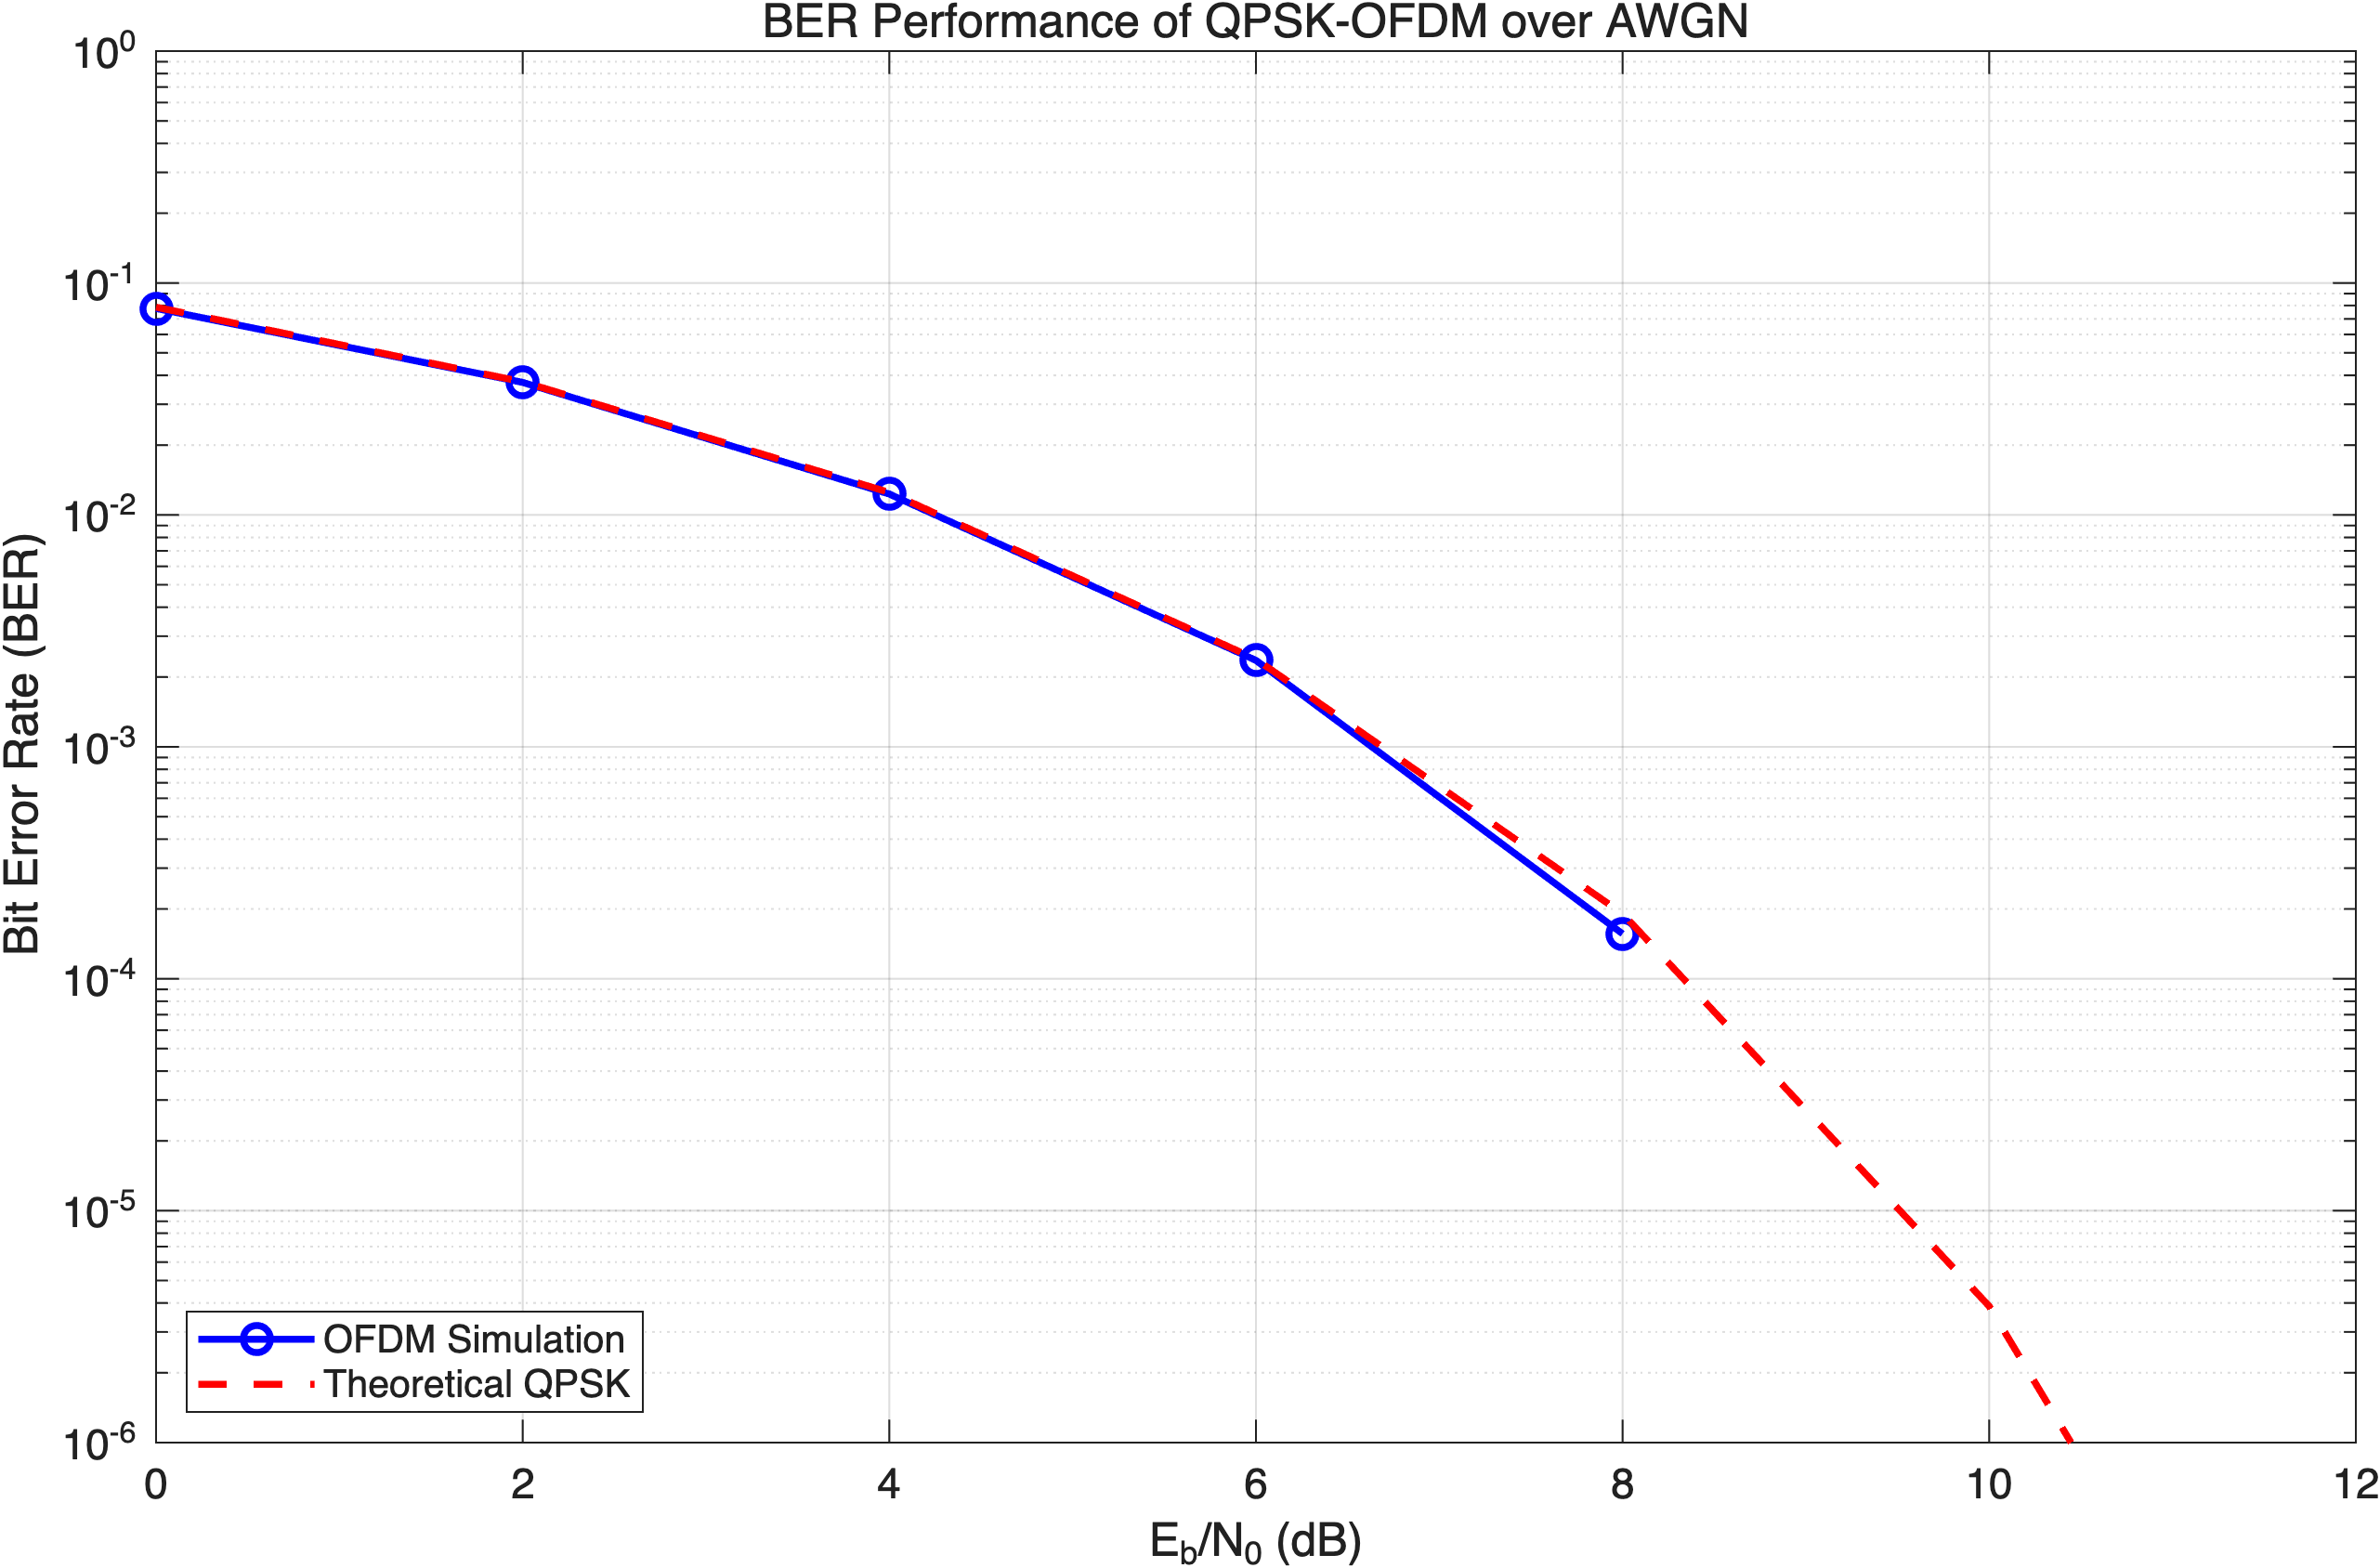
\includegraphics[width=.88\linewidth]{figures/ch4/exp01_ber_vs_ebn0.png}
\caption{EXP01: baseline QPSK--OFDM BER in AWGN. The logarithmic plot omits simulated zero-error observations and shows the low-$E_b/N_0$ range.}
\label{fig:ch4_baseline}
\end{figure}

The numerical agreement at low and moderate $E_b/N_0$ supports the consistency of modulation, IFFT/FFT processing, CP removal and the noise convention used in the baseline. No bit errors are observed from 10 through 20 dB. This does not establish zero theoretical BER: for example, the theoretical probability at 10 dB is $3.87\times10^{-6}$, corresponding to fewer than one expected error in 128,000 bits. The finite experiment therefore cannot resolve very small probabilities. The baseline horizontal axis is useful-data $E_b/N_0$, not the received active-frame SNR of EXP07.

\section[Controlled Timing Offsets]{Sensitivity to Controlled Timing Offsets}
\label{sec:ch4_offset}
EXP02 imposes known integer displacements of the FFT window rather than obtaining them from an estimator. This isolates the receiver's response to timing error. The noiseless frequency-domain experiment scans offsets from $-24$ to $+24$ samples. As shown in Figure~\ref{fig:ch4_offset_mse}, nonzero offsets within the single-path CP-safe region produce frequency-domain MSE of 2 (relative to unit-energy transmitted subcarrier symbols), despite preserving subcarrier magnitudes. Indeed, for a nonzero integer shift $e$ with $|e|<N$, the geometric-sum identity gives
\begin{equation}
\frac{1}{N}\sum_{k=0}^{N-1}\left|\exp(j2\pi ke/N)-1\right|^2=2.
\end{equation}
This is a symbol-domain error measure, not the timing-estimation MSE in samples squared. The distinction is important throughout the chapter.

\begin{figure}[!htbp]
\centering
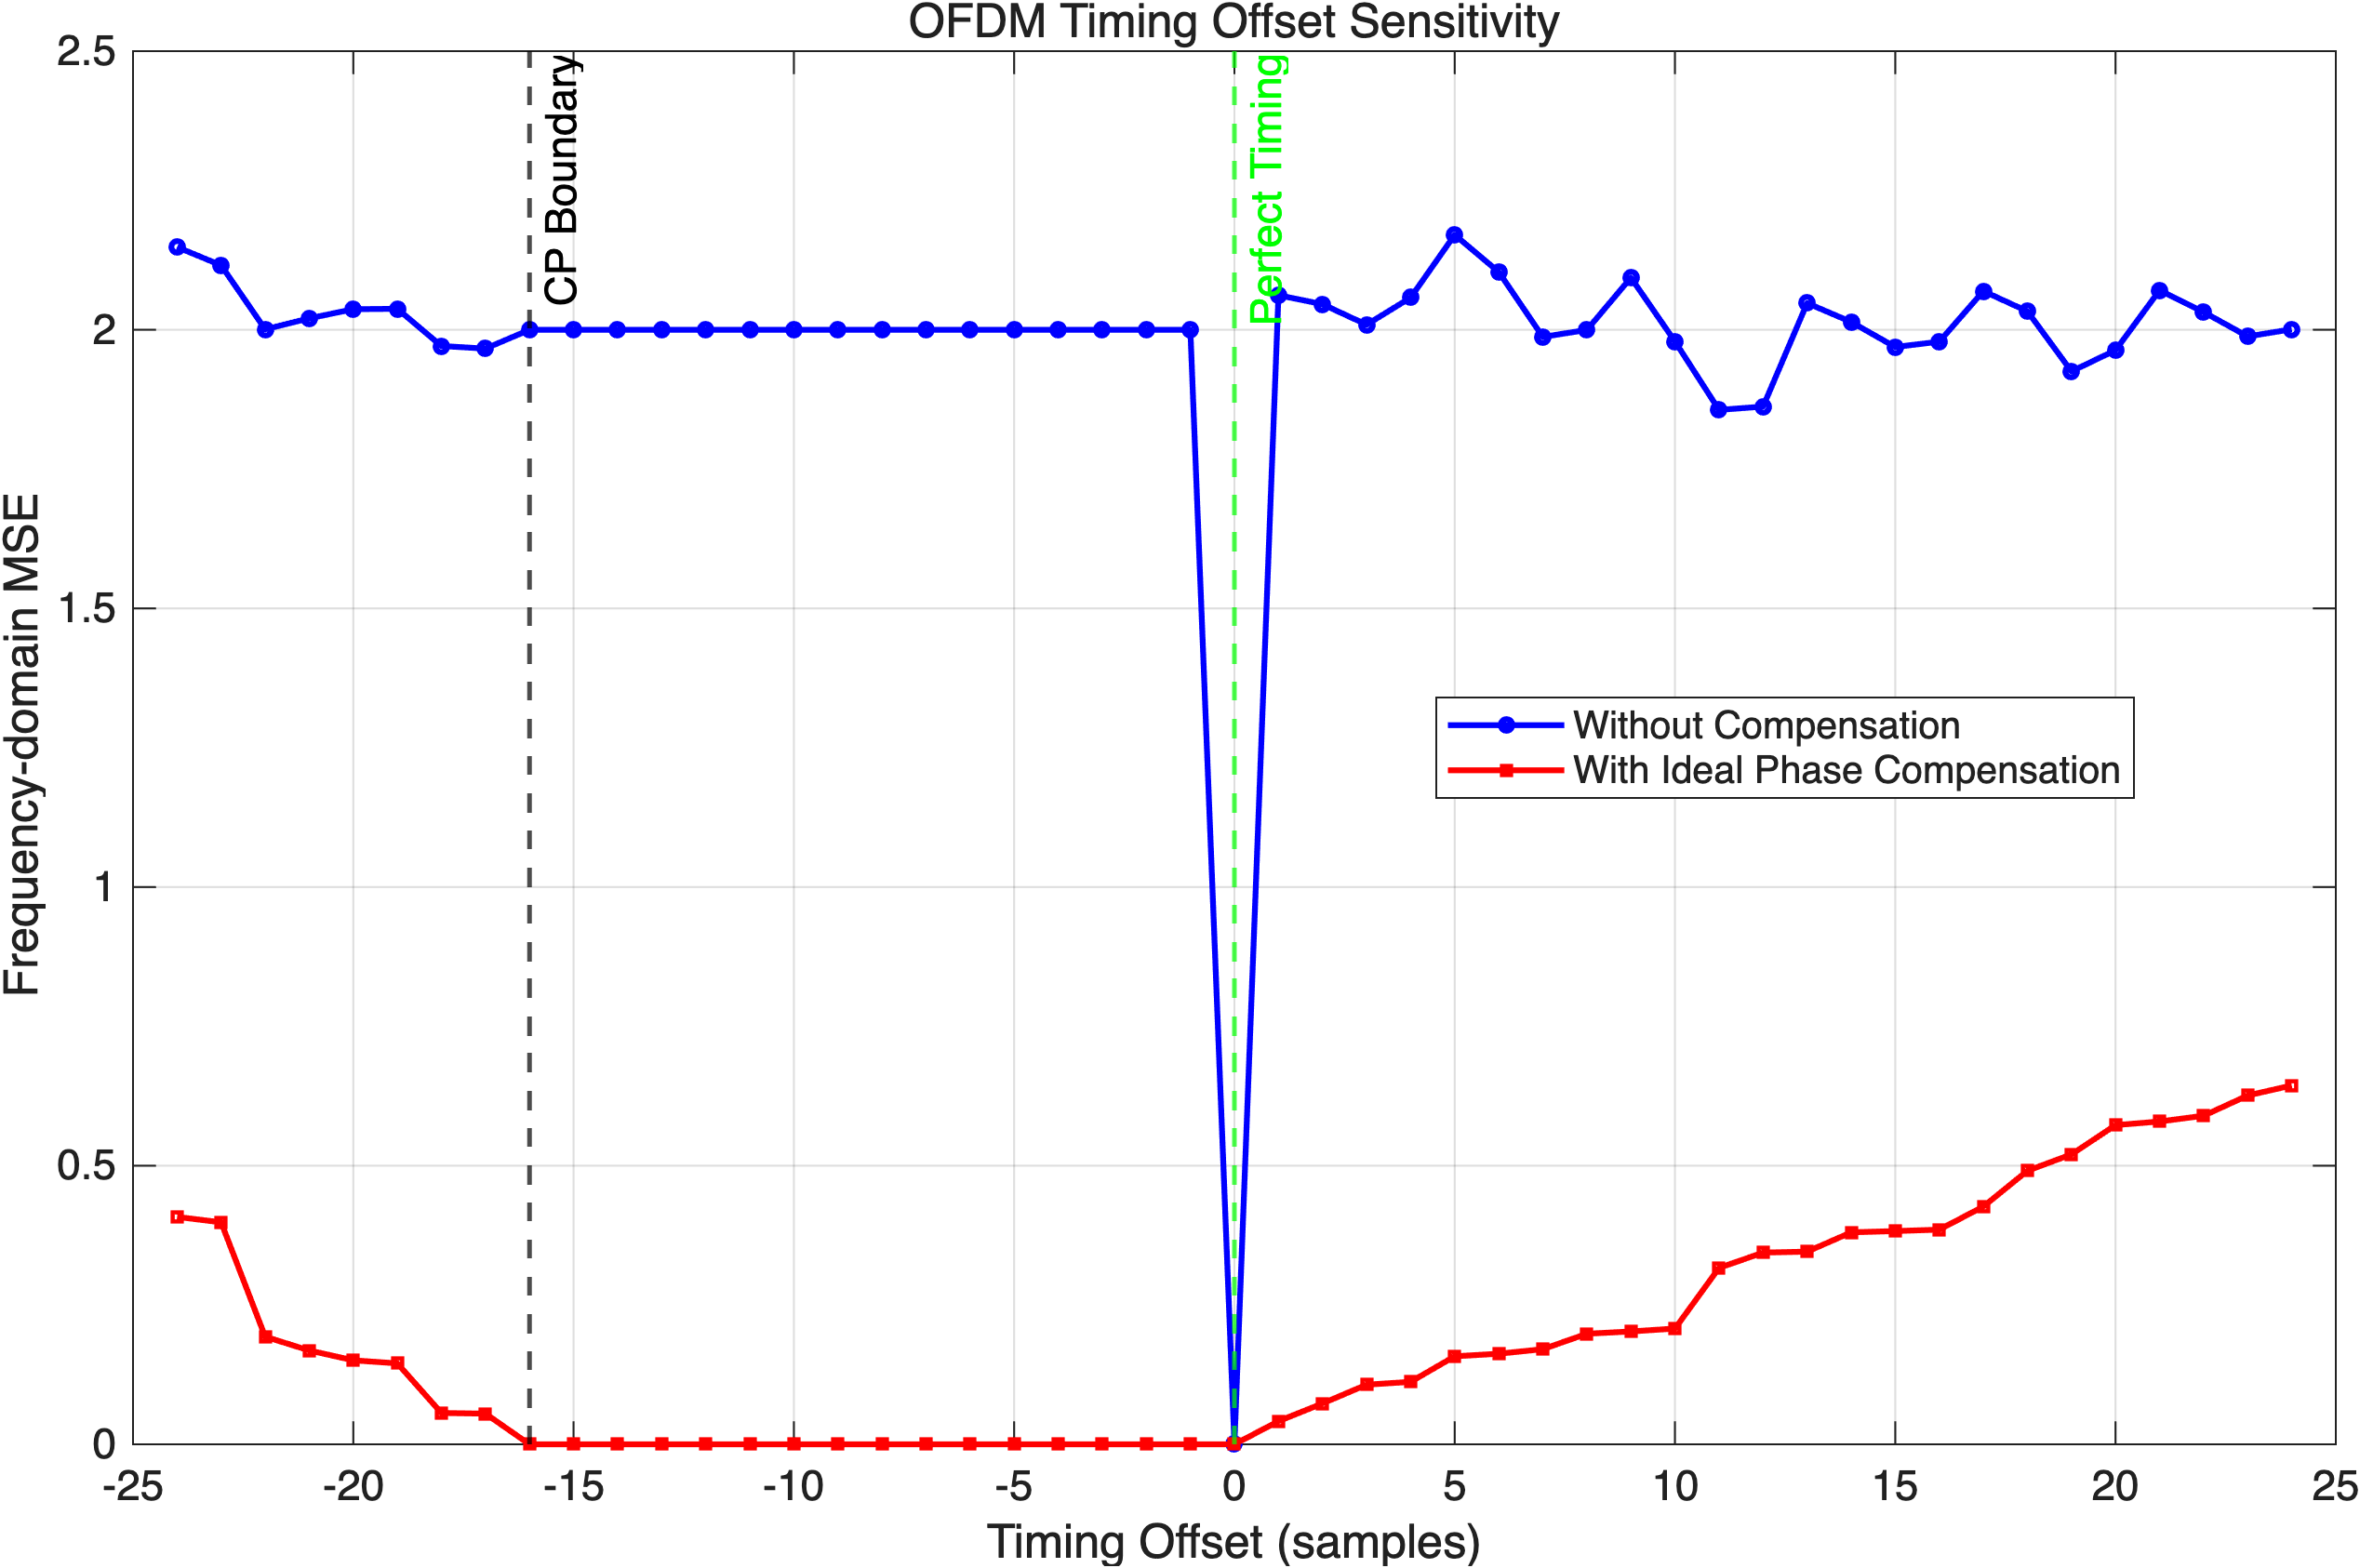
\includegraphics[width=.88\linewidth]{figures/ch4/exp02_timing_offset_sensitivity.png}
\caption{EXP02: noiseless frequency-domain MSE with and without phase compensation.}
\label{fig:ch4_offset_mse}
\end{figure}

At $e=-5$, the uncompensated frequency-domain MSE is 2, while phase compensation reduces it to approximately $1.78\times10^{-30}$. At $e=+5$, the compensated MSE remains approximately 0.1579. The latter window includes samples beyond the current useful symbol; thus the ideal circular-shift relation cannot account for the entire observation. The boundary at $-16$ is likewise visible in the compensated MSE curve.

The noiseless BER scan in Figure~\ref{fig:ch4_offset_ber} confirms the detection consequences. At $e=-5$, uncompensated BER is 0.498680, whereas compensation yields zero observed errors; at $e=+5$, the compensated BER is 0.008422. At $e=+24$ it rises to 0.215477. Some offsets outside the safe region still yield zero observed errors after compensation (for example, $e=-18$), but the frequency-domain distortion is nonzero. The CP-safe criterion is a sufficient structural condition, not a necessary condition for every finite set of QPSK decisions to be correct.

\begin{figure}[!htbp]
\centering
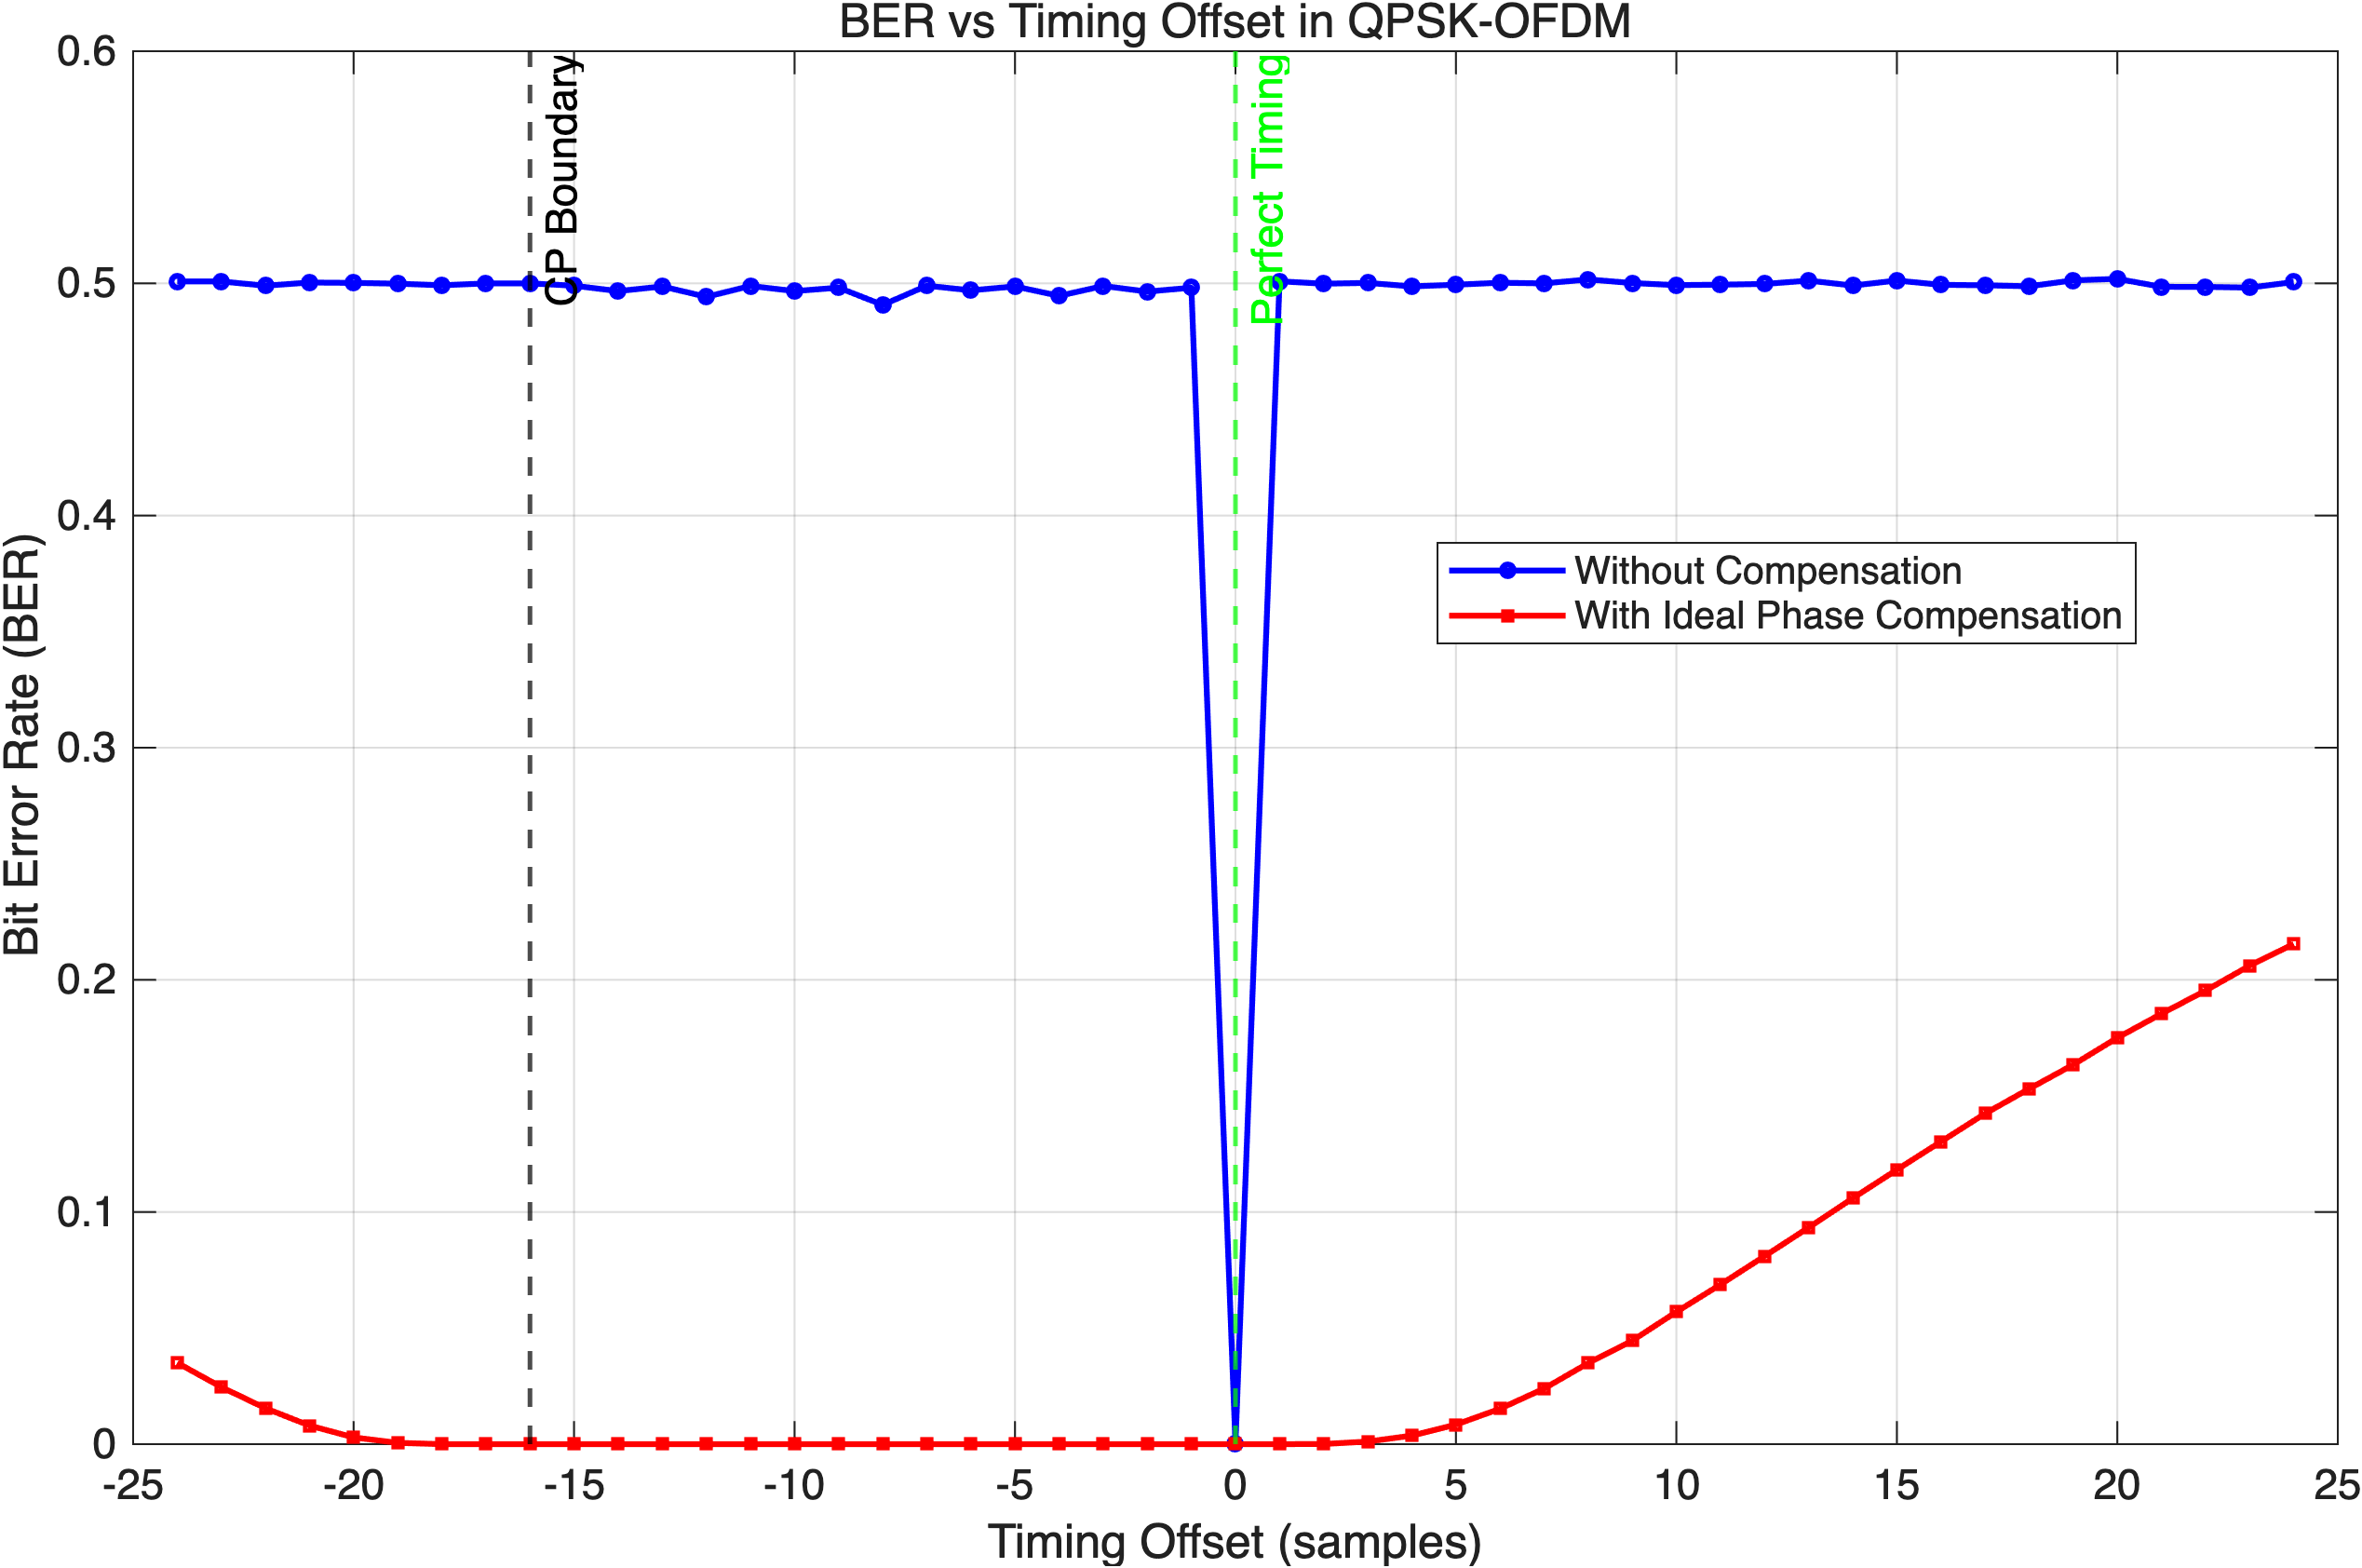
\includegraphics[width=.88\linewidth]{figures/ch4/exp02_ber_vs_timing_offset.png}
\caption{EXP02: noiseless BER for imposed FFT-window displacements, using 128,000 data bits.}
\label{fig:ch4_offset_ber}
\end{figure}

A separate AWGN experiment compares the perfect window, a five-sample early window with and without phase compensation, and a five-sample late window with compensation. Figure~\ref{fig:ch4_offset_snr} shows that the compensated early window closely tracks perfect timing. At $E_b/N_0=8$ dB, both record 21 bit errors, while the late compensated window records 3,292. At 12 dB, the perfect and compensated early cases record no errors, but the late compensated case records 1,898 (BER 0.014828). Uncompensated early-window BER stays close to 0.5. These results support the phase-rotation explanation of Chapter 2 and motivate a separate evaluation of CP-safe and exact timing probabilities.

\begin{figure}[!htbp]
\centering
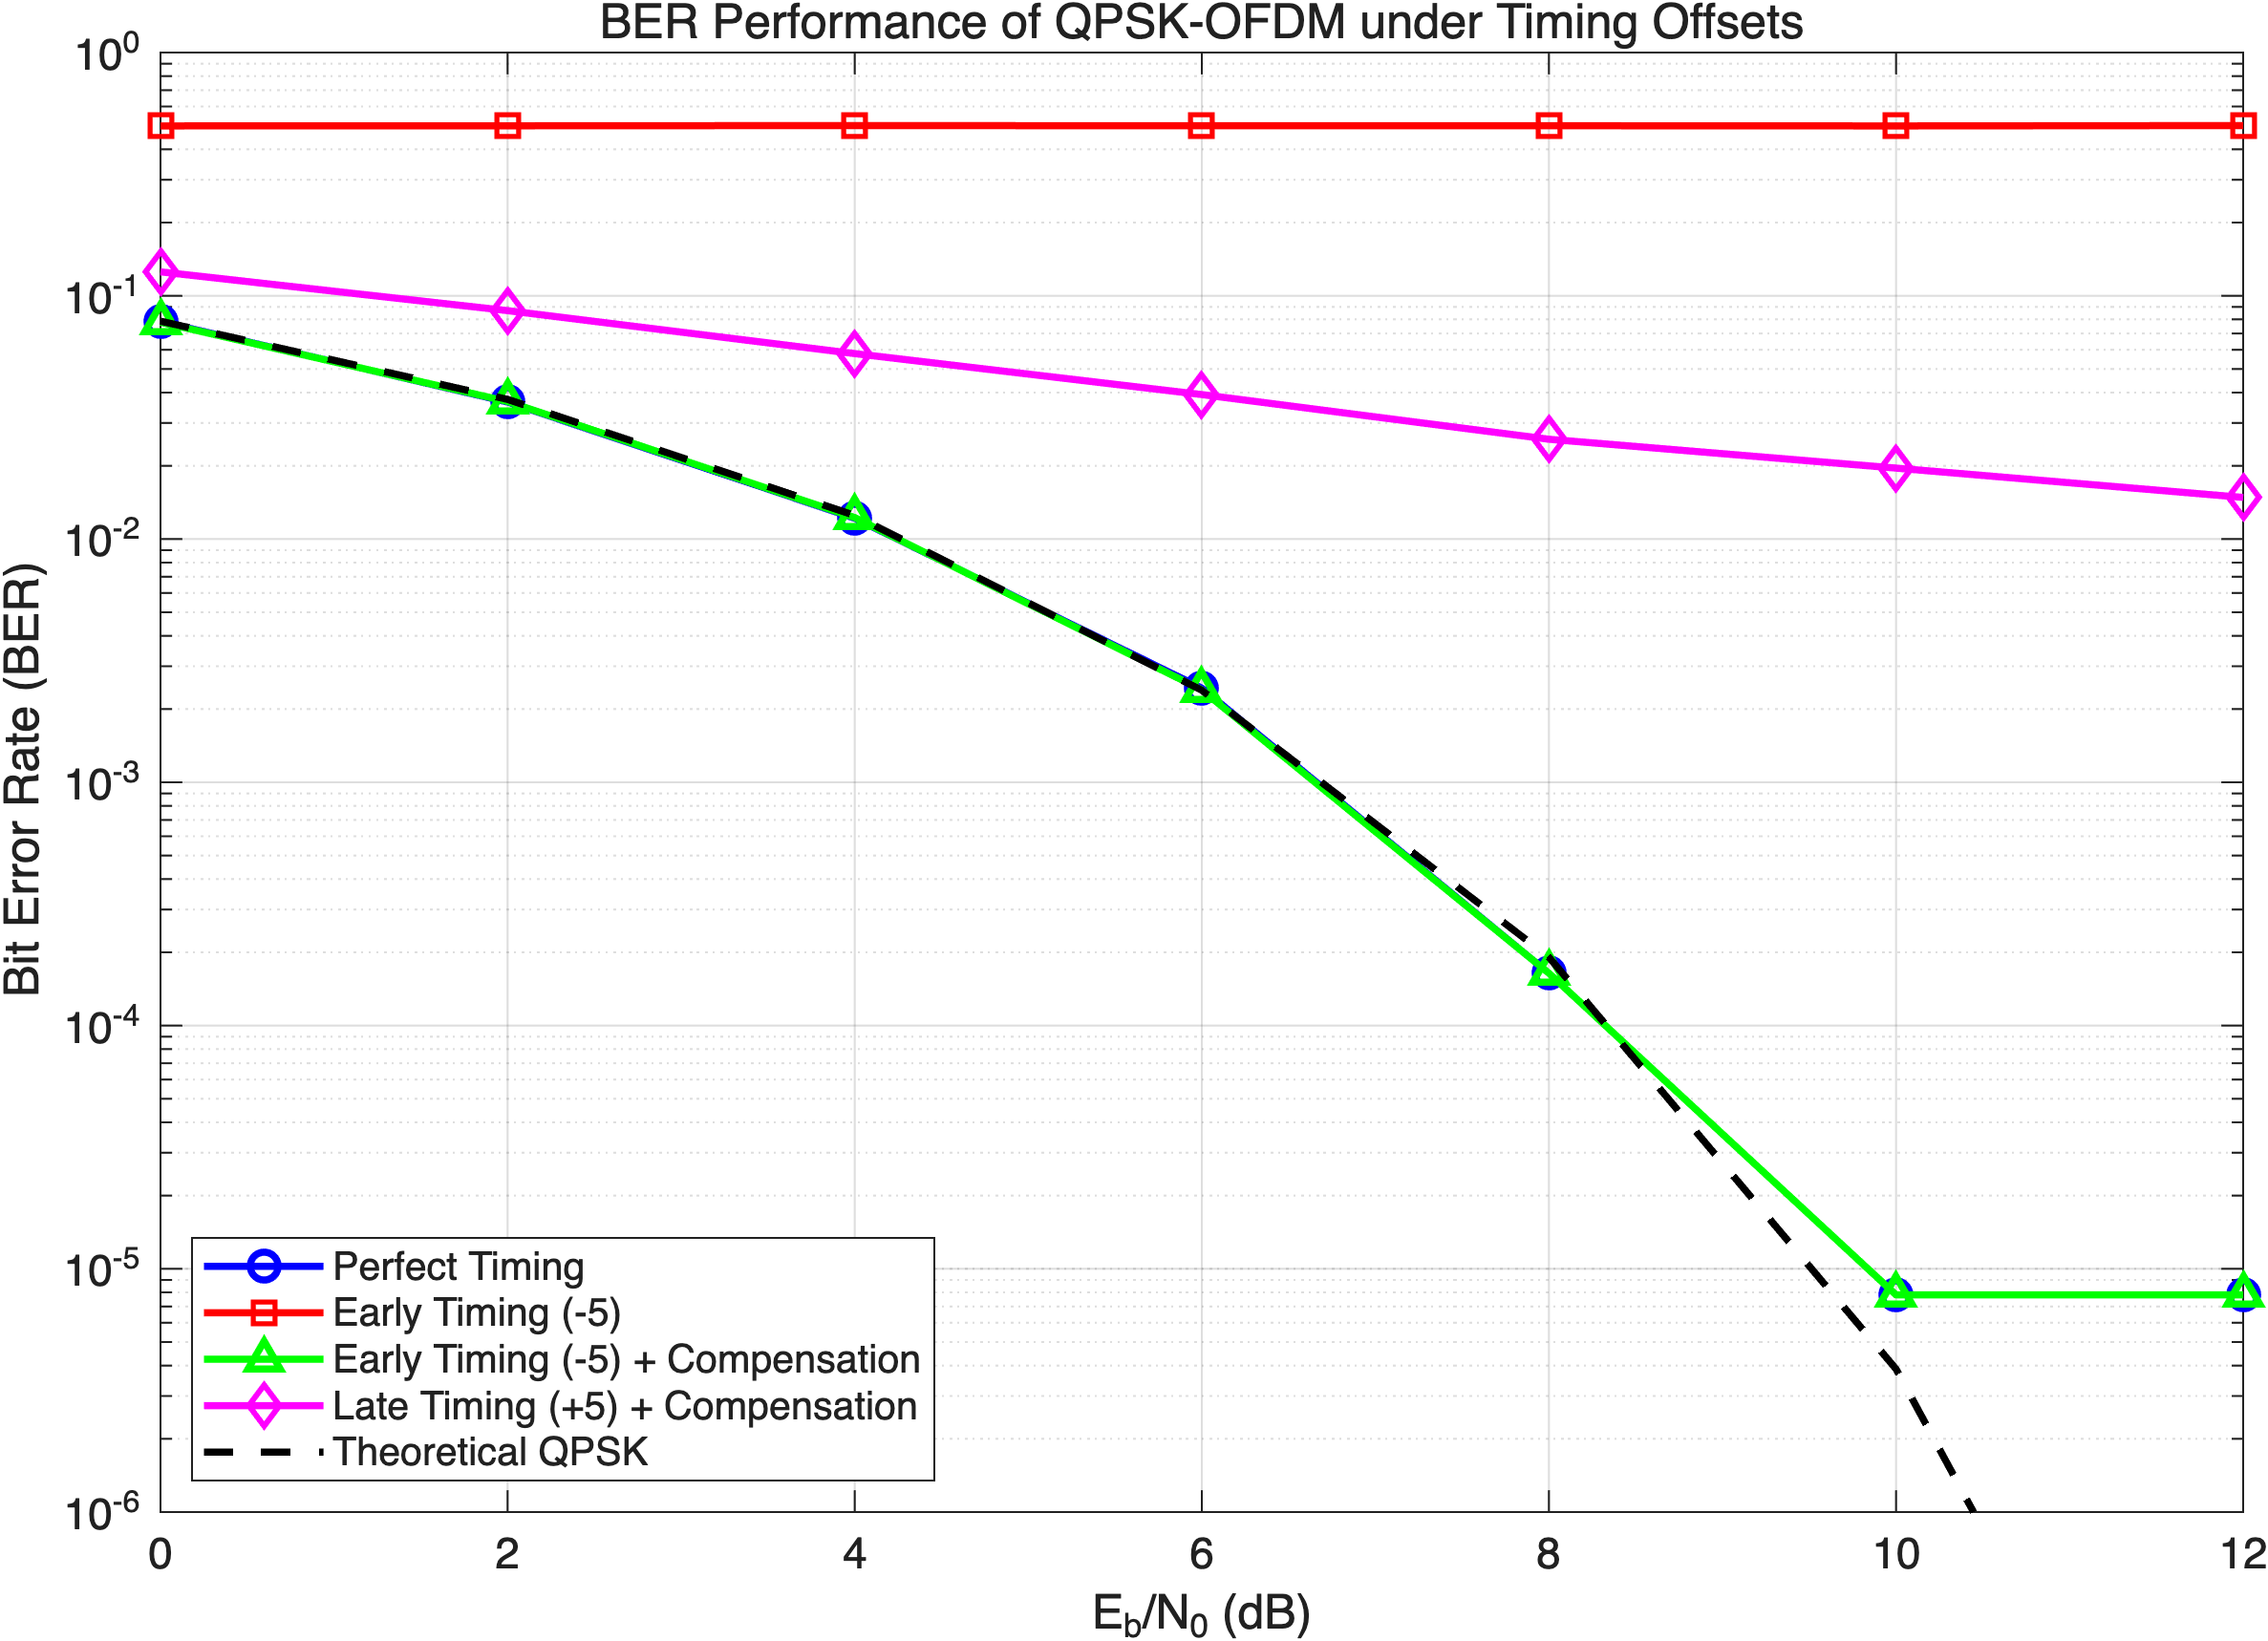
\includegraphics[width=.88\linewidth]{figures/ch4/exp02_ber_vs_ebn0.png}
\caption{EXP02: BER under AWGN with imposed timing offsets. Observed zero BER values are displayed at $1/128000$ for logarithmic plotting only.}
\label{fig:ch4_offset_snr}
\end{figure}

\section[Individual Estimator Checks]{Individual Estimator Validation}
\label{sec:ch4_individual}
EXP03--06 establish that the implemented timing metrics and decision rules operate before the formal comparison. These experiments are not used to rank the four methods because the earlier search settings and random scenarios are not identical.

In the noiseless S\&C verification (EXP03), the arrival delay is 50 samples and the true useful start is 67 in MATLAB indexing. The metric remains at one from candidate 51 to 67 inclusive, a plateau covering the CP and the true start. Figure~\ref{fig:ch4_plateau} shows this ambiguity. The individual AWGN Monte Carlo experiment records an exact probability of 0.0010 but a CP-safe probability of 0.9999 at 20 dB. These values already indicate that low noise does not remove the systematic displacement caused by a plateau-midpoint decision.

\begin{figure}[!htbp]
\centering
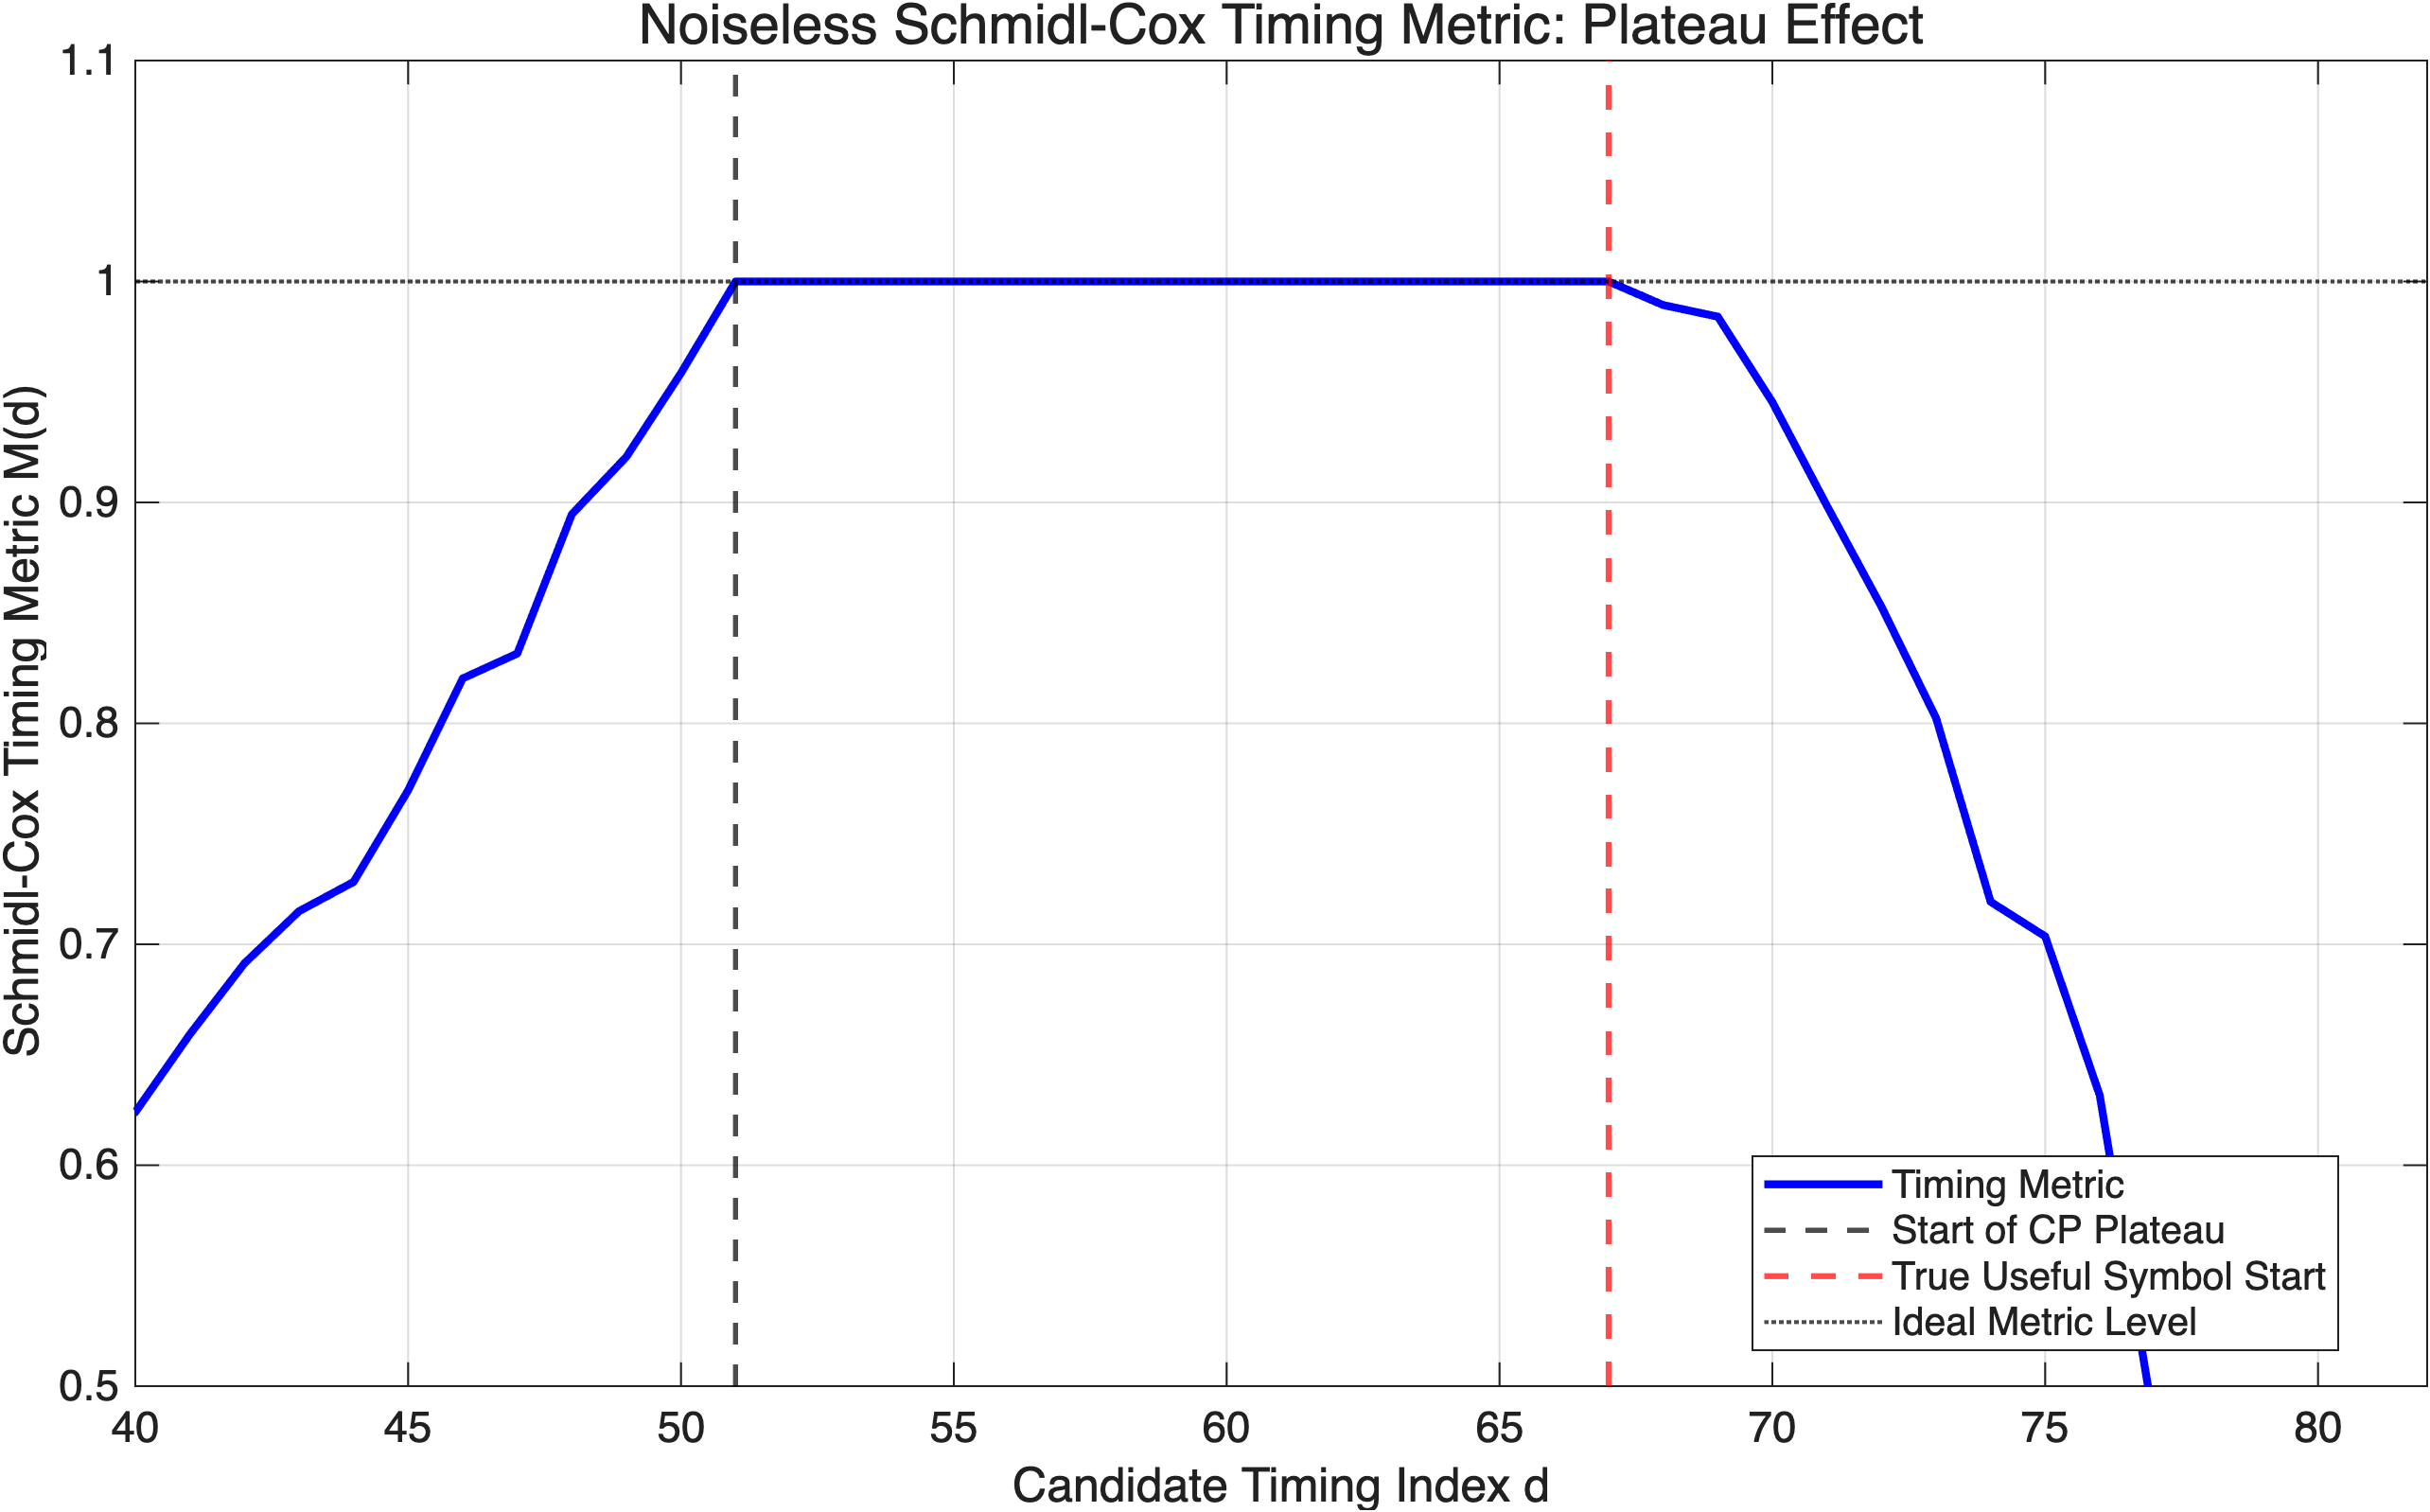
\includegraphics[width=.88\linewidth]{figures/ch4/sc_noiseless_timing_metric_zoom.png}
\caption{EXP03: noiseless S\&C plateau, with the CP start at 51 and useful-symbol start at 67.}
\label{fig:ch4_plateau}
\end{figure}

The final Park-type experiment (EXP04) records exact probabilities of 0.9184 in AWGN and 0.5442 in the fixed multipath channel at 0 dB. By 10 dB these become 1.0000 and 0.9895. Earlier Park structure and normalization diagnostics are not substituted for the final supervisor-confirmed version. In EXP05, the Minn-type estimator gives exact probabilities of 0.6153 and 0.4564 in AWGN and multipath at 0 dB, rising to 0.9991 and 0.9957 at 10 dB. In EXP06, CAZAC records exact probability 1.0000 throughout the AWGN grid and 0.9996 at 0 dB in the fixed multipath channel. These checks motivate the unified comparison; their numerical values should not be pooled with EXP07 results.

\section[Unified Timing Metrics]{Timing Metric Examples in EXP07}
\label{sec:ch4_metrics}
The representative metric experiment uses a fixed arrival delay $D=50$ and maps each algorithm's candidate indices to the common useful-start coordinate. The true useful training start is 67. The horizontal axes in Figures~\ref{fig:ch4_metric_ideal}--\ref{fig:ch4_metric_mp} show candidate error relative to this start. Each curve is normalized for display; these plotted heights must not be interpreted as identically calibrated decision metrics. The actual estimates are obtained from the algorithms and eligibility conditions specified in Chapter 3.

\begin{figure}[!htbp]
\centering
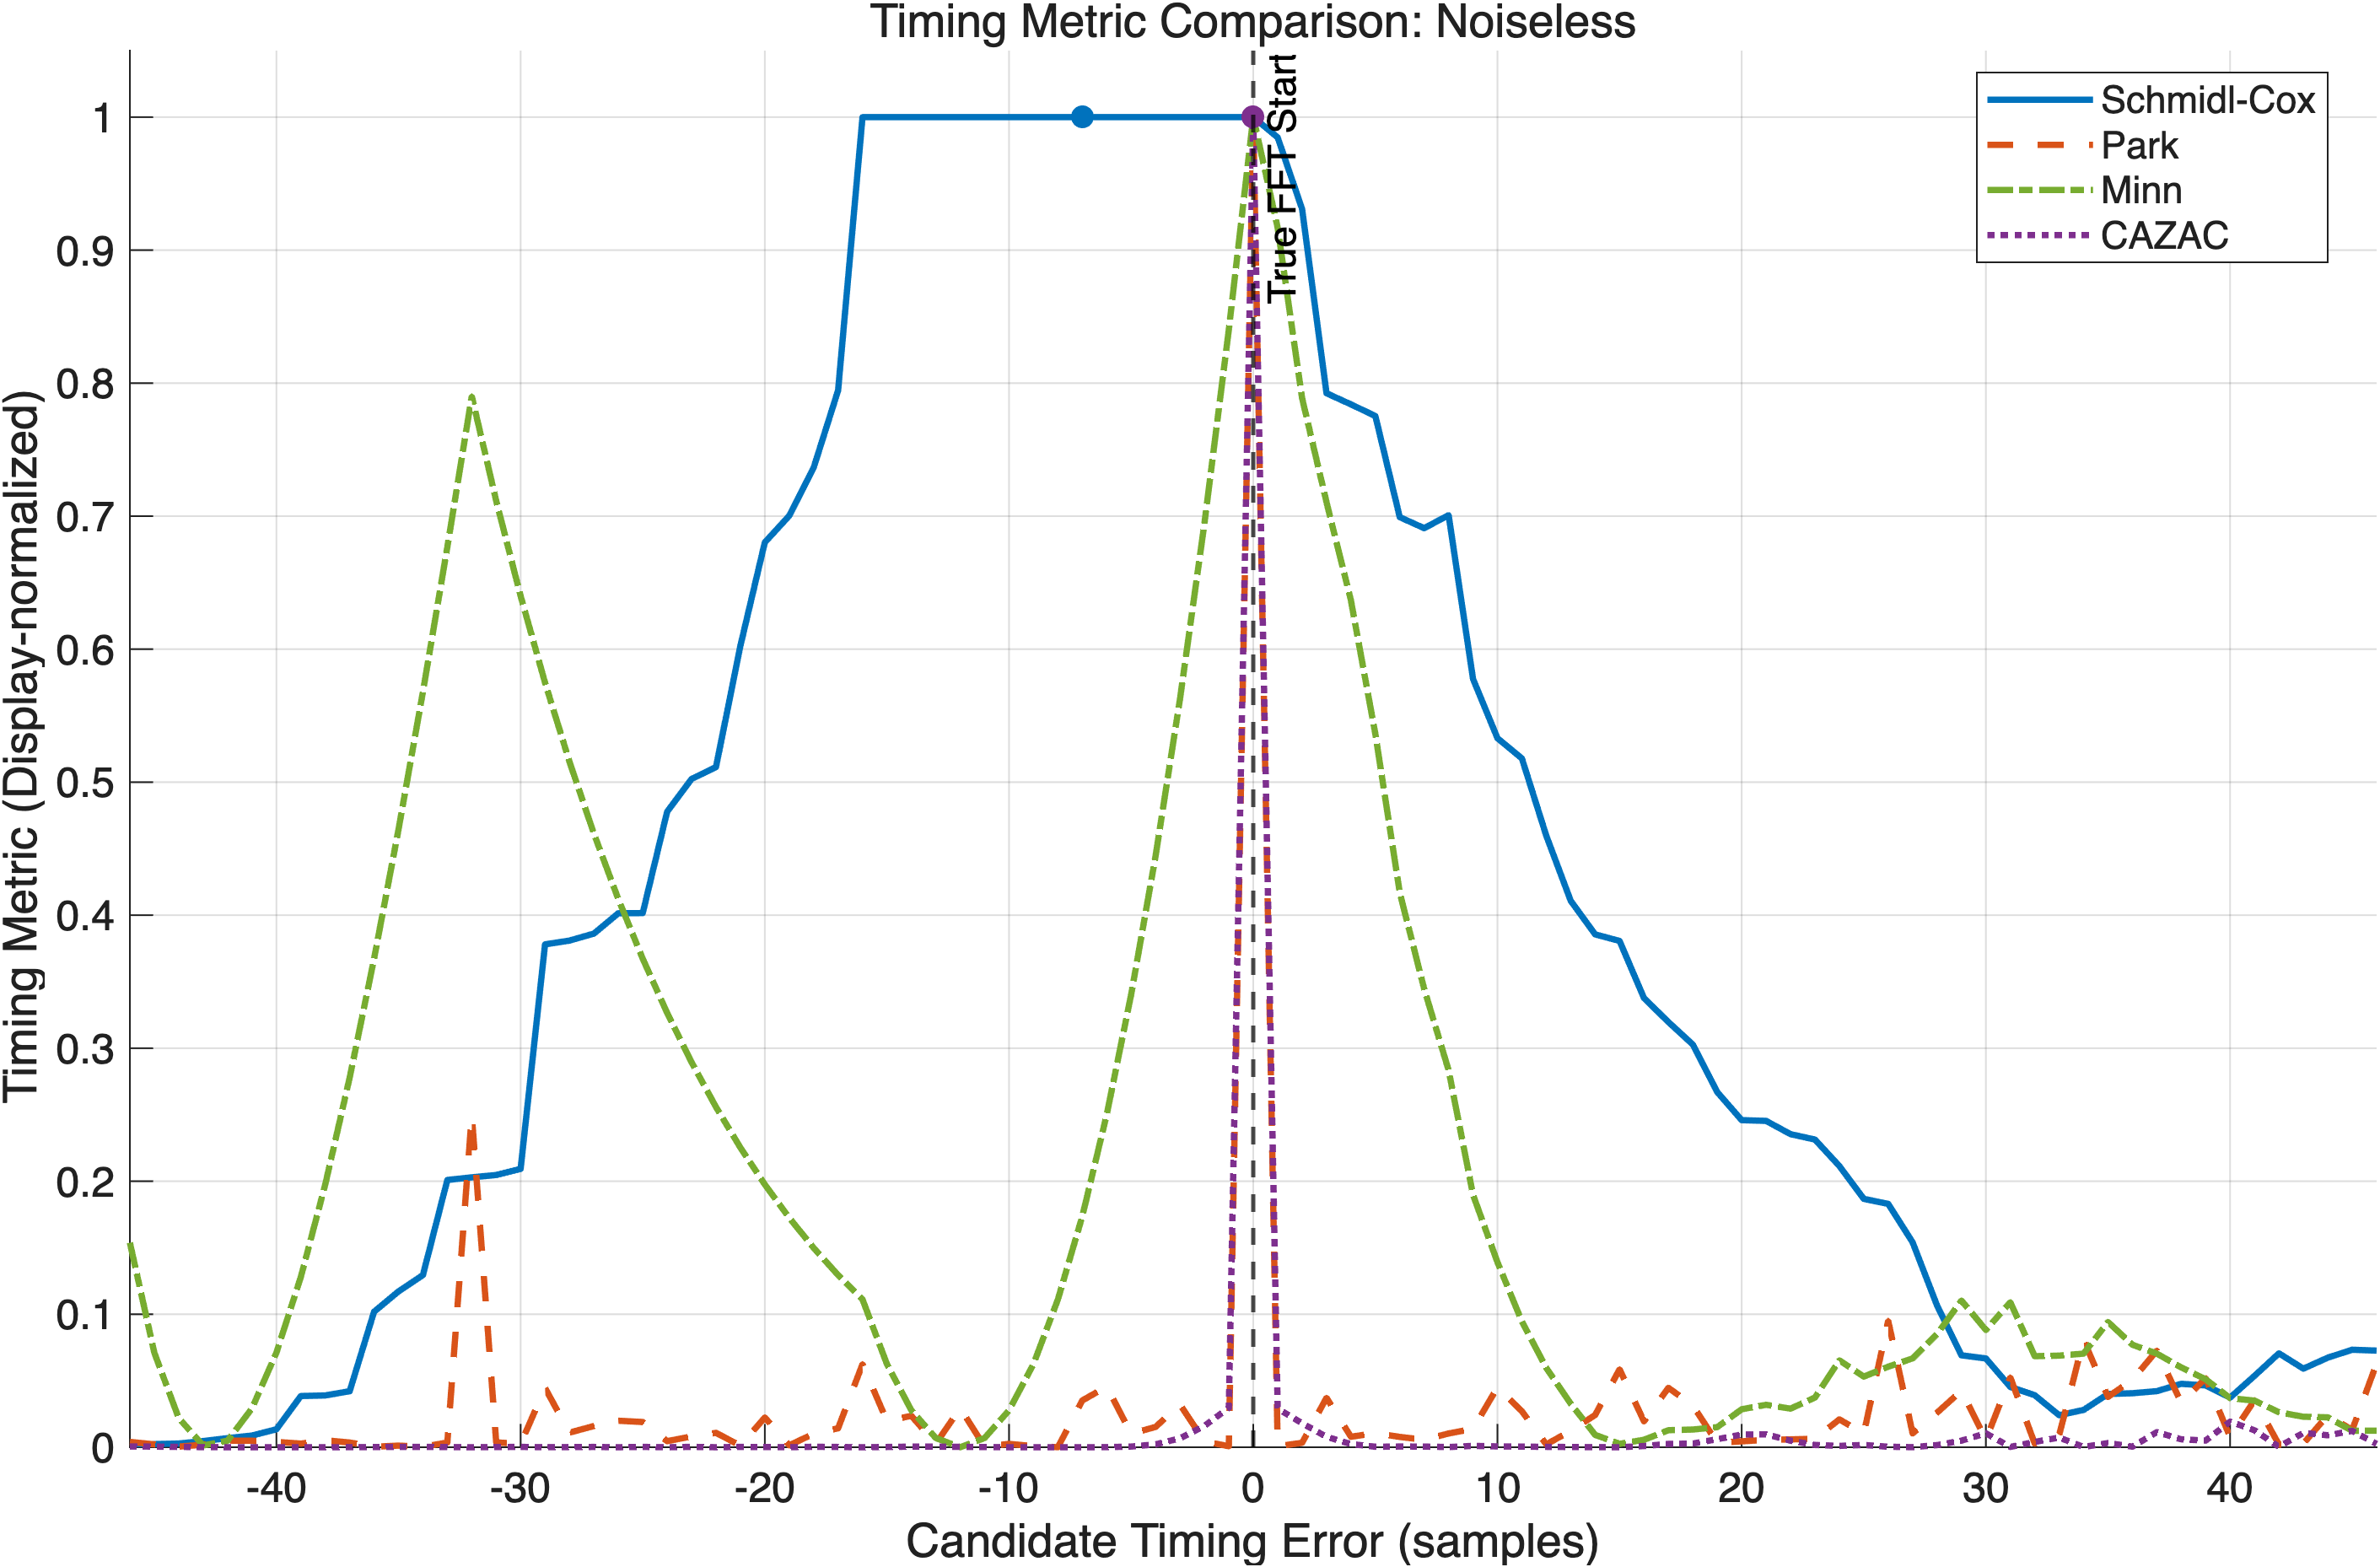
\includegraphics[width=.88\linewidth]{figures/ch4/exp07_metric_noiseless.png}
\caption{EXP07: display-normalized timing metrics in the noiseless single-path case.}
\label{fig:ch4_metric_ideal}
\end{figure}

\begin{figure}[!htbp]
\centering
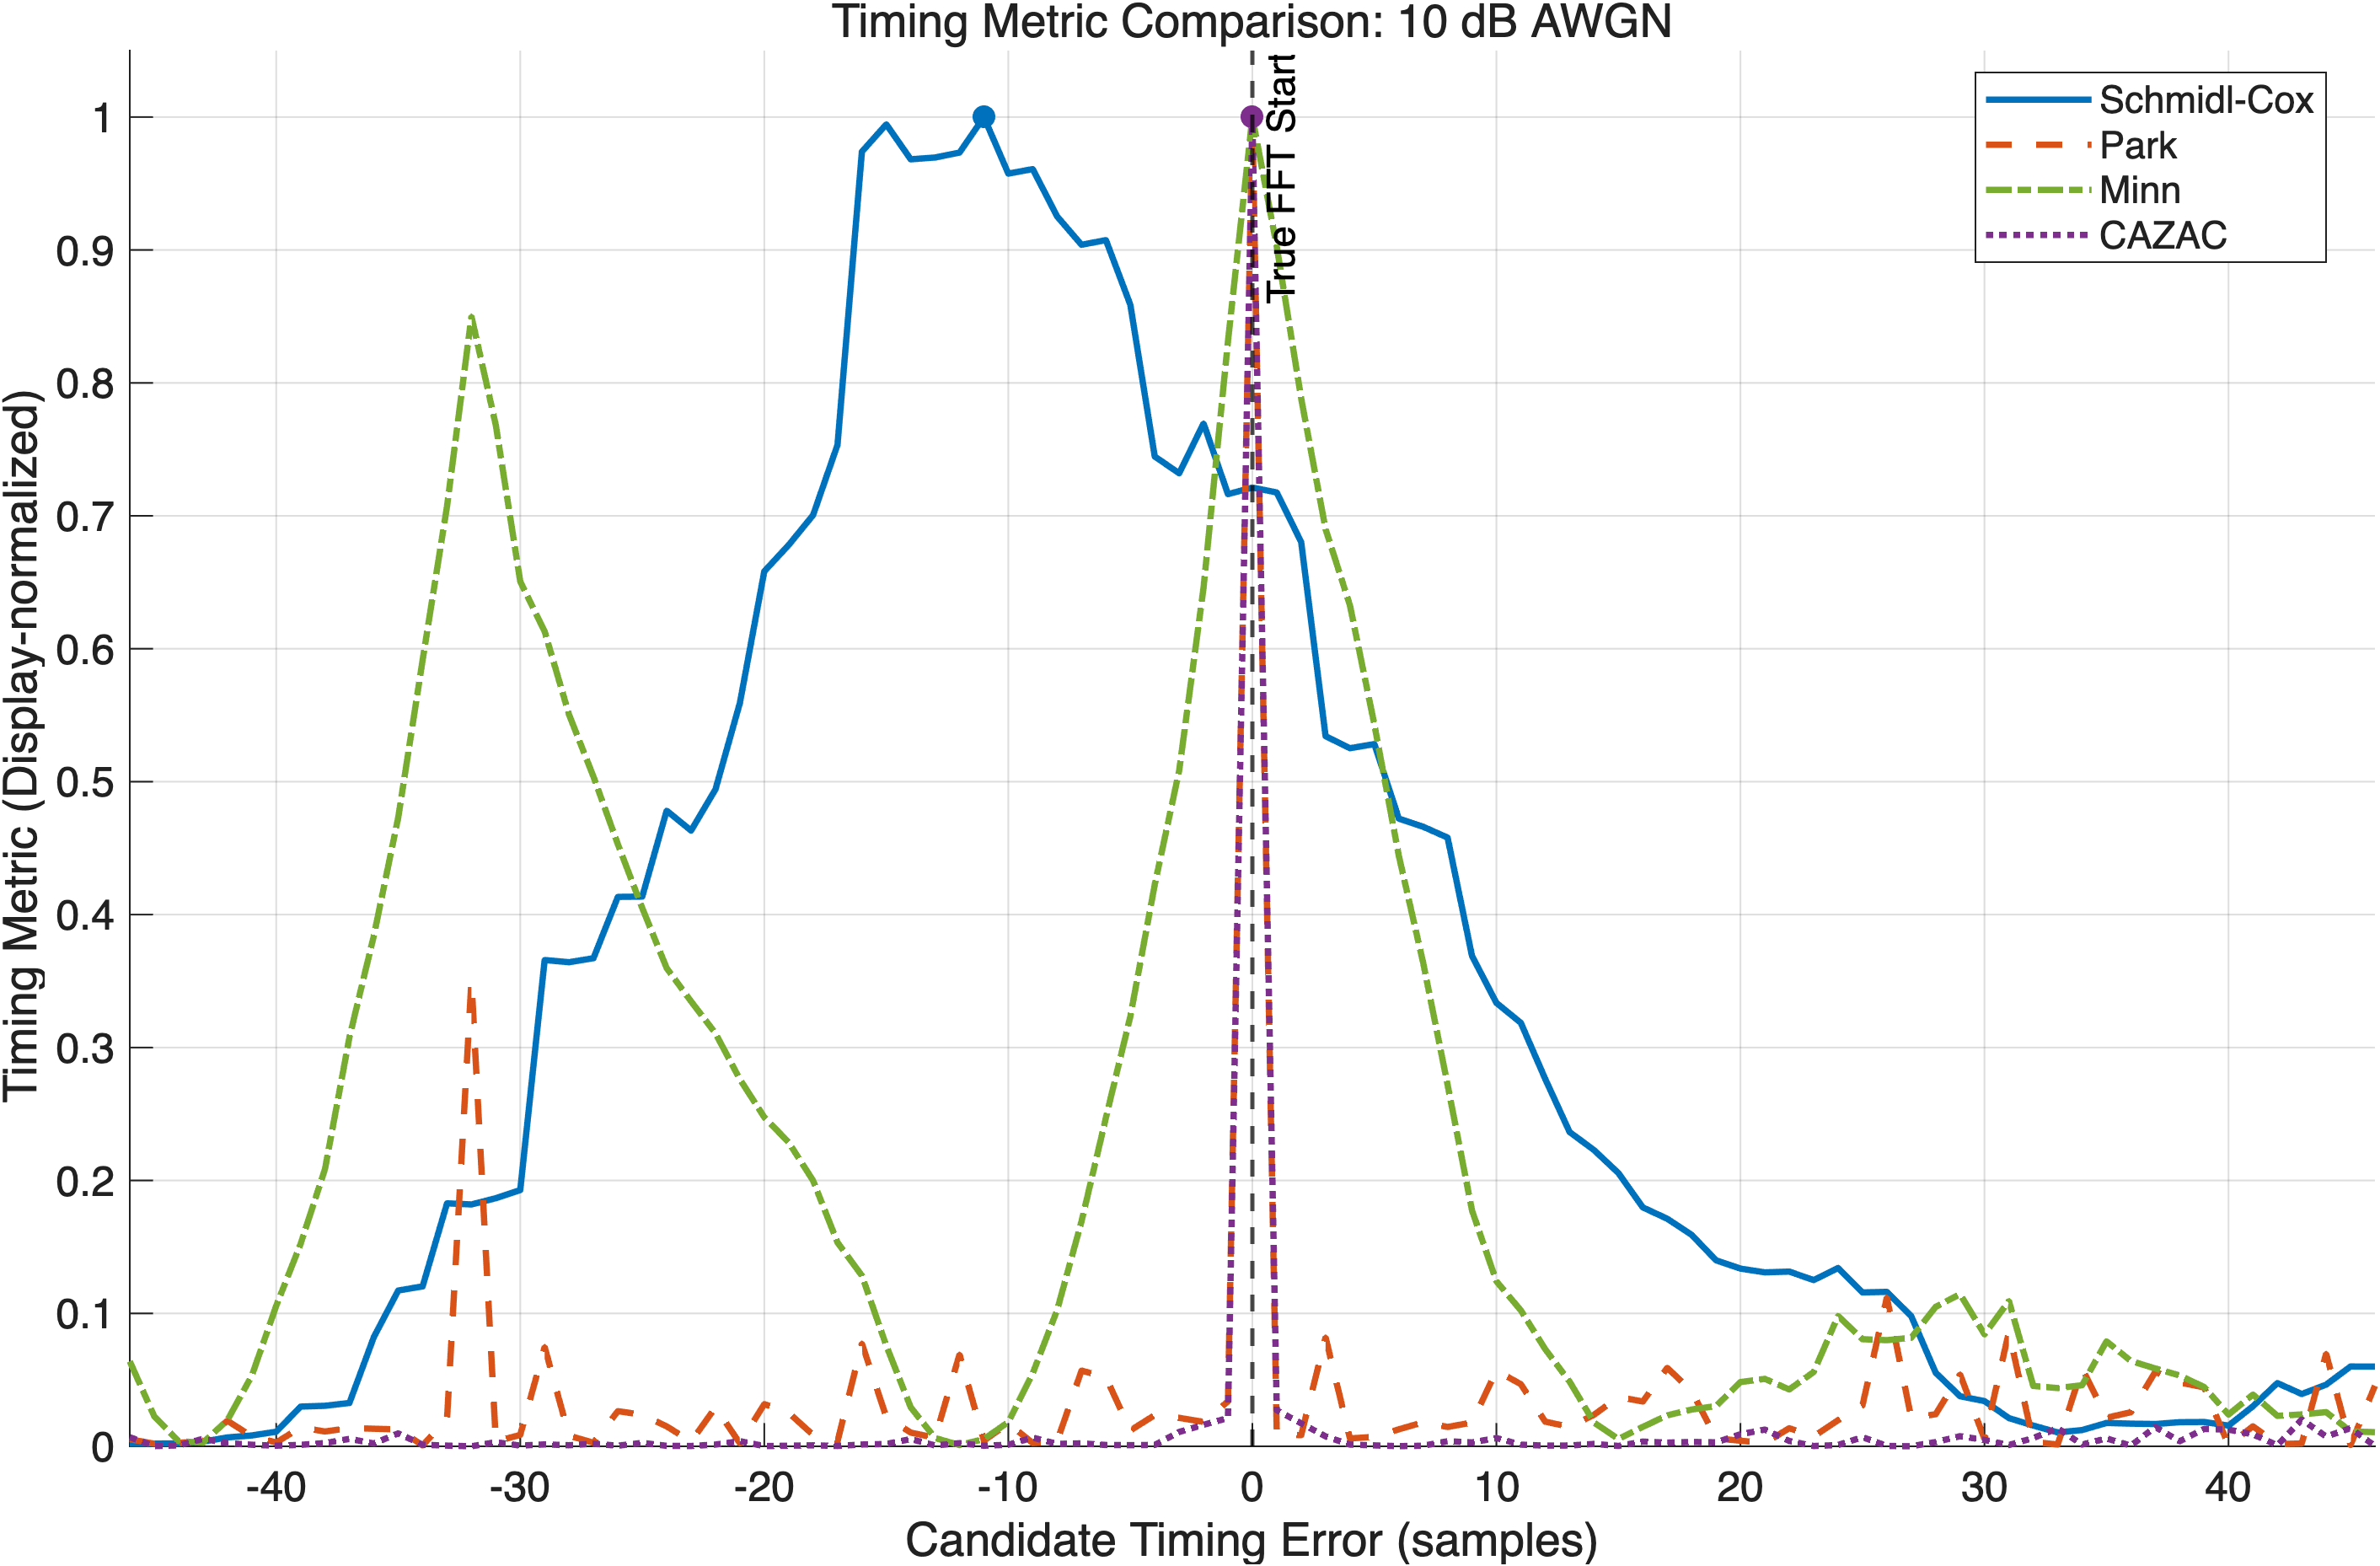
\includegraphics[width=.88\linewidth]{figures/ch4/exp07_metric_awgn_10dB.png}
\caption{EXP07: representative display-normalized timing metrics at 10 dB AWGN.}
\label{fig:ch4_metric_awgn}
\end{figure}

\begin{figure}[!htbp]
\centering
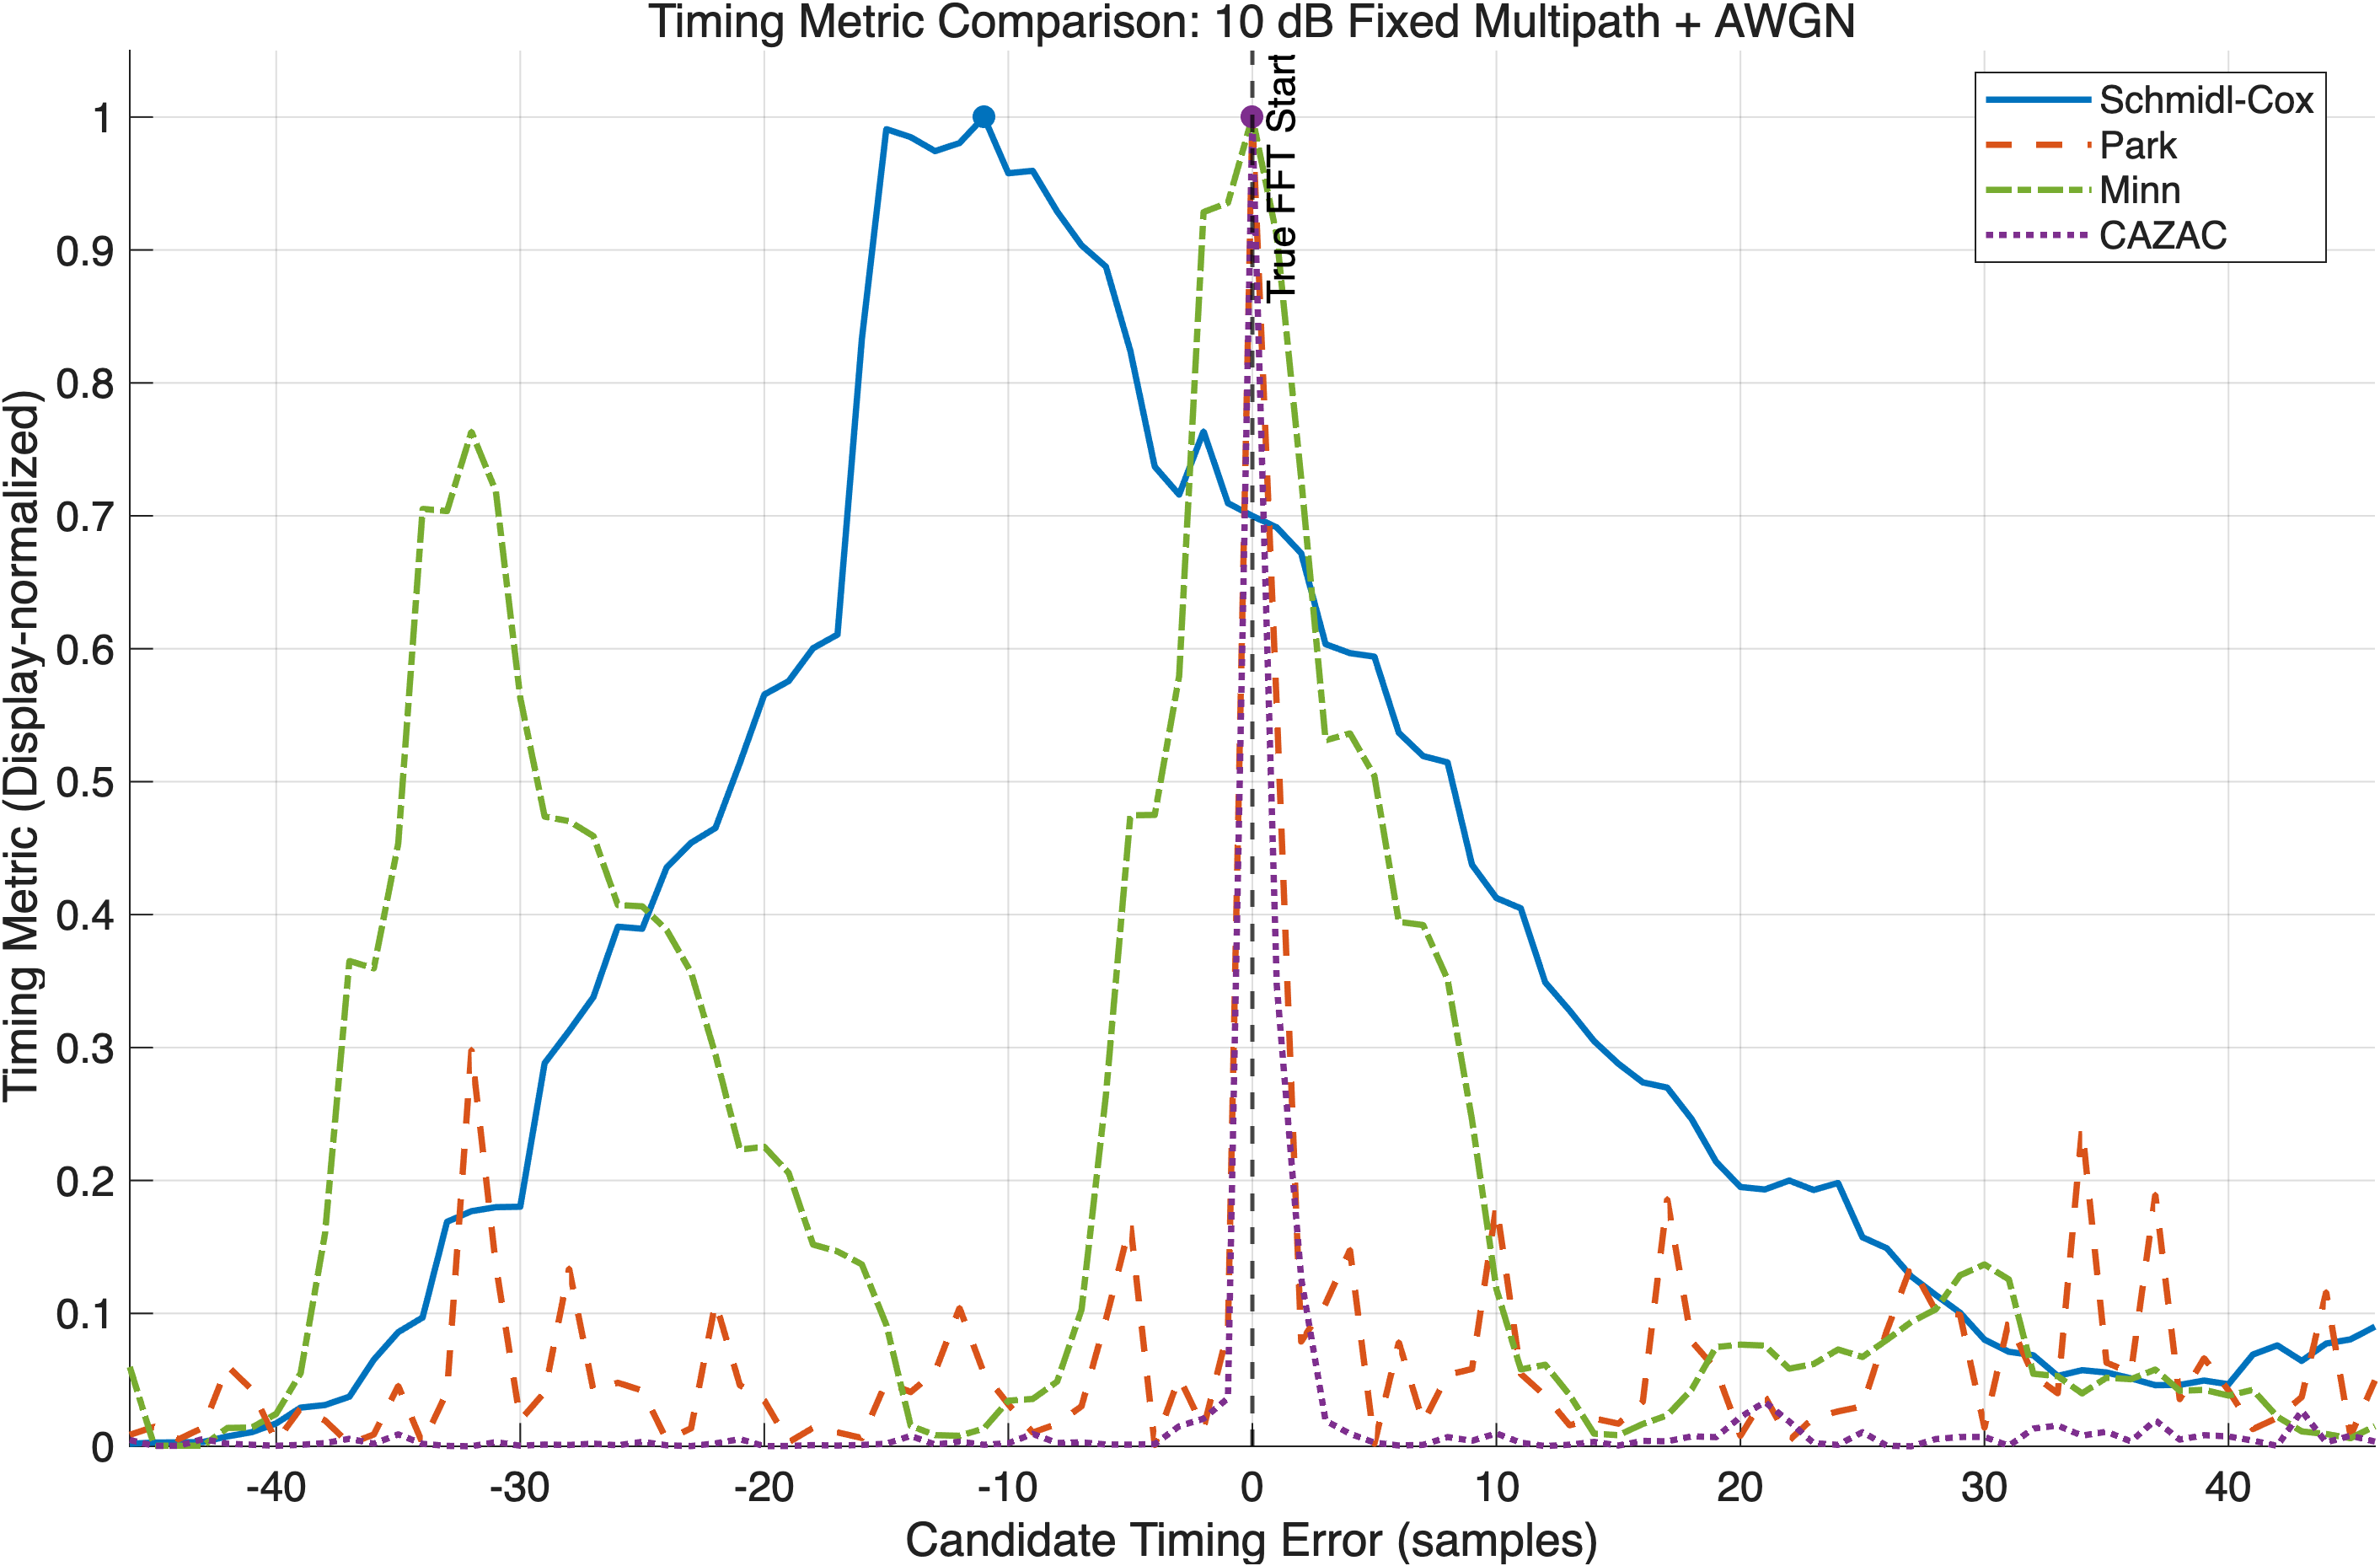
\includegraphics[width=.88\linewidth]{figures/ch4/exp07_metric_multipath_10dB.png}
\caption{EXP07: representative display-normalized timing metrics at 10 dB in fixed multipath.}
\label{fig:ch4_metric_mp}
\end{figure}

\begin{table}[htbp]
\centering
\caption{Timing errors in the three representative EXP07 frames (samples).}
\label{tab:ch4_examples}
\begin{tabular}{lrrrr}
\hline
Scenario & S\&C & Park & Minn & CAZAC\\
\hline
Noiseless & $-7$ & 0 & 0 & 0\\
AWGN, 10 dB & $-11$ & 0 & 0 & 0\\
Multipath, 10 dB & $-11$ & 0 & 0 & 0\\
\hline
\end{tabular}
\end{table}
The S\&C curve displays a broad plateau or rounded high-metric region; the three other methods provide a more localized maximum near the reference in these particular observations. Minn also exhibits a competing peak approximately 32 samples before the useful start, consistent with its signed-block structure. The Park metric is affected by local symmetry and multipath, while CAZAC uses the complete known template. Table~\ref{tab:ch4_examples} reports the actual decisions. The three peak-based methods return the true start in all three displayed frames; S\&C selects an early position. A single representative observation cannot establish the probability of choosing a competing peak, so statistical comparison is required.

\section[Unified Monte Carlo Results]{Unified Monte Carlo Timing Results}
\label{sec:ch4_comparison}
EXP07 contains 10,000 estimates for every algorithm, SNR and channel combination, giving 880,000 attempted timing estimates. All are valid, and all 88 condition-level summaries have zero observed no-estimate events. This is not a claim that every estimate is correct or that a noise-only frame would be rejected. Tables~\ref{tab:ch4_awgn} and~\ref{tab:ch4_mp} report representative SNR levels; Figures~\ref{fig:ch4_mse}--\ref{fig:ch4_cpsafe} show the full grid. Since no estimate is invalid, the conditional MSE equals the empirical MSE over all 10,000 attempts in each condition.

\begin{table}[htbp]
\centering
\caption{EXP07 timing performance in AWGN at selected SNRs. MSE is in samples squared.}
\label{tab:ch4_awgn}
\small
\begin{tabular}{rlrrr}
\hline
SNR (dB) & Method & Exact & CP-safe & MSE\\
\hline
0 & S\&C & 0.0576 & 0.6773 & 135.9962 \\
 & Park & 0.8981 & 0.9132 & 100.1021 \\
 & Minn & 0.6438 & 0.7384 & 116.1906 \\
 & CAZAC & 1.0000 & 1.0000 & 0.0000 \\
\hline
10 & S\&C & 0.0385 & 0.9501 & 81.6839 \\
 & Park & 1.0000 & 1.0000 & 0.0000 \\
 & Minn & 0.9989 & 0.9989 & 0.9218 \\
 & CAZAC & 1.0000 & 1.0000 & 0.0000 \\
\hline
20 & S\&C & 0.0006 & 0.9978 & 59.4513 \\
 & Park & 1.0000 & 1.0000 & 0.0000 \\
 & Minn & 1.0000 & 1.0000 & 0.0000 \\
 & CAZAC & 1.0000 & 1.0000 & 0.0000 \\
\hline
\end{tabular}
\end{table}

\begin{table}[htbp]
\centering
\caption{EXP07 timing performance in fixed multipath with AWGN at selected SNRs. MSE is in samples squared.}
\label{tab:ch4_mp}
\small
\begin{tabular}{rlrrr}
\hline
SNR (dB) & Method & Exact & CP-safe & MSE\\
\hline
0 & S\&C & 0.0561 & 0.5611 & 136.6196 \\
 & Park & 0.4856 & 0.5363 & 322.0781 \\
 & Minn & 0.4653 & 0.7605 & 96.4519 \\
 & CAZAC & 0.9998 & 0.9998 & 0.0002 \\
\hline
10 & S\&C & 0.0393 & 0.8753 & 76.9561 \\
 & Park & 0.9902 & 0.9905 & 0.8639 \\
 & Minn & 0.9955 & 0.9998 & 0.1140 \\
 & CAZAC & 1.0000 & 1.0000 & 0.0000 \\
\hline
20 & S\&C & 0.0013 & 0.9924 & 55.6819 \\
 & Park & 0.9999 & 0.9999 & 0.0361 \\
 & Minn & 1.0000 & 1.0000 & 0.0000 \\
 & CAZAC & 1.0000 & 1.0000 & 0.0000 \\
\hline
\end{tabular}
\end{table}

\begin{figure}[p]
\centering
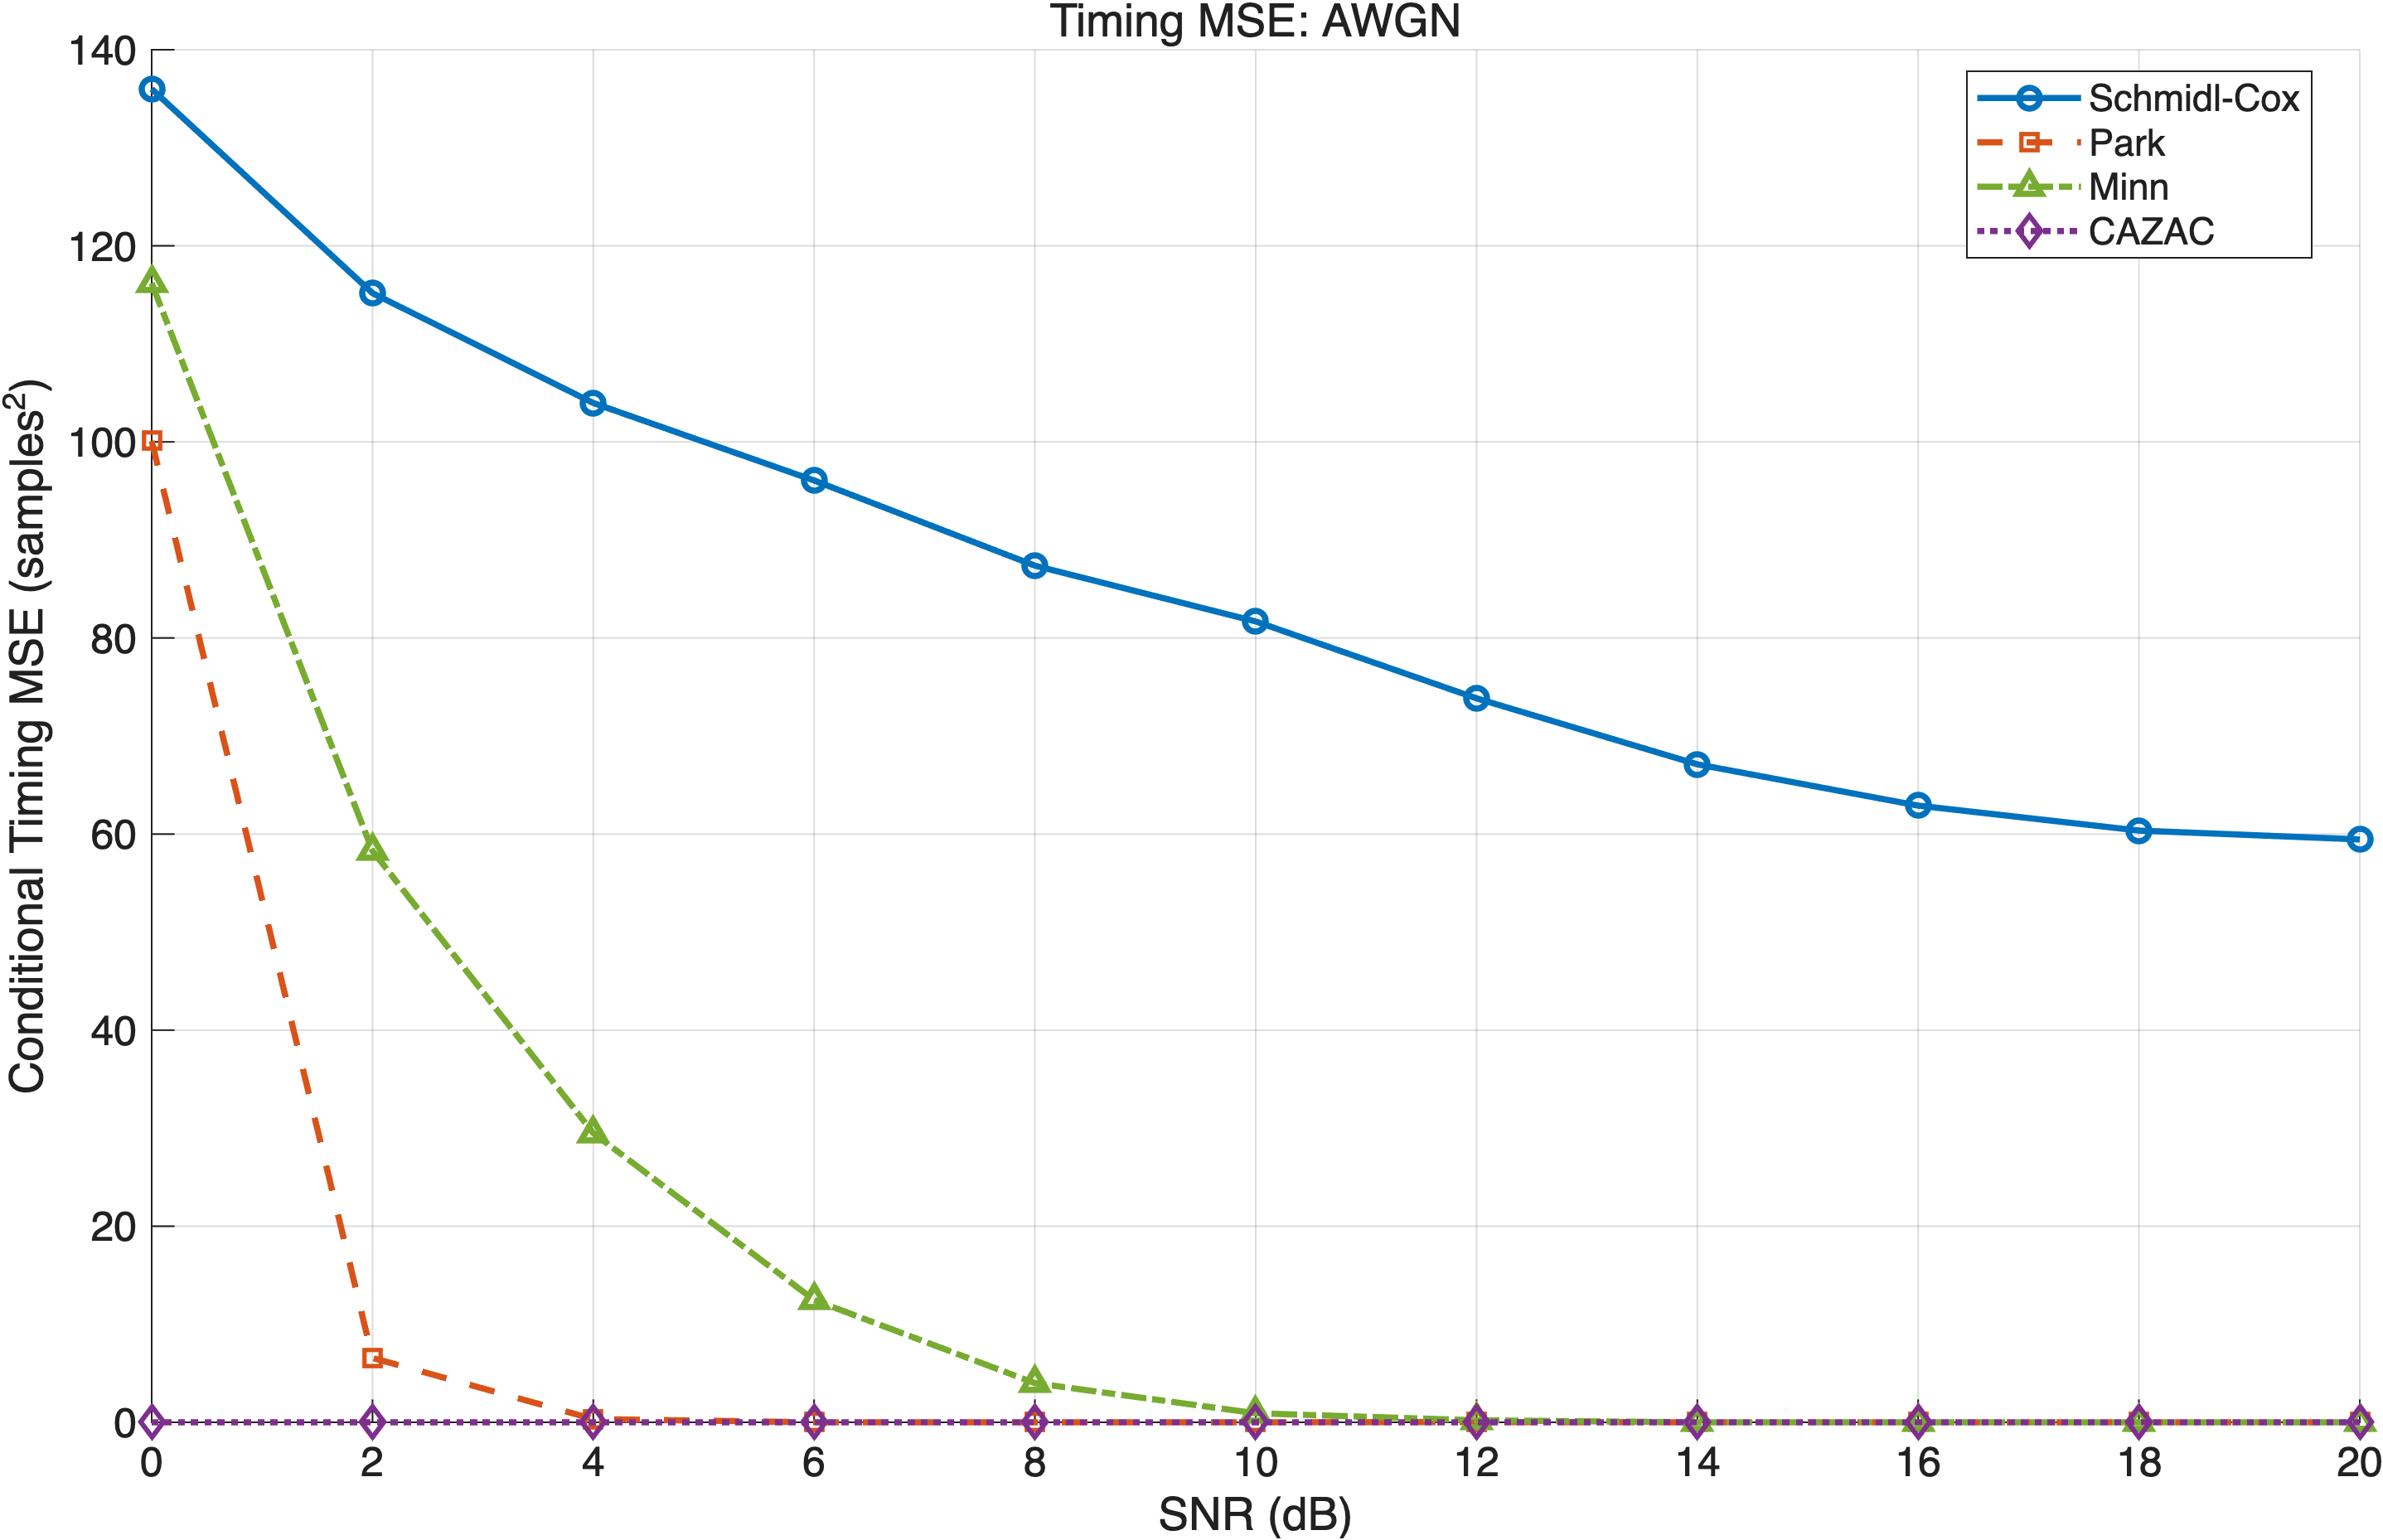
\includegraphics[width=0.84\linewidth,height=0.36\textheight,keepaspectratio]{figures/ch4/exp07_awgn_mse.png}\par\smallskip
{\small (a) AWGN}\par\medskip
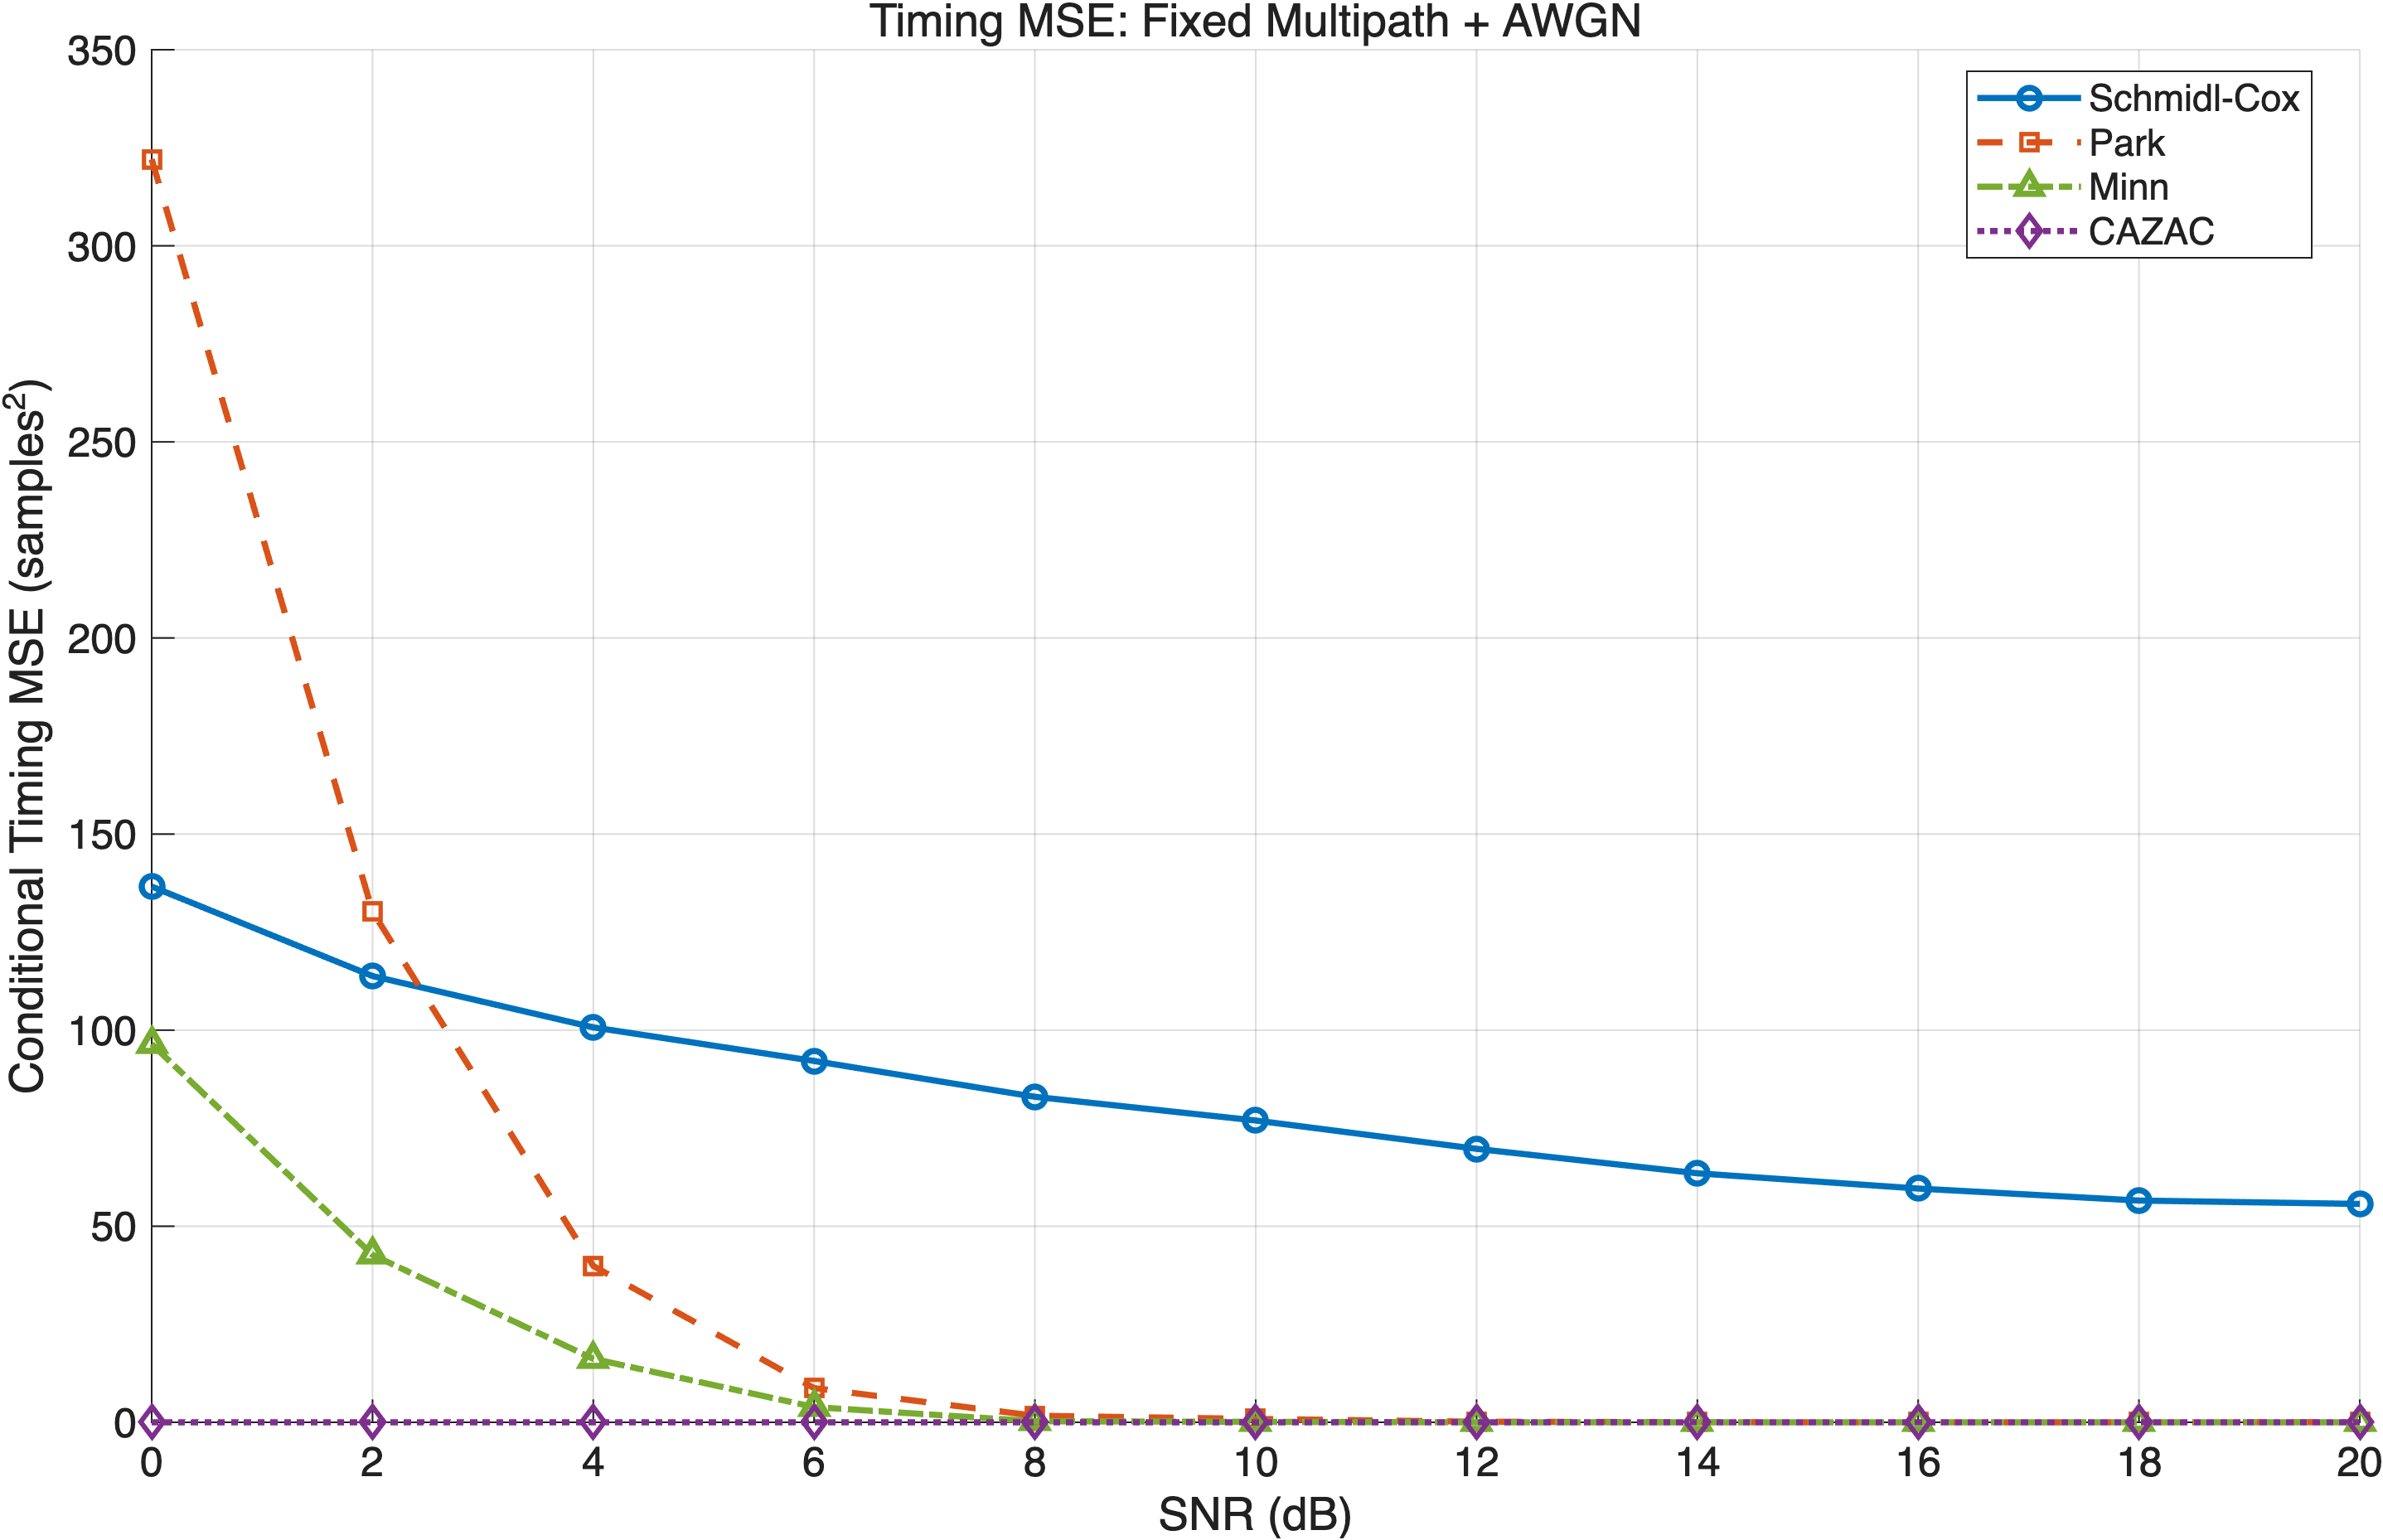
\includegraphics[width=0.84\linewidth,height=0.36\textheight,keepaspectratio]{figures/ch4/exp07_multipath_mse.png}\par\smallskip
{\small (b) Fixed multipath with AWGN}
\caption{EXP07: empirical timing MSE over the full SNR grid.}
\label{fig:ch4_mse}
\end{figure}

\begin{figure}[p]
\centering
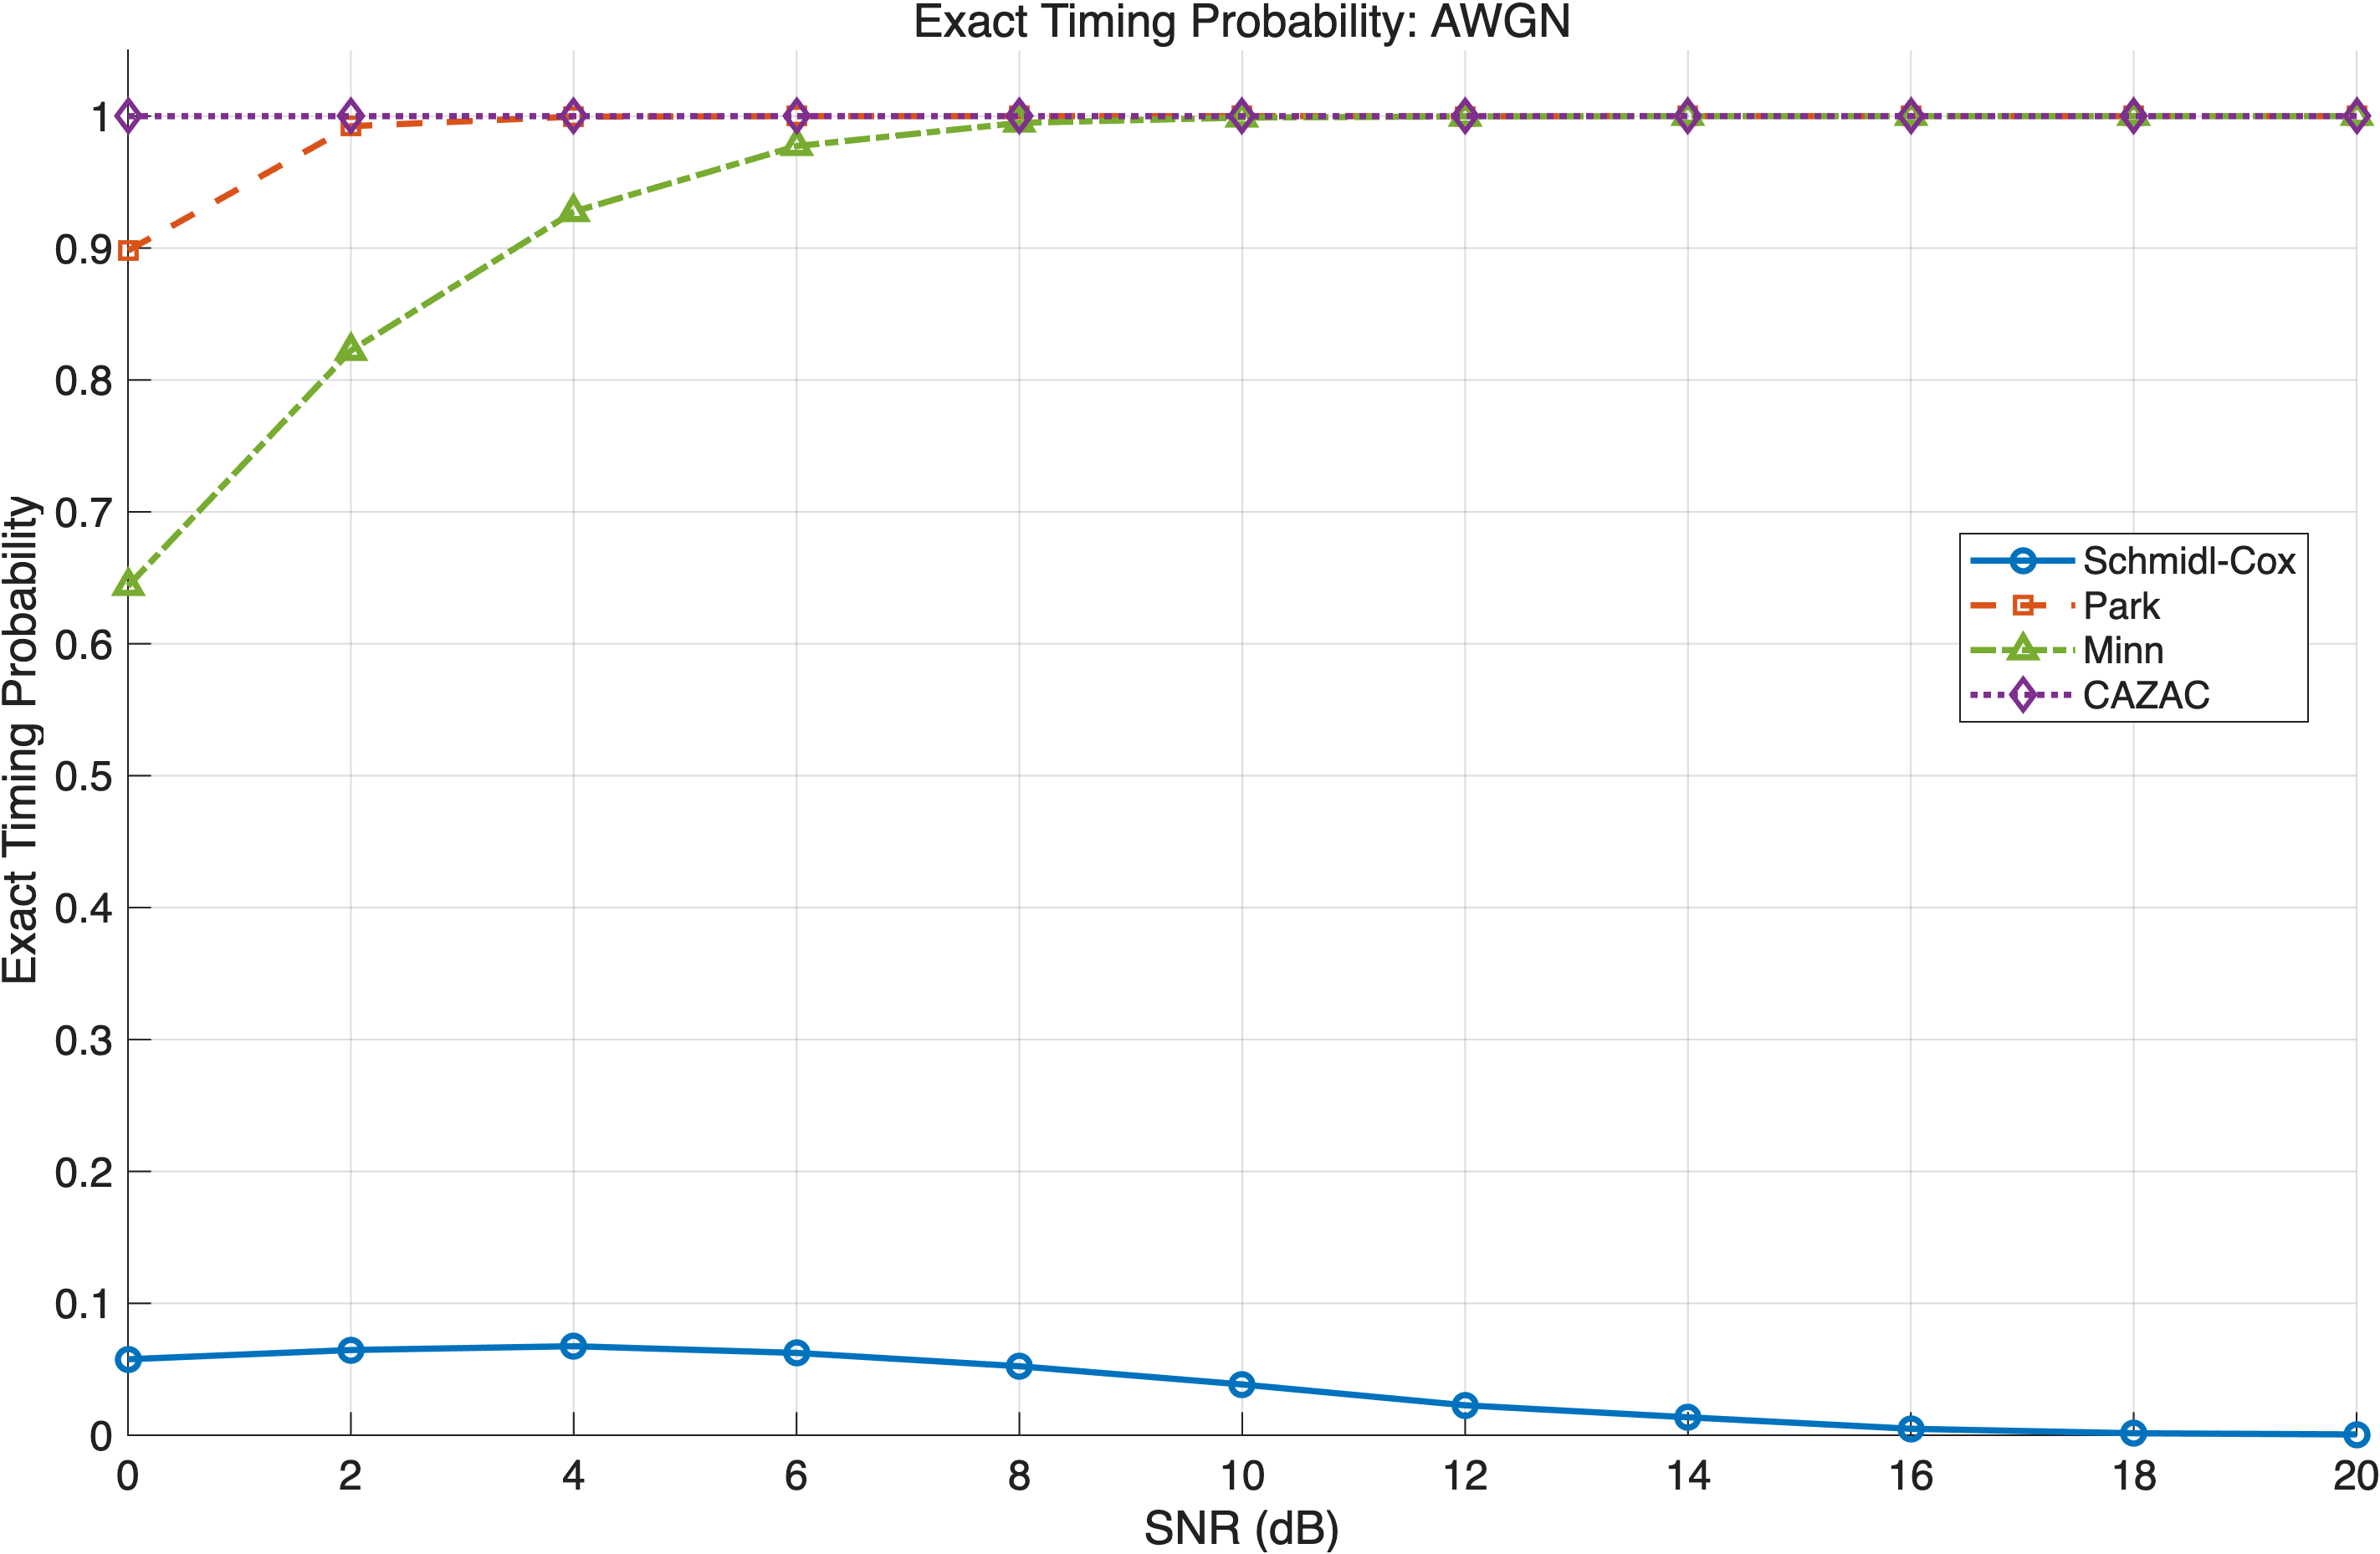
\includegraphics[width=0.84\linewidth,height=0.36\textheight,keepaspectratio]{figures/ch4/exp07_awgn_exact.png}\par\smallskip
{\small (a) AWGN}\par\medskip
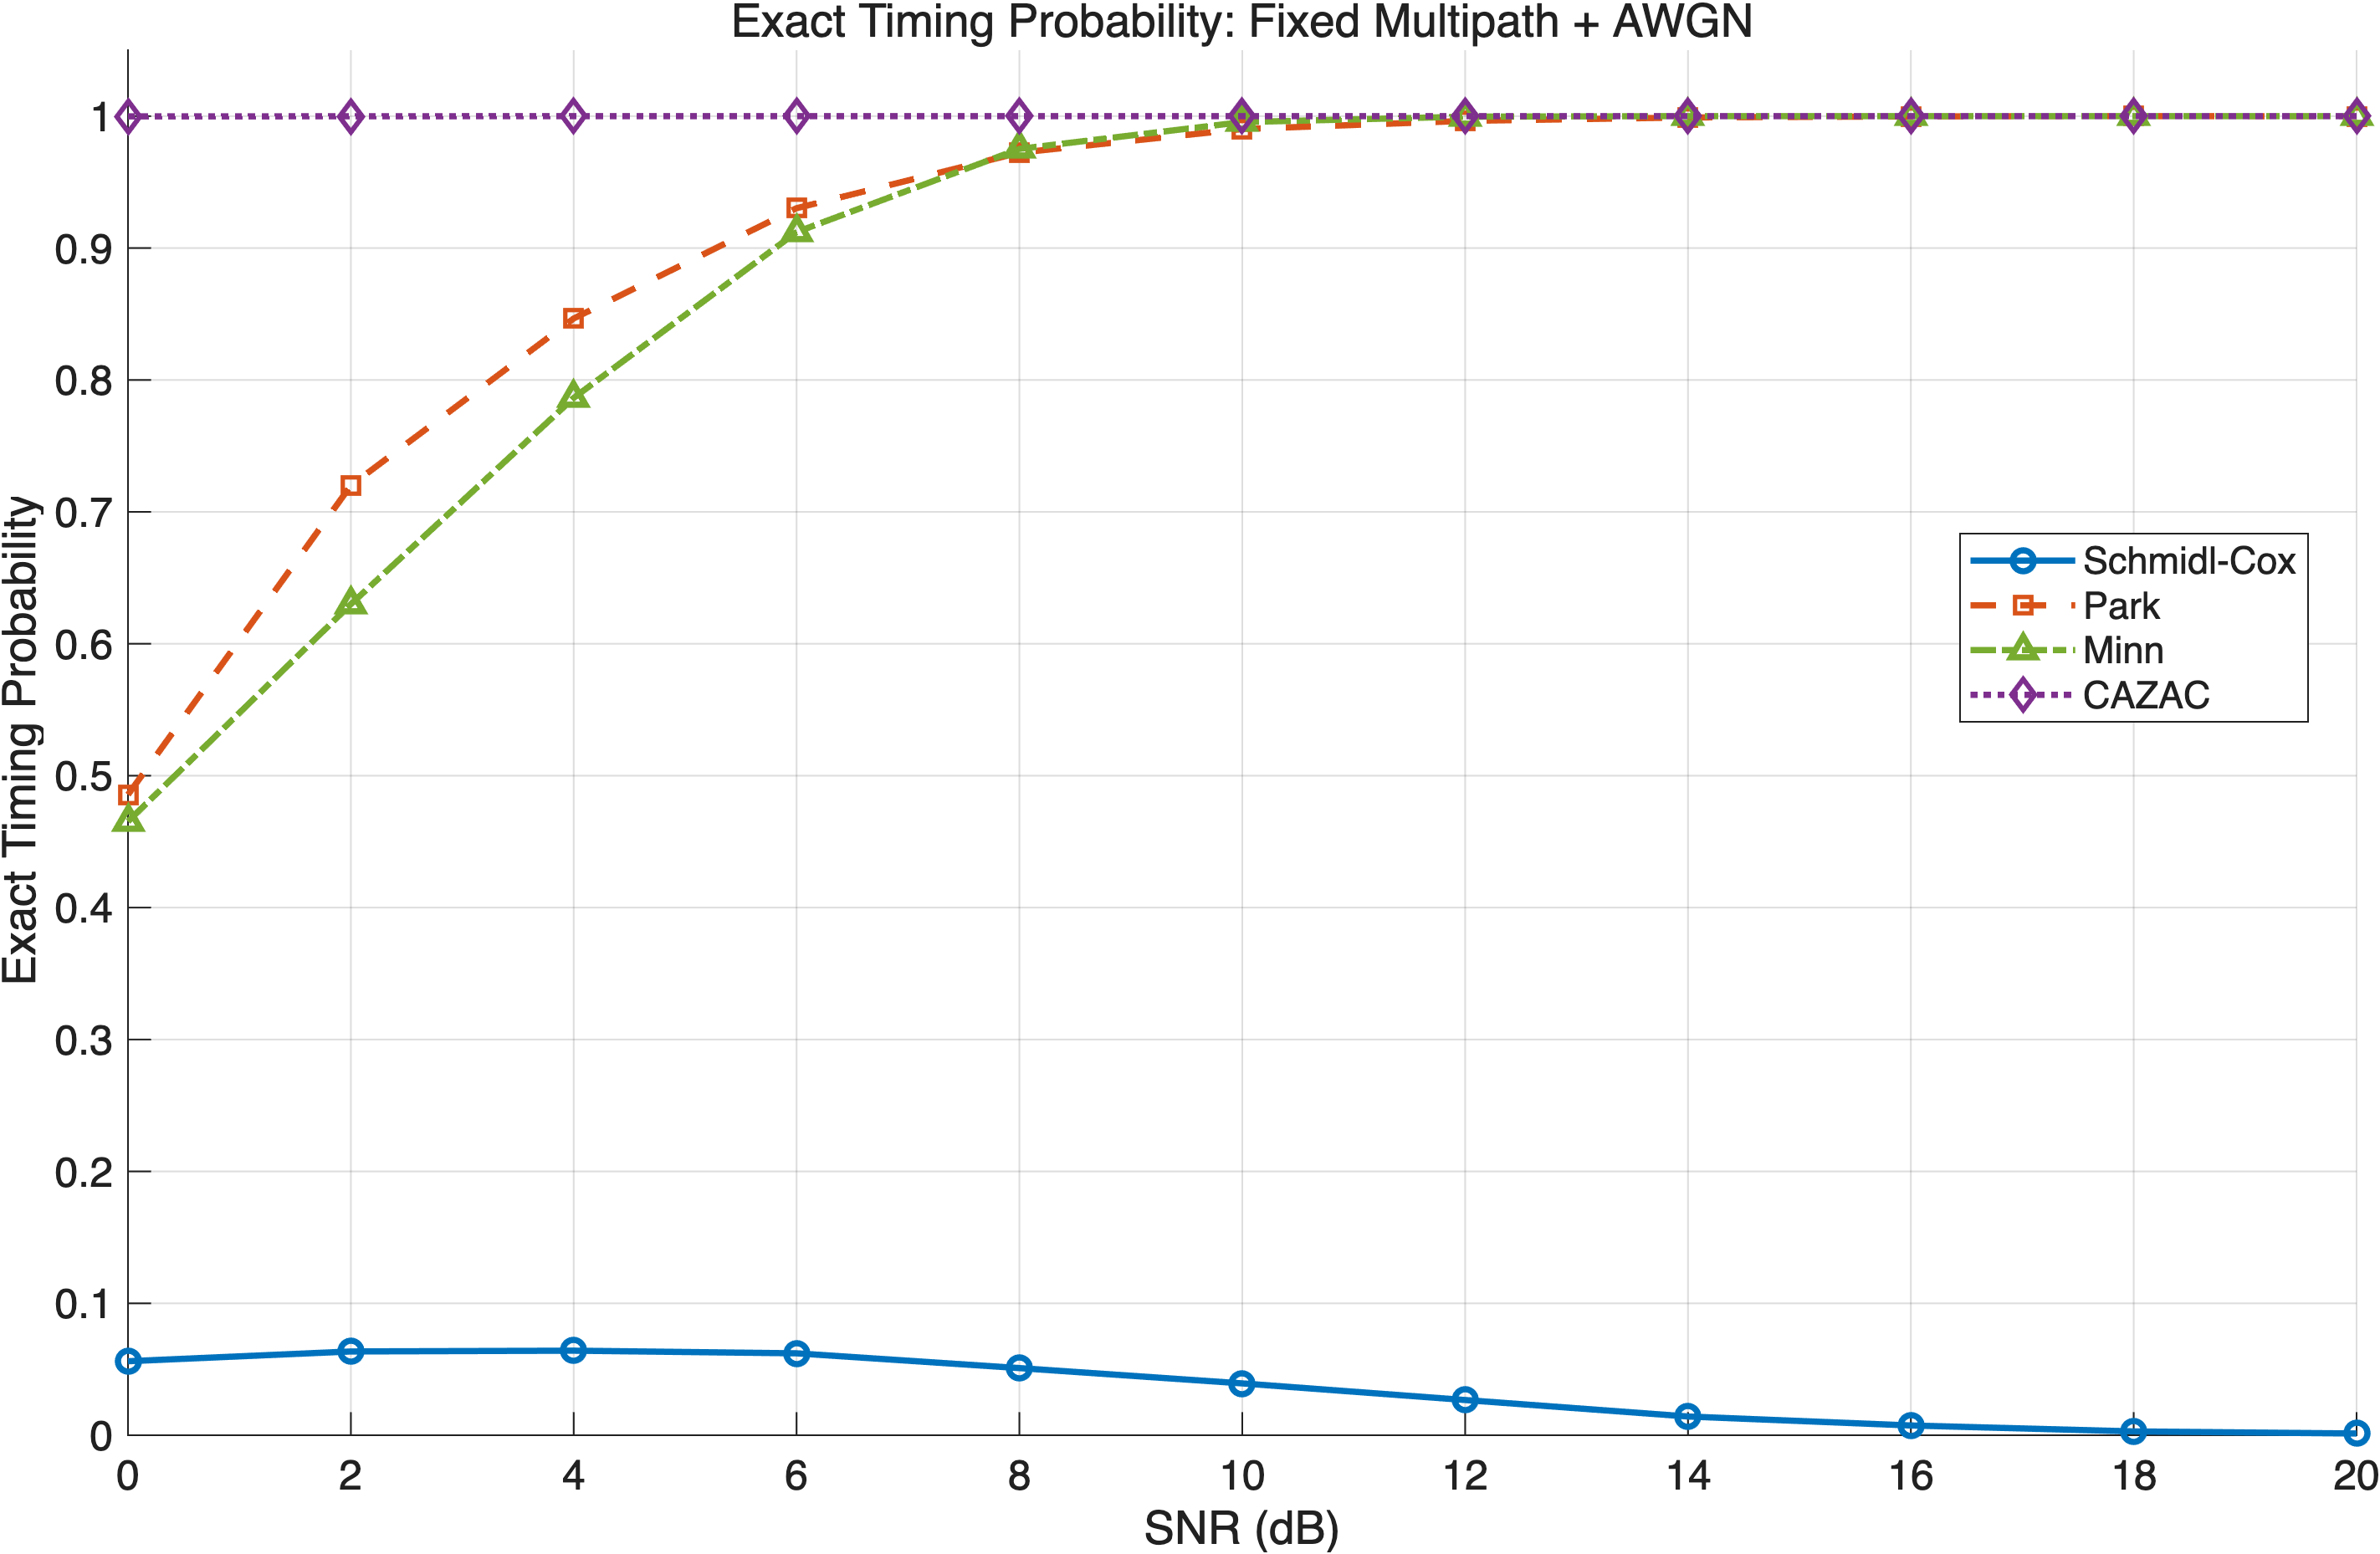
\includegraphics[width=0.84\linewidth,height=0.36\textheight,keepaspectratio]{figures/ch4/exp07_multipath_exact.png}\par\smallskip
{\small (b) Fixed multipath with AWGN}
\caption{EXP07: empirical exact-timing probability over the full SNR grid.}
\label{fig:ch4_exact}
\end{figure}

\begin{figure}[p]
\centering
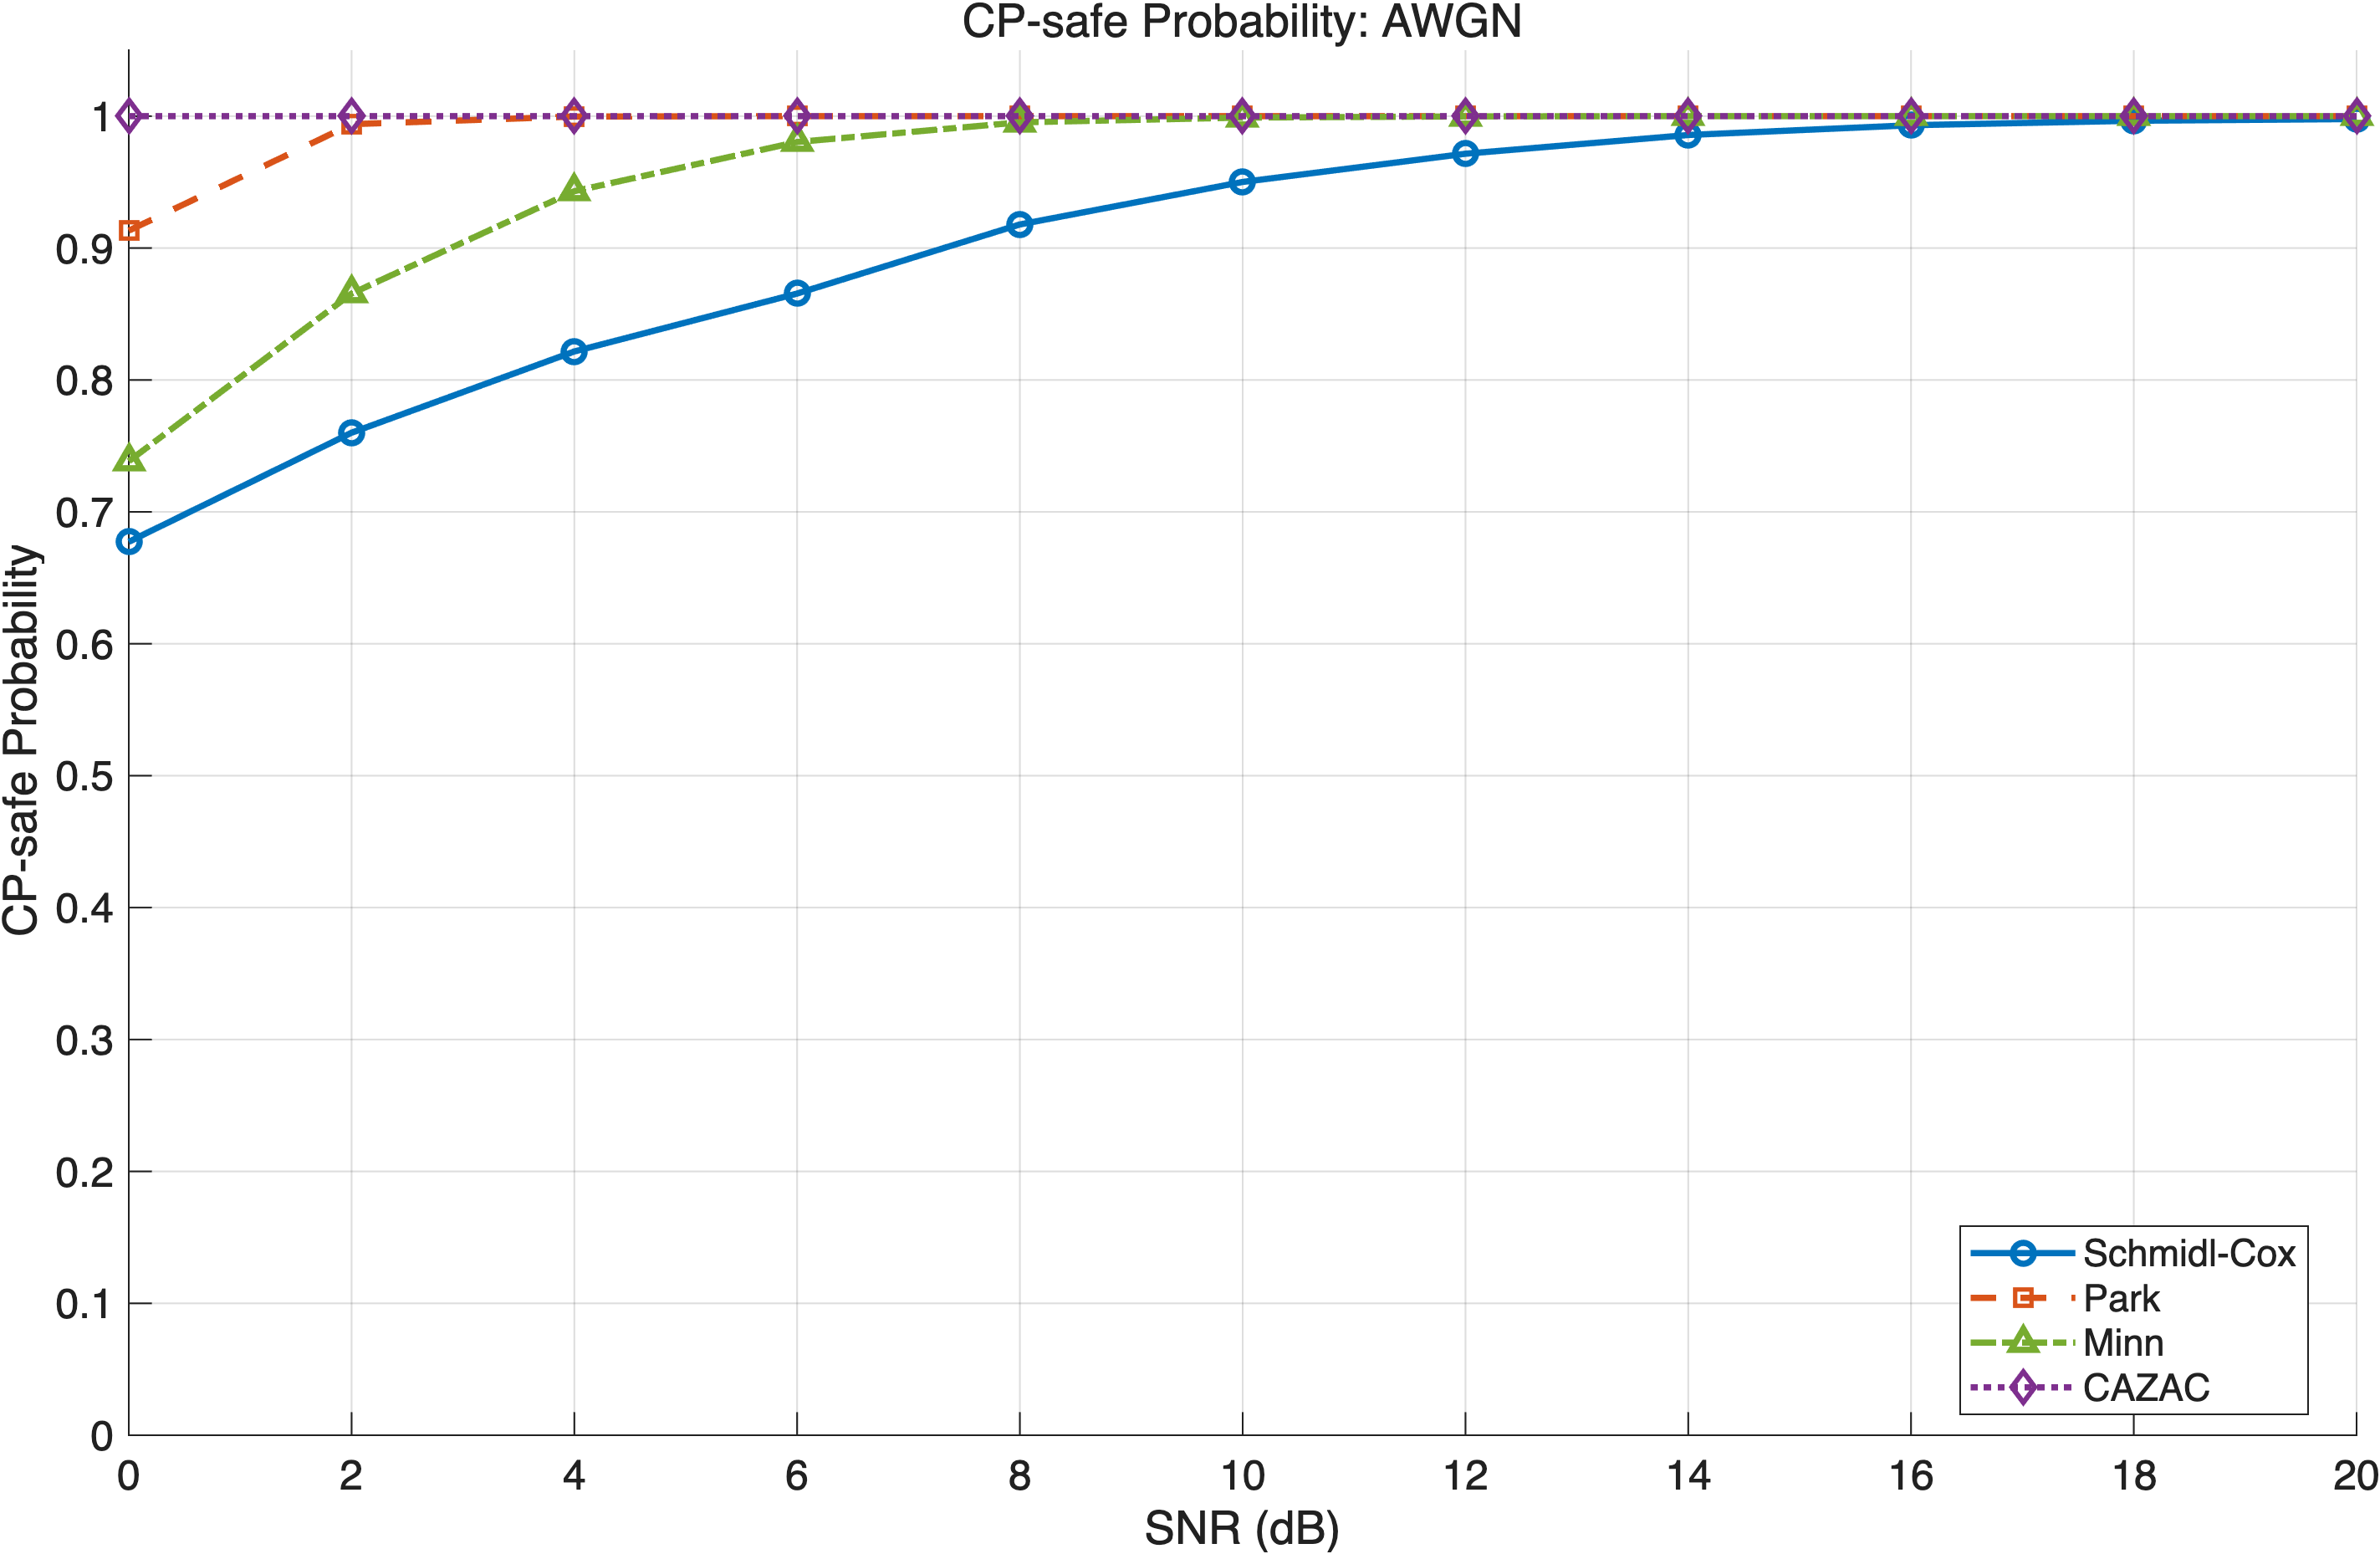
\includegraphics[width=0.84\linewidth,height=0.36\textheight,keepaspectratio]{figures/ch4/exp07_awgn_cpsafe.png}\par\smallskip
{\small (a) AWGN}\par\medskip
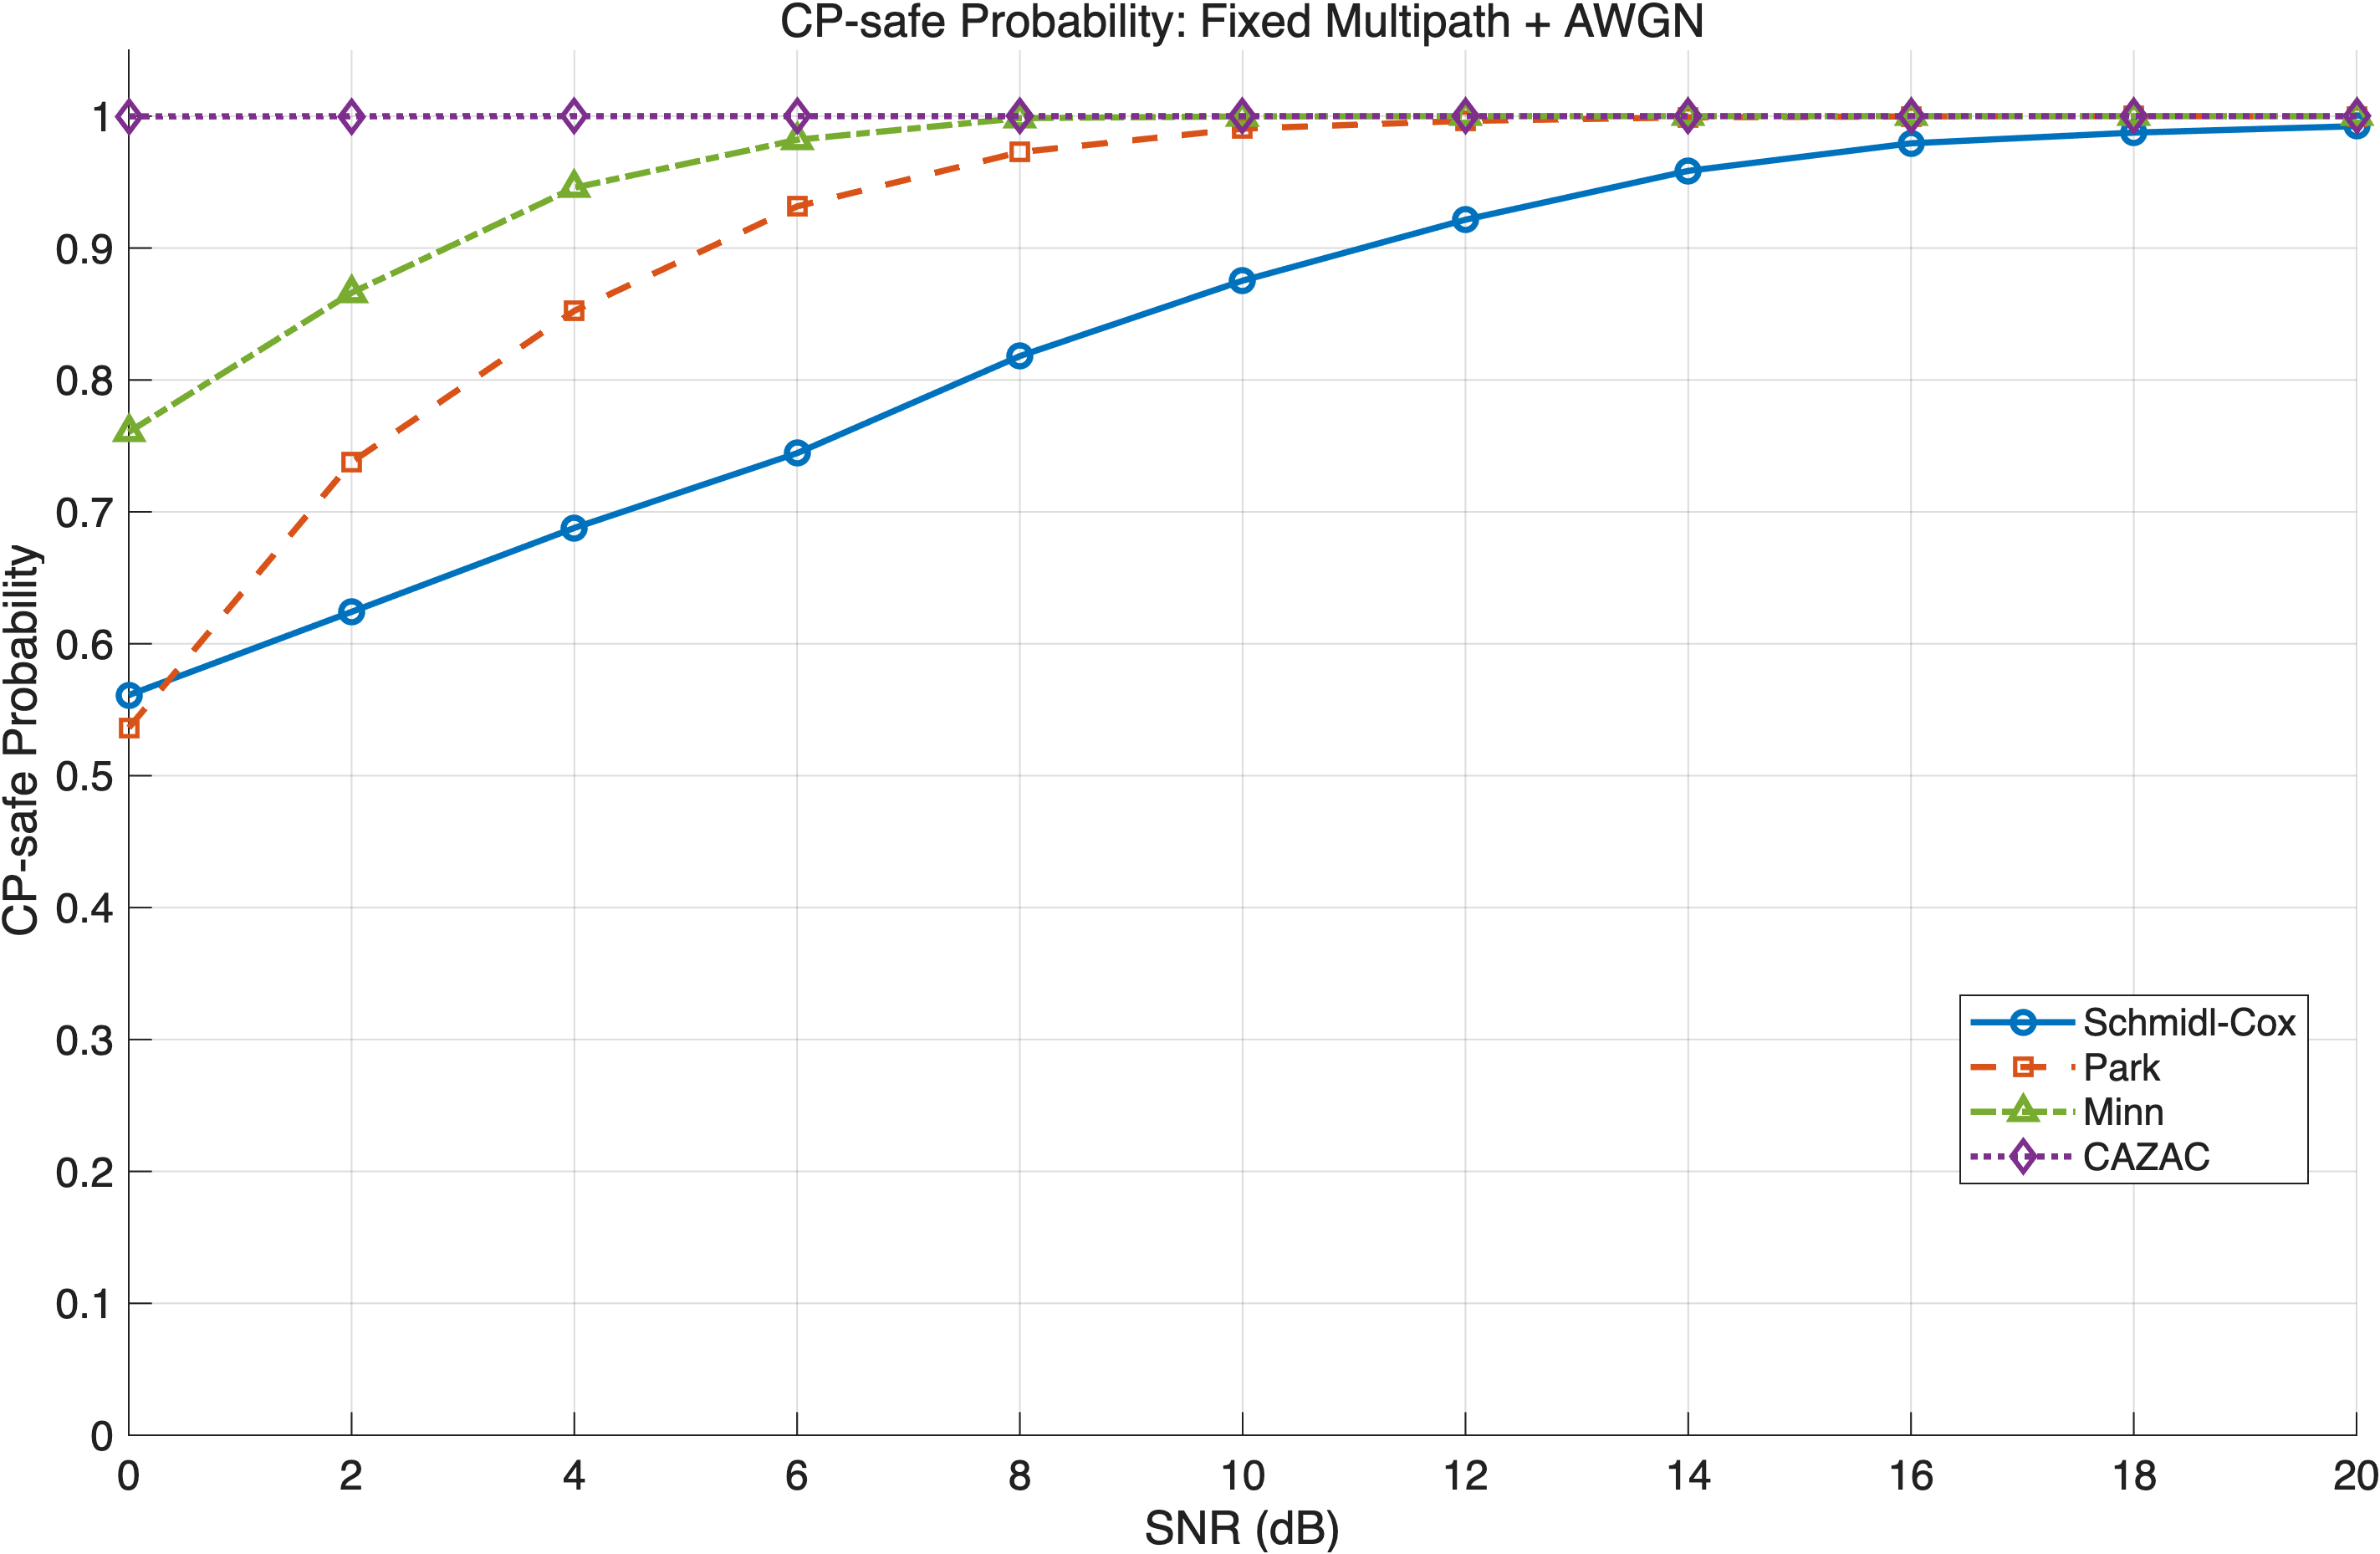
\includegraphics[width=0.84\linewidth,height=0.36\textheight,keepaspectratio]{figures/ch4/exp07_multipath_cpsafe.png}\par\smallskip
{\small (b) Fixed multipath with AWGN}
\caption{EXP07: empirical CP-safe probability over the full SNR grid. The safe intervals are $[-16,0]$ and $[-14,0]$ for (a) and (b), respectively.}
\label{fig:ch4_cpsafe}
\end{figure}

\subsection{Performance in AWGN}
At 0 dB, CAZAC has zero observed timing errors, Park achieves an exact probability of 0.8981, Minn 0.6438 and S\&C 0.0576. The corresponding MSE values for Park, Minn and S\&C are 100.1021, 116.1906 and 135.9962. As SNR increases, Park and Minn reduce their MSE rapidly; at 10 dB, Park has zero observed errors while Minn has MSE 0.9218 and exact probability 0.9989. At 20 dB, all three peak-based methods have zero observed errors.

The S\&C result differs qualitatively. Its MSE decreases from 135.9962 to 59.4513 between 0 and 20 dB, while CP-safe probability increases from 0.6773 to 0.9978. Yet the exact probability decreases to 0.0006 at 20 dB. A more stable metric leads to a more consistently early midpoint, not a more accurate estimate of the right-hand plateau boundary. Thus the improvement in safe-window placement is not equivalent to exact boundary acquisition.

\subsection{Performance in fixed multipath}
The fixed three-tap channel changes the estimator behavior most visibly at low SNR. At 0 dB, Park's exact probability falls from 0.8981 in AWGN to 0.4856 and its MSE rises to 322.0781. Minn has slightly lower exact probability (0.4653) but substantially lower MSE (96.4519) and higher CP-safe probability (0.7605) than Park (0.5363). Its errors are more often small or early enough to remain safe. The two criteria therefore produce different rankings. Minn's CP-safe probability at this point is also higher than its own AWGN value, despite the narrower acceptance interval; this is an empirical feature of this channel and error distribution, not a general benefit of multipath.

At 10 dB, Minn records exact and CP-safe probabilities of 0.9955 and 0.9998, with MSE 0.1140. Park records 0.9902 and 0.9905, with MSE 0.8639. S\&C reaches CP-safe probability 0.8753 but remains biased early. At 20 dB, Minn and CAZAC are exact in all 10,000 trials; Park has one nonzero error. S\&C reaches 0.9924 CP-safe probability but only 0.0013 exact probability. The S\&C MSE at 20 dB is somewhat smaller than in AWGN, which should not be interpreted as greater overall robustness: the safe interval has narrowed and the CP-safe probability is lower.

CAZAC's only errors in the unified experiment occur in fixed multipath at 0 and 2 dB: two and one estimates, respectively, are late by one sample. Across all 220,000 CAZAC estimates there are three nonzero errors. This high empirical accuracy is conditional on the selected deterministic channel, known template and bounded search range, not a universal performance guarantee.

\section[Error Distributions and Bias]{Timing-Error Distributions and Bias--Variance Analysis}
\label{sec:ch4_distribution}
The summary probabilities and MSE are complemented by the empirical distributions of the stored trial-level errors. Figures~\ref{fig:ch4_sc_hist}--\ref{fig:ch4_minn_hist} show three selected conditions, with bars representing percentages of all 10,000 trials and shaded regions indicating the integer CP-safe errors. These plots are derived from the EXP07 MAT arrays, rather than from the earlier individual-estimator experiments.

\begin{figure}[!htbp]
\centering
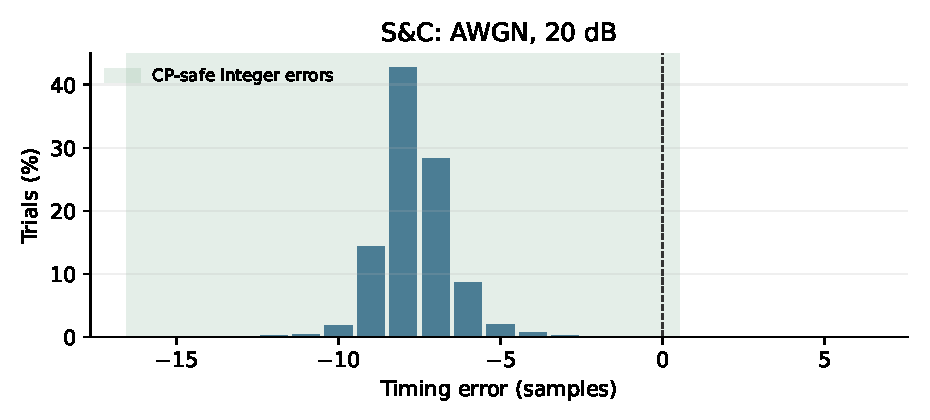
\includegraphics[width=1\linewidth]{figures/ch4/sc_awgn20_errors.pdf}
\caption{EXP07: S\&C timing-error distribution at 20 dB AWGN.}
\label{fig:ch4_sc_hist}
\end{figure}

\begin{figure}[!htbp]
\centering
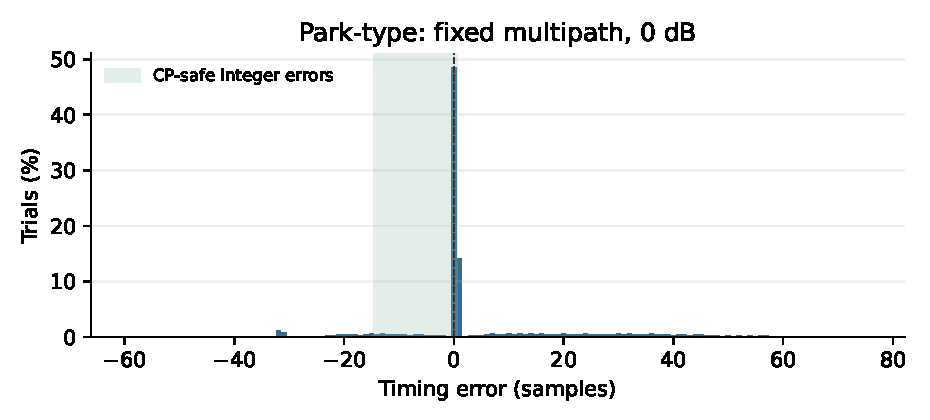
\includegraphics[width=1\linewidth]{figures/ch4/park_mp0_errors.pdf}
\caption{EXP07: Park-type timing-error distribution at 0 dB in fixed multipath.}
\label{fig:ch4_park_hist}
\end{figure}

\begin{figure}[!htbp]
\centering
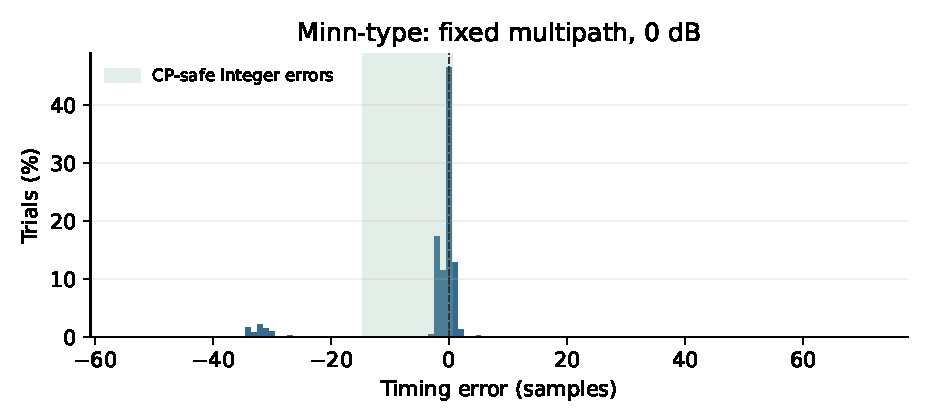
\includegraphics[width=1\linewidth]{figures/ch4/minn_mp0_errors.pdf}
\caption{EXP07: Minn-type timing-error distribution at 0 dB in fixed multipath.}
\label{fig:ch4_minn_hist}
\end{figure}

For S\&C at 20 dB AWGN, errors of $-8$ and $-7$ account for 4,278 and 2,824 trials, respectively. Only six trials give exact timing; 22 estimates are positive. The distribution is concentrated around an early offset rather than around zero. In contrast, Park at 0 dB multipath produces 4,856 exact estimates and 1,420 estimates at $+1$, with 2,508 errors of absolute magnitude at least 16 samples. Minn has 4,653 exact estimates and 1,737 at $-2$; 225 trials have error $-32$ and 905 errors have absolute magnitude at least 16. The latter secondary mode is consistent with the competing metric peak observed in the representative curves, although the stored errors alone do not prove the origin of every individual erroneous decision.

\begin{table}[htbp]
\centering
\caption{EXP07 bias--variance decomposition for selected conditions. Variance uses the denominator 10,000.}
\label{tab:ch4_biasvar}
\small
\begin{tabular}{llrrrr}
\hline
Channel, dB & Method & $\bar e$ & $\bar e^2$ & $v_K$ & MSE\\
\hline
AWGN, 20 & S\&C & $-7.6081$ & 57.8832 & 1.5681 & 59.4513\\
MP, 20 & S\&C & $-7.2907$ & 53.1543 & 2.5276 & 55.6819\\
MP, 0 & Park & 4.9677 & 24.6780 & 297.4001 & 322.0781\\
MP, 0 & Minn & $-2.9189$ & 8.5200 & 87.9319 & 96.4519\\
\hline
\end{tabular}
\end{table}

Table~\ref{tab:ch4_biasvar} decomposes MSE using the empirical identity from Section 2.9. In AWGN at 20 dB, approximately 97.36\% of S\&C MSE is squared bias; in multipath at 20 dB the proportion is approximately 95.46\%. The high-SNR limitation is systematic rather than predominantly random. By contrast, at 0 dB multipath, the variance term accounts for about 92.34\% of Park MSE and 91.17\% of Minn MSE. Large errors strongly influence the squared-error criterion even when many estimates are exact.

Rare errors also explain some apparent irregularities at high SNR. For example, Minn at 10 dB AWGN has nine errors of $-32$ and two of $+1$ among 10,000 trials. The nine large errors contribute $9(32)^2/10000=0.9216$ of its MSE of 0.9218. Park at 20 dB multipath has one error of $+19$, producing the entire MSE of 0.0361 despite 9,999 exact estimates. Its MSE was zero at 18 dB; the increase at the next tested SNR should not be interpreted as evidence of systematic deterioration. The empirical curve is sensitive to rare events and finite simulation size.

\section[Statistical Interpretation]{Statistical Interpretation and Robustness}
\label{sec:ch4_statistical}
With 10,000 trials in a condition, probability estimates have a resolution of 0.0001. Under independent trials at a fixed condition, the binomial standard error is $\sqrt{p(1-p)/10000}$, at most 0.005. For example, the plug-in standard errors of Park and Minn exact probability at 0 dB multipath are both close to 0.005. Since the methods share trial scenarios, comparisons between them should not be treated as tests of two independent proportions. This chapter uses descriptive comparisons rather than claiming formal statistical significance from separate marginal standard errors.

When no nonexact estimates are observed in 10,000 trials, a one-sided 95\% binomial upper bound on the nonexact probability is $1-0.05^{1/10000}\approx 0.000300$, assuming independent trials with a common probability for that condition. This illustrates the finite-sample uncertainty even when the reported exact probability equals one. The bound is per condition and is not a simultaneous guarantee over the full SNR grid. All reported zero MSE and zero failure values are empirical observations.

The primary comparison identifies three distinct patterns: plateau-induced bias for S\&C, noise- and channel-sensitive peak selection for Park and Minn, and very reliable known-template matching for CAZAC in the tested model. Identical transmitted energy and a common candidate support make the comparison more controlled, but do not equalize the information used by each estimator. The results characterize the four selected implementations under the stated simulation conditions. They do not establish that a specific algorithm is universally optimal or that its performance is unchanged under other channel profiles, frequency offsets or fractional delays.

\section{Chapter Summary}
EXP01 and EXP02 verify the OFDM processing model and distinguish phase rotation from loss of the circular-convolution structure. EXP07 shows that exact timing, CP-safe timing and MSE describe distinct properties. A method may place most windows within the safe interval while retaining systematic bias, or achieve a high exact probability while suffering large MSE due to rare errors. Chapter 5 uses EXP08 to examine their consequences for data detection.


% Chapter 5: BER Performance and Discussion
\chapter[BER Performance and Discussion]{End-to-End BER Performance and Discussion}
\label{chap:ber_results}

Chapter 4 established that the four timing estimators differ in exact-boundary accuracy, CP-safe window placement and the distribution of timing errors. This chapter examines the consequences of those errors for data detection, addressing the fourth research question. Unlike the imposed displacements in EXP02, the FFT-window positions in EXP08 are determined by the actual timing estimates. The comparison also considers computational requirements and the limitations of the simulation model.

\section[EXP08 Evaluation]{End-to-End Evaluation in EXP08}
EXP08 retains the frame structure, delay distribution, candidate search interval, channels and received active-frame SNR grid of EXP07, but uses its own random seed (2049) and newly generated data frames. Thus the timing observations used in this chapter come from EXP08, not from a trial-by-trial combination of EXP07 timing errors and EXP08 bit errors. The three receiver configurations defined in Section~3.8 are evaluated on the same received frame: perfect timing with the physical channel response, estimated timing with the physical channel response, and estimated timing with oracle phase compensation. The last two cases use exactly the same FFT window.

There are 88 algorithm--channel--SNR conditions and 10,000 frames per condition, giving 880,000 timing-estimation trials and 2,640,000 receiver evaluations. All timing estimates and receiver evaluations are valid in the saved outputs. Each receiver-specific condition therefore contains 1,280,000 decoded bits, with no observed lost bits. The cumulative count is 337,920,000 decoded bits across receiver evaluations; it is not a count of independent bit observations. Because no frames are lost, conditional BER and bit-delivery failure ratio coincide in this experiment. A valid decoded frame may nevertheless contain incorrect bits.

All empirical BER values reported here use the actual bit-error counts. The original MATLAB logarithmic plots display zero-error observations at $1/1{,}280{,}000=7.8125\times10^{-7}$ with downward triangles. This is a graphical convention, not a physical error floor, a positive observed BER or a confidence bound. In particular, the marker for one observed error may have the same vertical coordinate as a zero-error marker.

\section[Perfect-Timing Reference]{Perfect-Timing BER Reference}
\label{sec:ch5perfect}
Figure~\ref{fig:ch5perfect} shows the performance when the useful data-symbol boundary is known. This reference removes synchronization error while retaining channel effects, noise and the same data processing as the estimated-timing receivers.

\begin{figure}[!htbp]
\centering
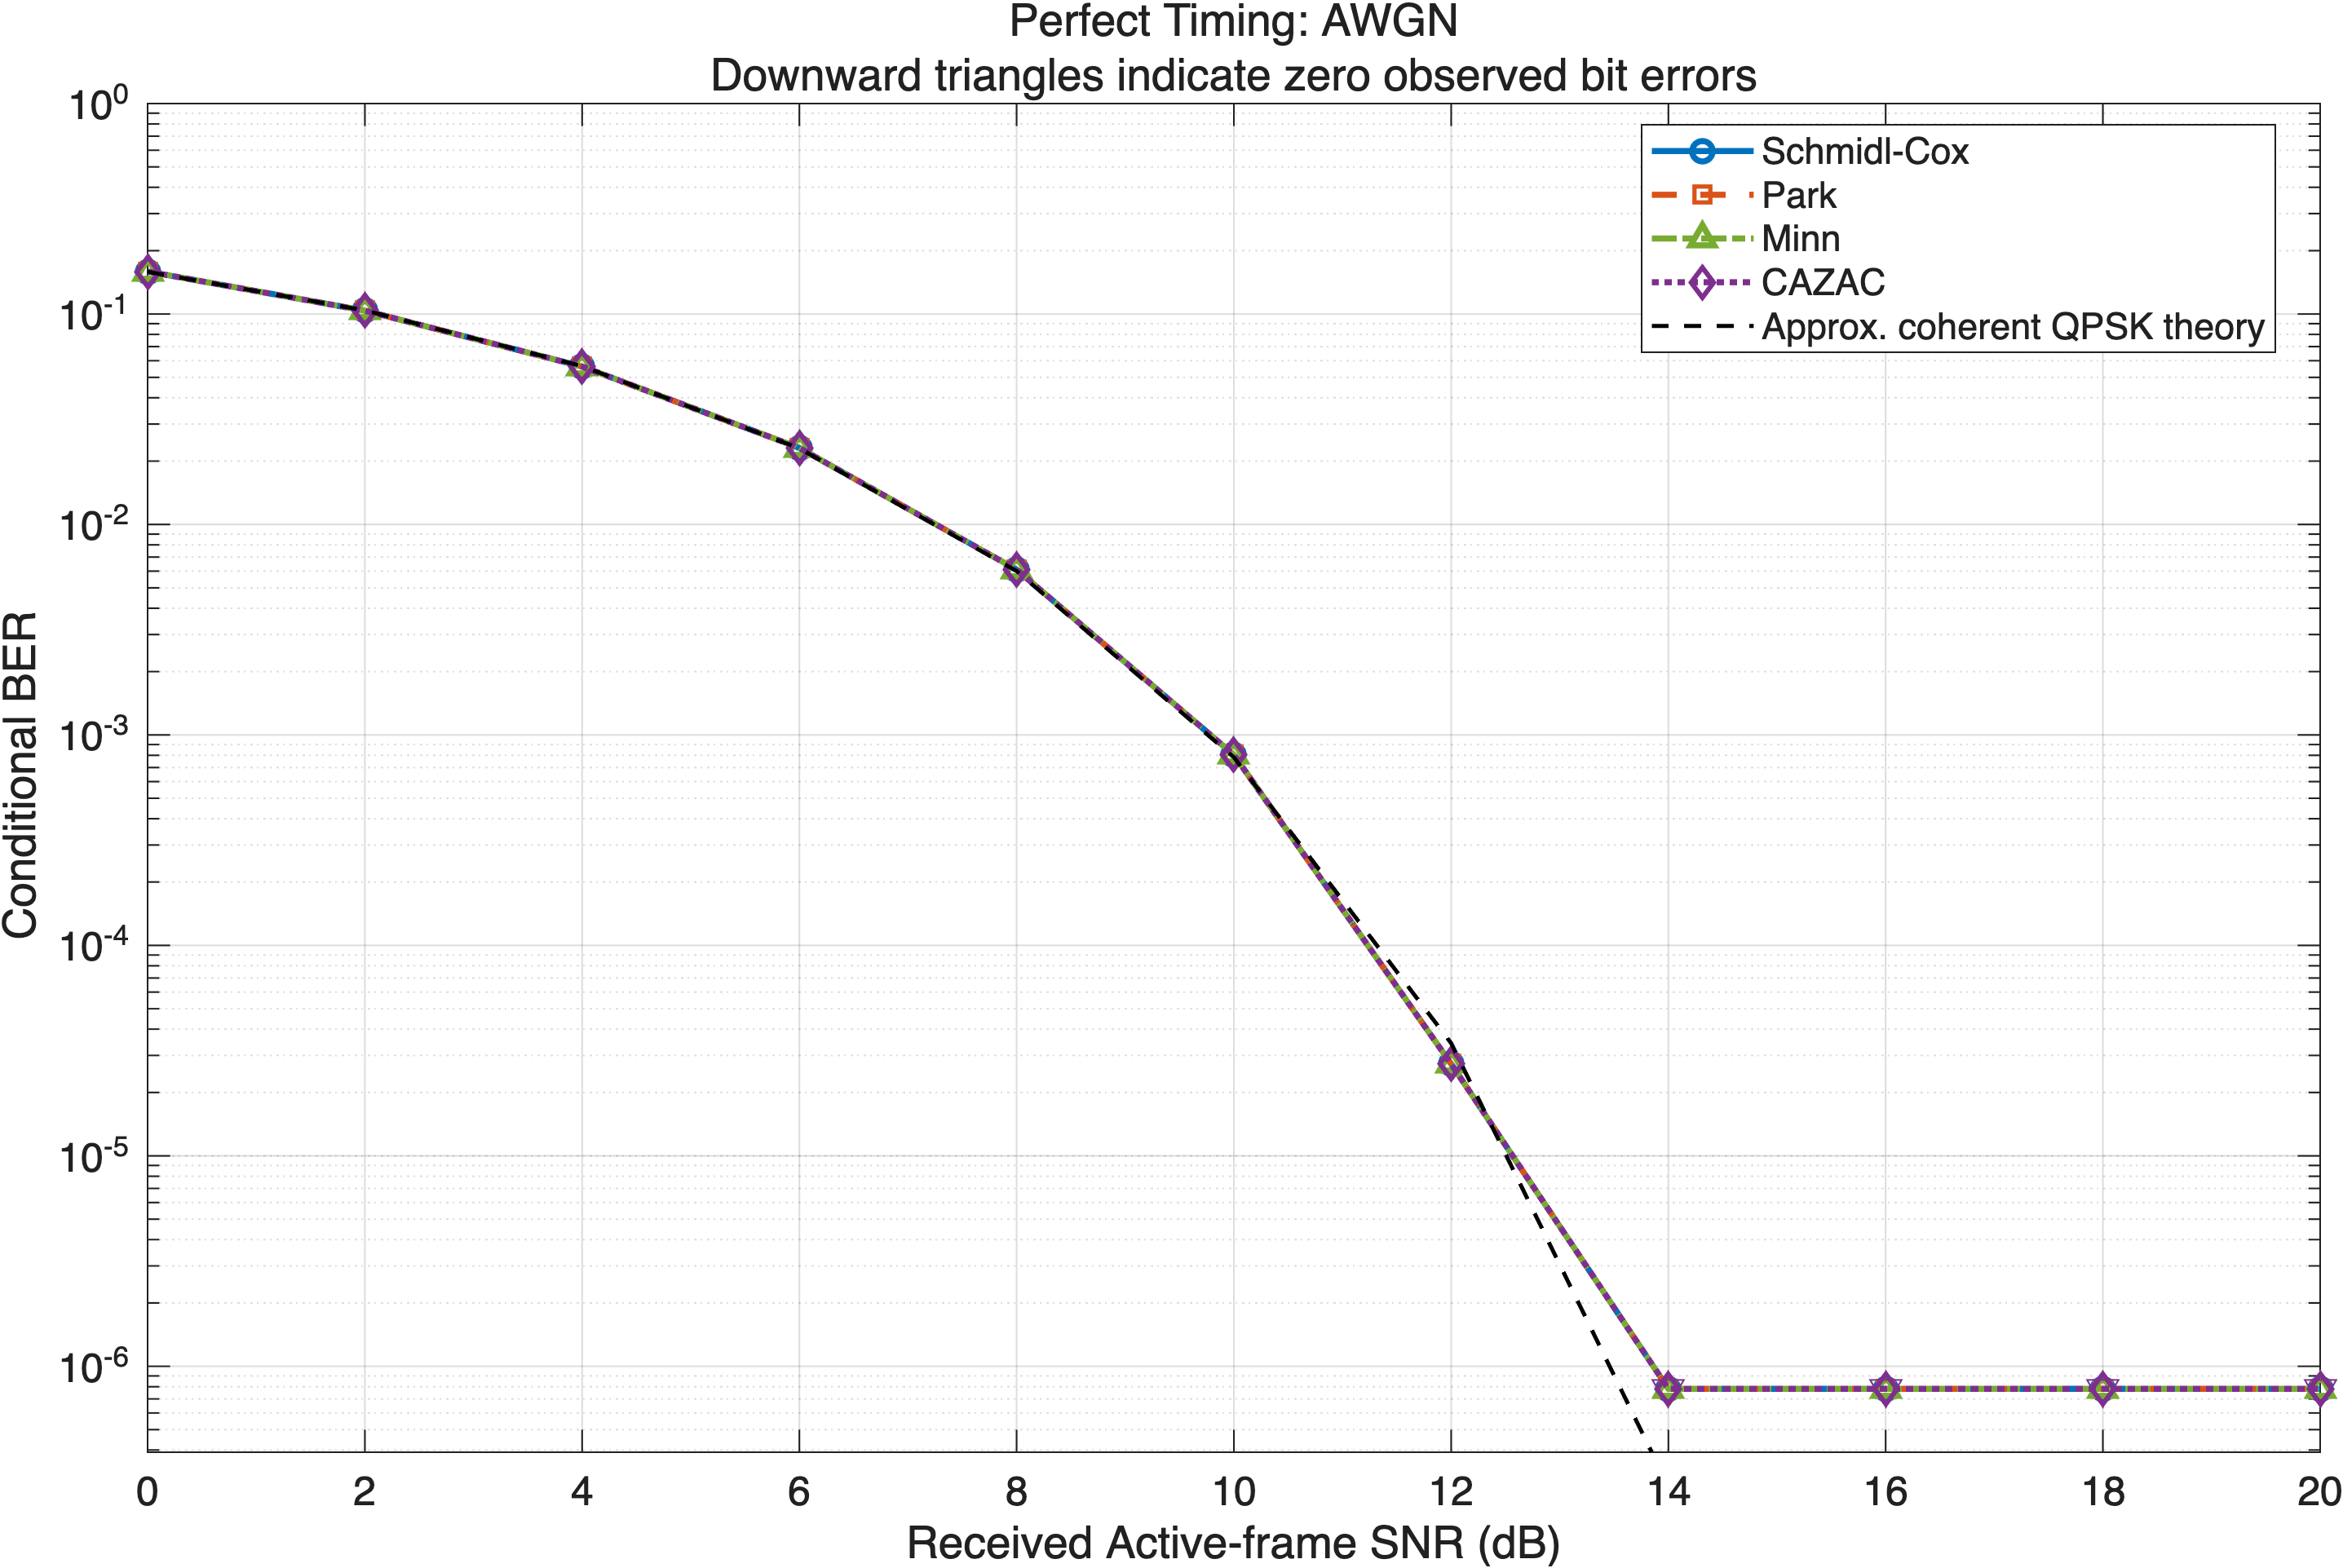
\includegraphics[width=0.90\textwidth,height=0.30\textheight,keepaspectratio]{figures/ch5/exp08_awgn_ber_perfect.png}\par
{\small (a) AWGN}\par\medskip
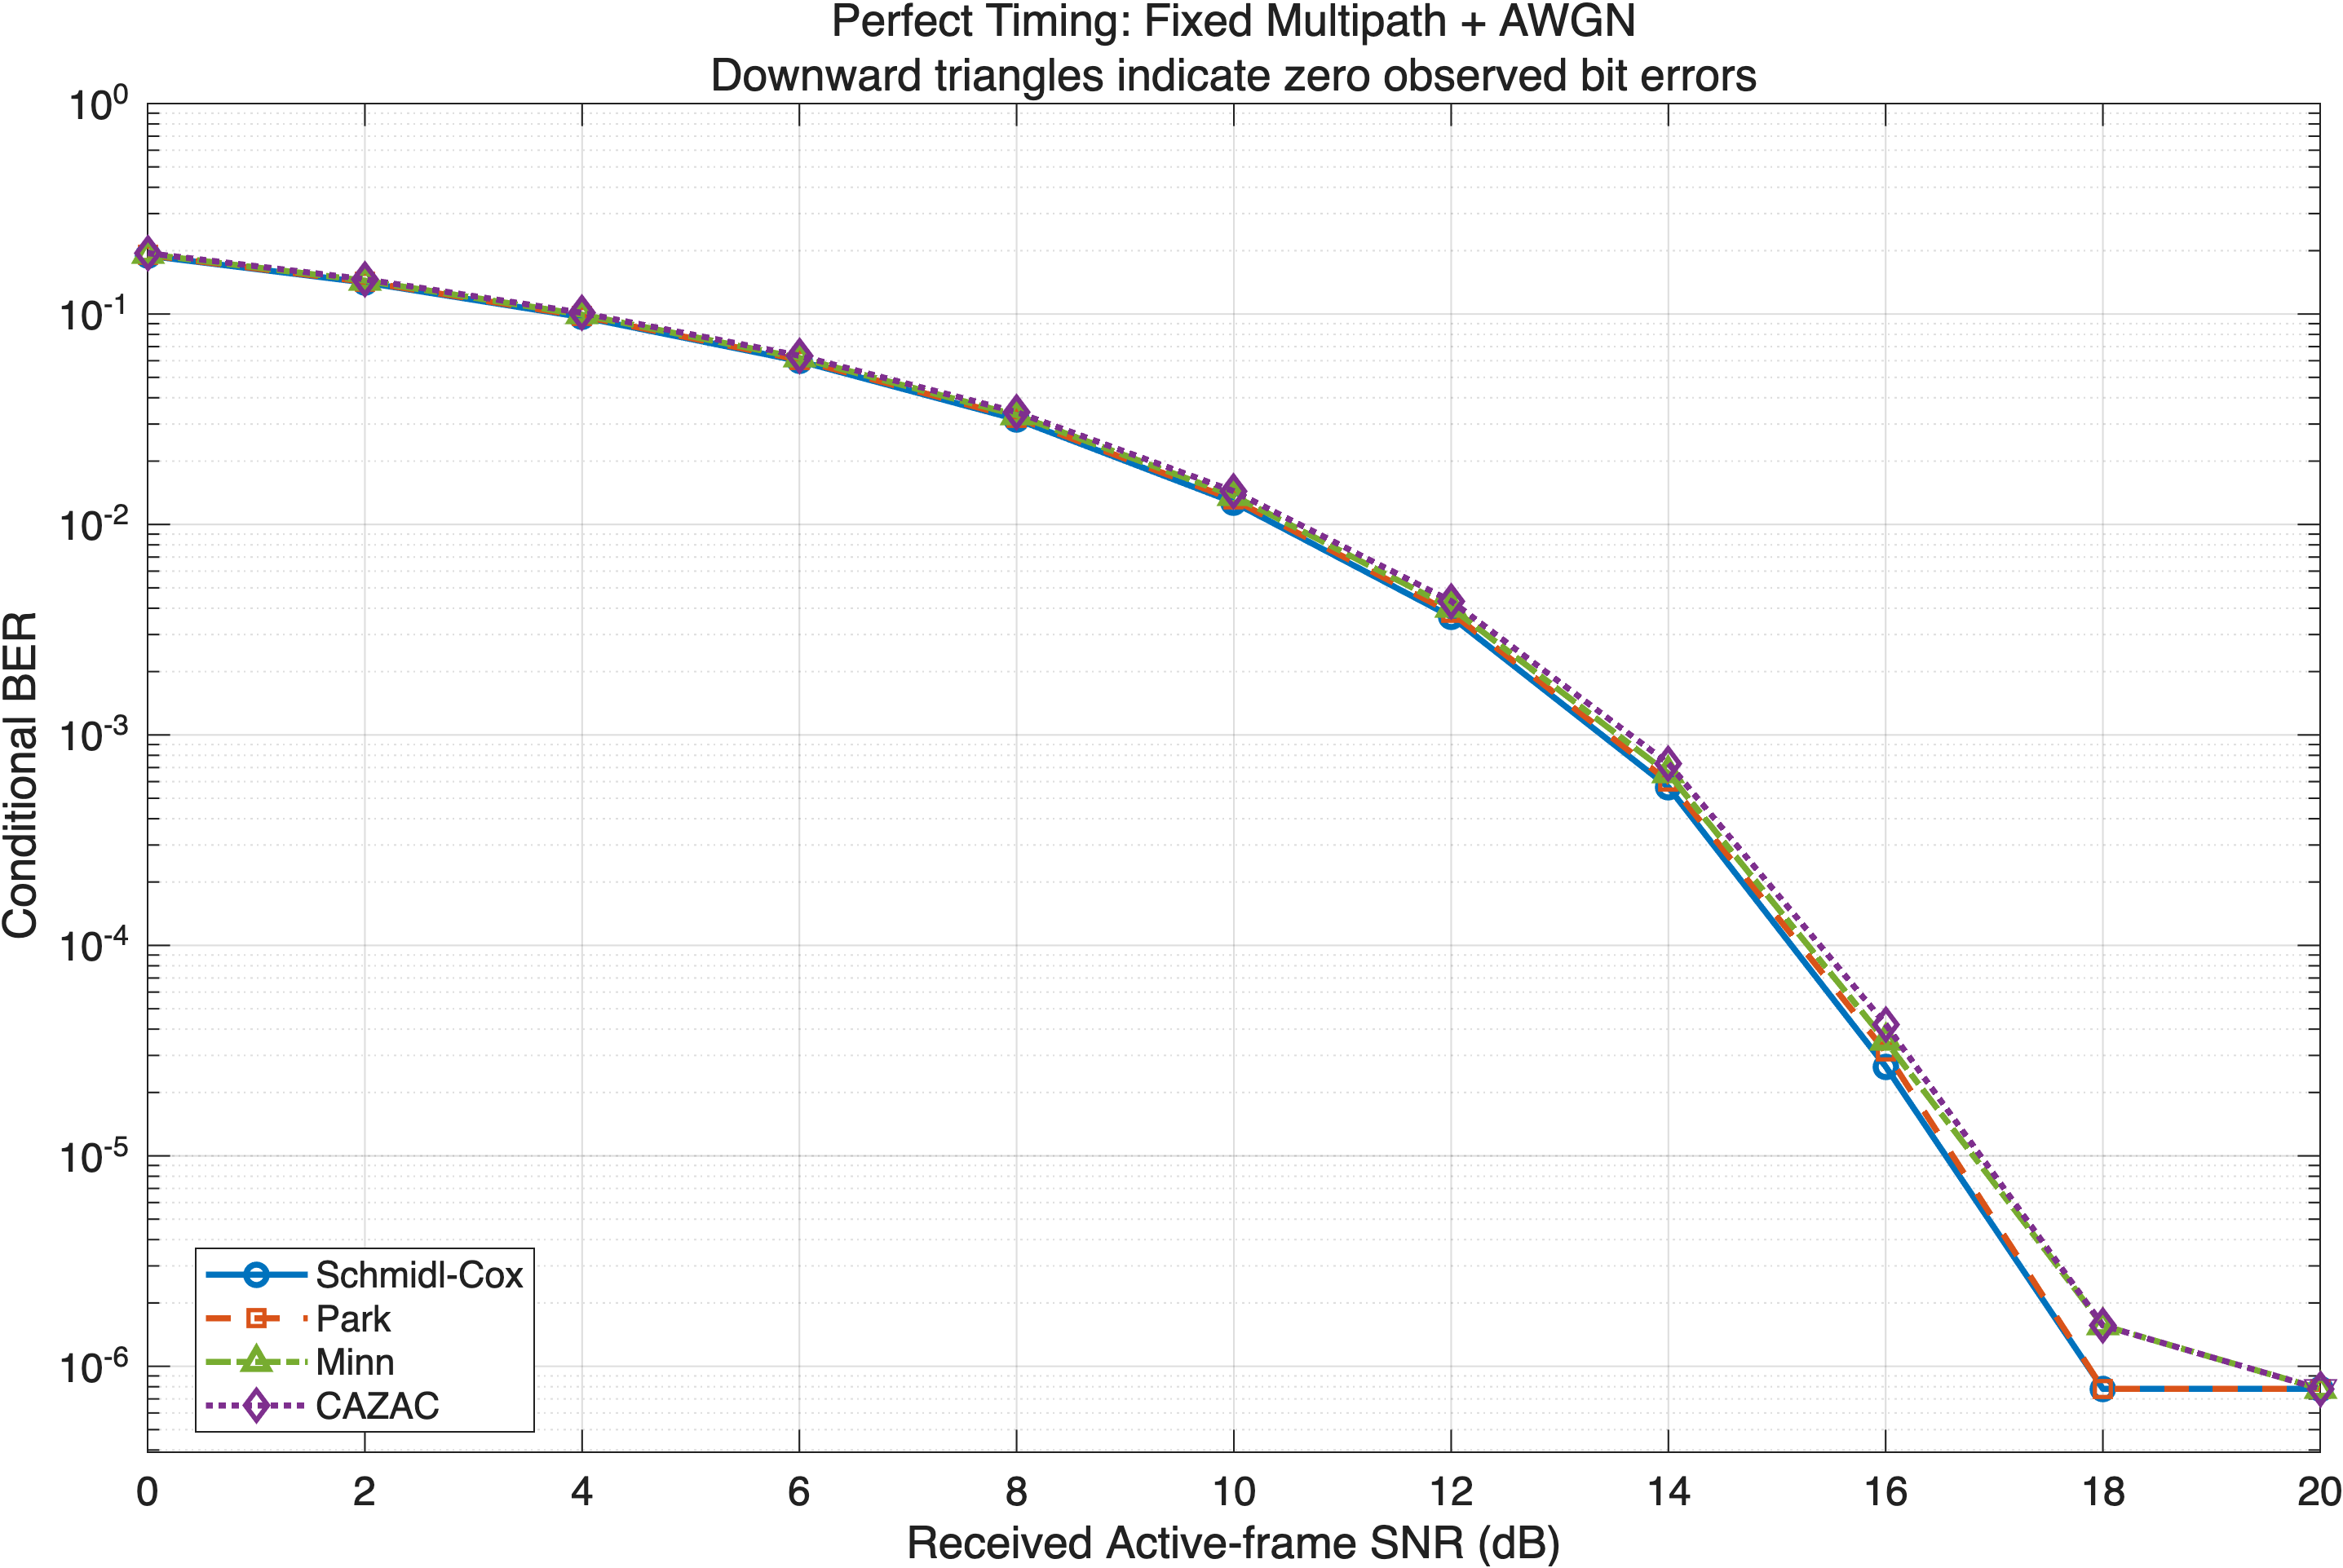
\includegraphics[width=0.90\textwidth,height=0.30\textheight,keepaspectratio]{figures/ch5/exp08_multipath_ber_perfect.png}\par
{\small (b) Fixed multipath with AWGN}
\caption[EXP08: perfect-timing BER.]{EXP08: BER with perfect timing. Downward triangles denote zero observed bit errors.}
\label{fig:ch5perfect}
\end{figure}

In AWGN, all four perfect-timing curves coincide. For a given trial, the same data vector and base noise are used, and every training and data symbol has the same CP-inclusive energy. The received active-frame power is therefore one in AWGN, independently of the preamble design. At 0 dB the common reference records 203,729 bit errors (BER 0.1591633); at 10 dB it records 1,029 errors (BER 0.0008039063). No errors are observed in these reference receivers from 14 to 20 dB.

The approximate coherent QPSK curve shown in the AWGN figures is $Q(\sqrt{\gamma})$, where $\gamma=10^{\gamma_{\mathrm{dB}}/10}$ denotes the received active-frame SNR in linear units. This uses the approximation that the useful-sample SNR equals the active-frame SNR, so that $E_b/N_0\simeq\gamma/2$. The exact useful-data power may vary because the normalization includes the CP. The curve is consequently a useful reference rather than an exact analytical expression for every normalized frame. The SNR axis in EXP08 is not the useful-data $E_b/N_0$ axis of EXP01.

The multipath references have higher BER over much of the tested grid. Zero-forcing equalization removes the deterministic channel gains, but the noise variance on subcarrier $k$ is multiplied by $1/|H[k]|^2$. Under the unnormalized receiver DFT, the noise power per FFT coefficient before equalization is $N\sigma_w^2$. A channel with nonuniform $|H[k]|$ therefore produces unequal effective detection SNRs across the subcarriers.

The multipath perfect-timing curves are also slightly different among algorithms. This does not imply that one timing estimator is better when true timing is already supplied. Received active-frame powers averaged across all EXP08 multipath trials are 0.99834, 1.01012, 1.02807 and 1.05068 for S\&C, Park, Minn and CAZAC, respectively. The corresponding noise variance is calculated separately from each received frame's power, as described in Section~3.3. At 10 dB, for instance, the perfect reference BER ranges from 0.012729 for S\&C to 0.014378 for CAZAC. The appropriate synchronization comparison is therefore against each method's own perfect-timing reference.

\section[Estimated-Timing BER]{BER with Estimated Timing}
\label{sec:ch5estimated}
Figure~\ref{fig:ch5estimated} compares the four estimators when their estimated timing positions are used without residual phase compensation. Tables~\ref{tab:ch5awgn} and \ref{tab:ch5mp} give exact bit-error counts at selected SNR levels for all three receiver configurations. Dividing each entry by 1,280,000 gives the corresponding BER.

\begin{figure}[!htbp]
\centering
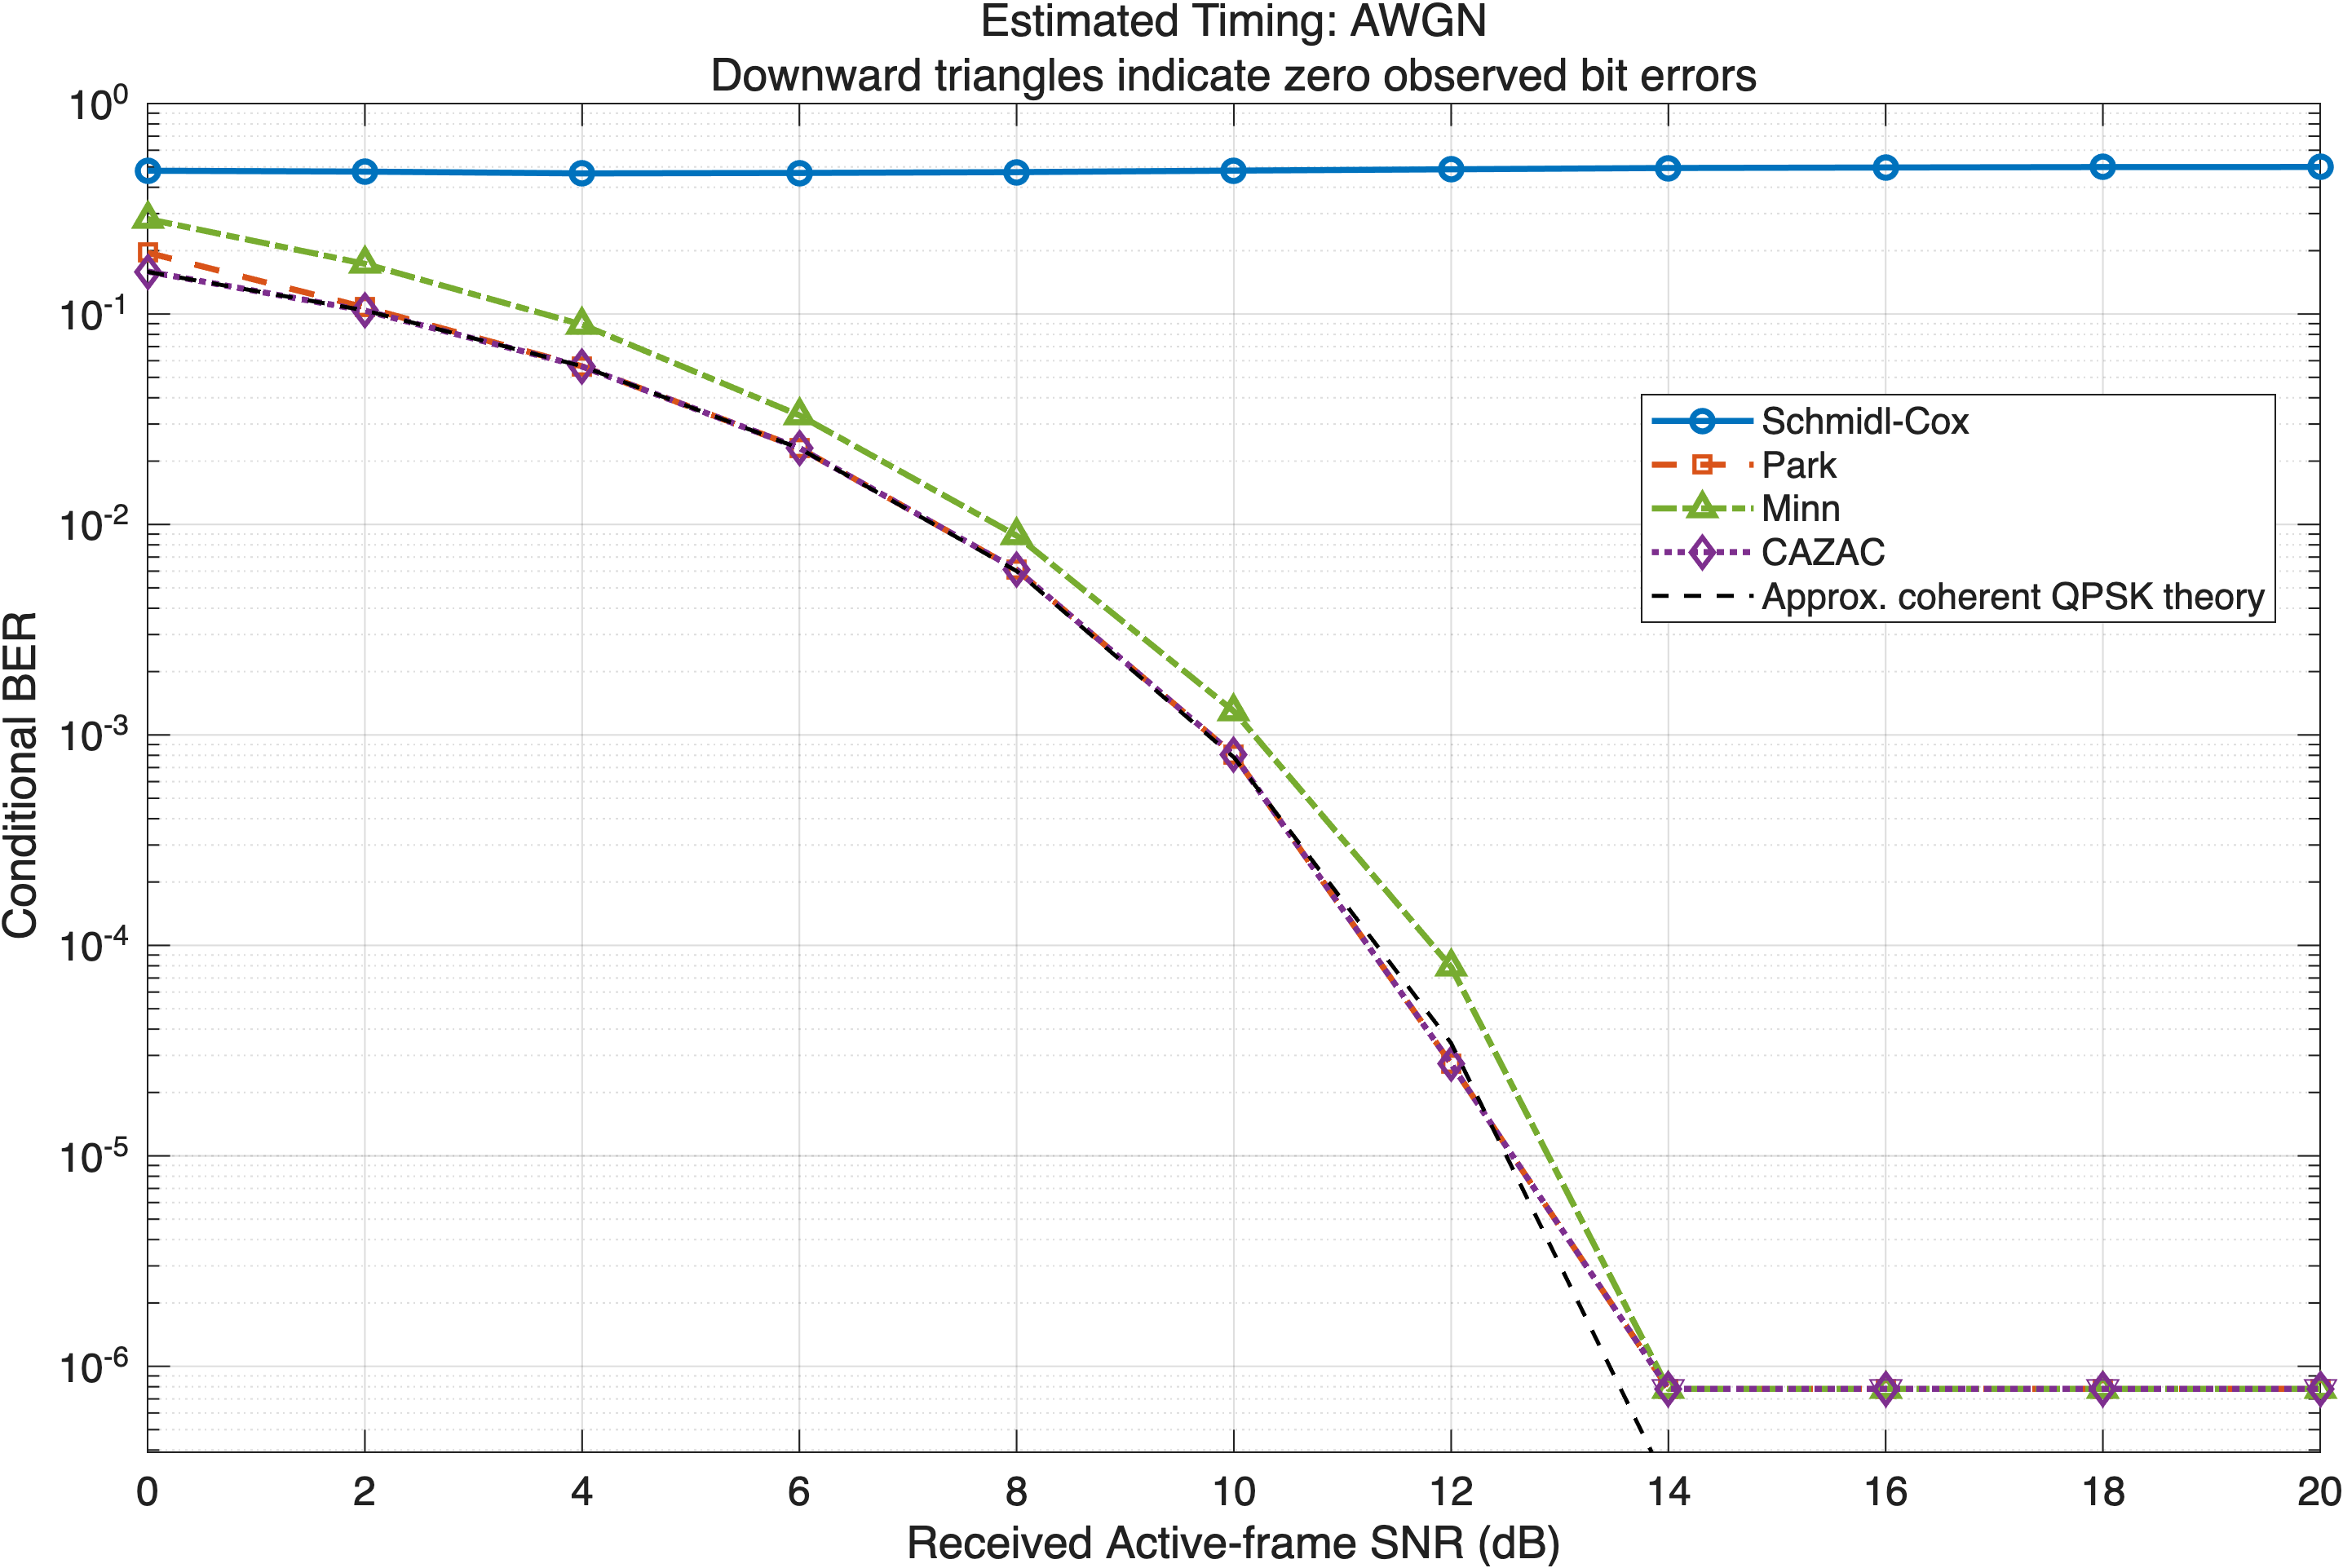
\includegraphics[width=0.90\textwidth,height=0.30\textheight,keepaspectratio]{figures/ch5/exp08_awgn_ber_estimated.png}\par
{\small (a) AWGN}\par\medskip
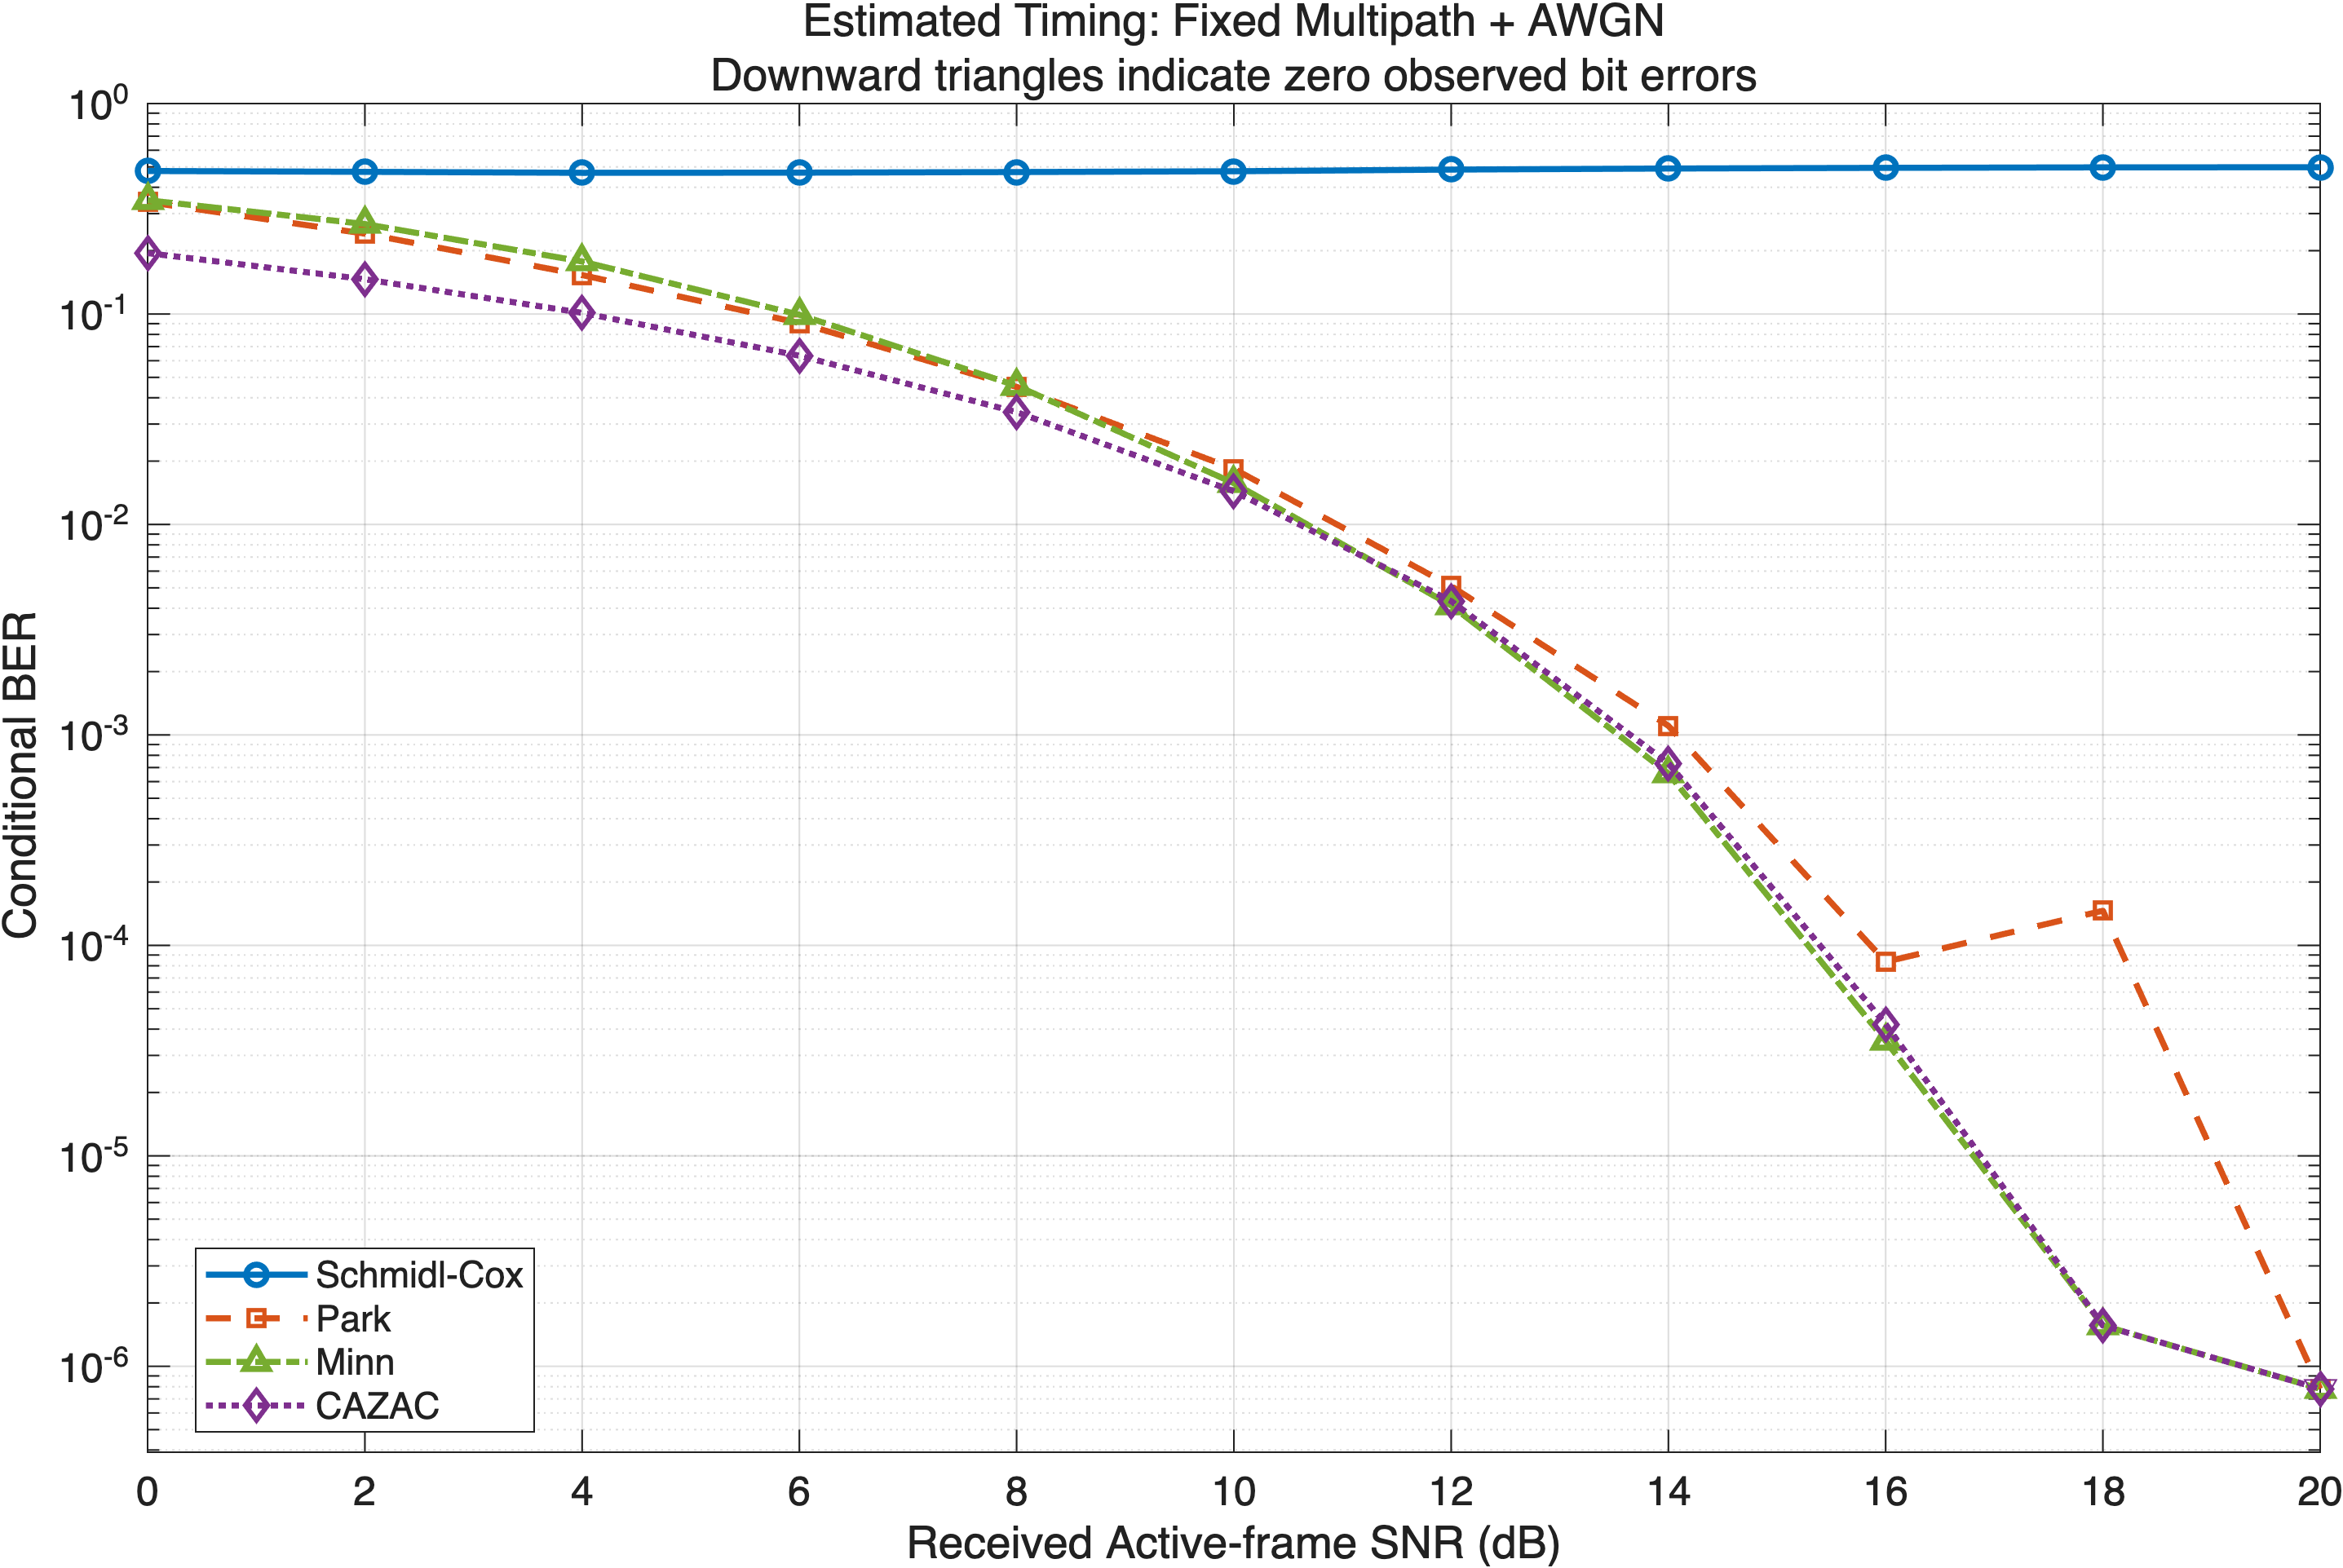
\includegraphics[width=0.90\textwidth,height=0.30\textheight,keepaspectratio]{figures/ch5/exp08_multipath_ber_estimated.png}\par
{\small (b) Fixed multipath with AWGN}
\caption[EXP08: estimated-timing BER.]{EXP08: BER with estimated timing and physical-channel equalization only.}
\label{fig:ch5estimated}
\end{figure}

\begin{table}[!htbp]
\centering\small
\caption[EXP08: bit-error counts in AWGN.]{EXP08: bit-error counts in AWGN. Each entry is based on 1,280,000 decoded bits.}
\label{tab:ch5awgn}
\begin{tabular}{rlrrr}\hline
SNR (dB)&Method&Perfect&Estimated&Oracle\\\hline
0&S\&C&203729&613859&215217\\
 &Park&203729&250434&219592\\
 &Minn&203729&361958&221866\\
 &CAZAC&203729&203729&203729\\\hline
10&S\&C&1029&614662&1296\\
 &Park&1029&1029&1029\\
 &Minn&1029&1657&1199\\
 &CAZAC&1029&1029&1029\\\hline
20&S\&C&0&639428&1\\
 &Park&0&0&0\\
 &Minn&0&0&0\\
 &CAZAC&0&0&0\\\hline
\end{tabular}
\end{table}

\begin{table}[!htbp]
\centering\small
\caption[EXP08: bit-error counts in fixed multipath.]{EXP08: bit-error counts in fixed multipath with AWGN. Each entry is based on 1,280,000 decoded bits.}
\label{tab:ch5mp}
\begin{tabular}{rlrrr}\hline
SNR (dB)&Method&Perfect&Estimated&Oracle\\\hline
0&S\&C&242235&611995&254184\\
 &Park&243741&435782&292434\\
 &Minn&246211&444417&259461\\
 &CAZAC&249122&249240&249121\\\hline
10&S\&C&16293&610322&17375\\
 &Park&16777&23517&16874\\
 &Minn&17511&20102&17548\\
 &CAZAC&18404&18404&18404\\\hline
20&S\&C&0&637574&22\\
 &Park&0&0&0\\
 &Minn&0&0&0\\
 &CAZAC&0&0&0\\\hline
\end{tabular}
\end{table}

\subsection{Performance in AWGN}
At 0 dB, CAZAC returns exact timing for every EXP08 trial and its estimated-timing BER coincides with the perfect reference. Park and Minn have estimated BERs of 0.195652 and 0.282780, respectively. Both exceed the reference of 0.159163 because some windows are displaced. At 10 dB, Park coincides with the reference, while Minn records 1,657 errors compared with the perfect receiver's 1,029. At 20 dB, the three peak-based methods return exact timing and no observed bit errors.

The S\&C result is fundamentally different. Its estimated-timing BER remains close to 0.5 over the SNR grid (0.479577 at 0 dB and 0.499553 at 20 dB). This is not attributable to a failure of the underlying OFDM modulator or FFT: its perfect-timing reference is identical to the other AWGN references. The midpoint decision produces predominantly nonzero early errors, leaving a subcarrier-dependent phase rotation that is not removed by physical-channel equalization.

\subsection{Performance in fixed multipath}
At 0 dB, S\&C has estimated BER 0.478121. The values for Park, Minn and CAZAC are 0.340455, 0.347201 and 0.194719, respectively. Although the Park and Minn curves are close, a comparison of their raw BERs alone conceals the different distributions of timing errors. In EXP08, their CP-safe probabilities at this SNR are 0.5463 and 0.7540, respectively; Minn's larger safe fraction does not imply smaller BER without phase compensation.

By 10 dB the estimated BERs of Park, Minn and CAZAC decrease to 0.018373, 0.015705 and 0.014378, respectively. Their corresponding perfect-timing references are 0.013107, 0.013680 and 0.014378. Thus the remaining synchronization penalties differ even when all three BERs appear similar on a logarithmic plot. At 20 dB all three peak-based designs have no observed bit errors, whereas S\&C has BER 0.498105.

The Park curve in multipath has a small high-SNR irregularity at 18 dB. Examination of its saved frame-level records reveals three nonexact estimates: two errors of $+1$ sample and one of $+10$ samples. These frames contribute 127 and 59 bit errors, respectively, to the uncompensated receiver; one additional error occurs among the 9,997 exactly timed frames. The 187 total errors give BER $1.46094\times10^{-4}$. Oracle compensation reduces the count to one. The subsequent zero-error observation at 20 dB is consistent with rare-event variation; the irregularity is not evidence that increasing SNR systematically worsens the algorithm. These are EXP08 events, distinct from the rare Park errors reported for EXP07.

\section[Oracle Phase Compensation]{Effect of Oracle Phase Compensation}
Figure~\ref{fig:ch5oracle} displays the four algorithms after the oracle compensates the residual phase associated with the true timing error. The compensated receiver still uses the estimated FFT window. It does not move the window back to the correct start. Accordingly, its improvement measures the effect of the supplied phase correction on the existing samples, not a second timing-estimation procedure.

\begin{figure}[!htbp]
\centering
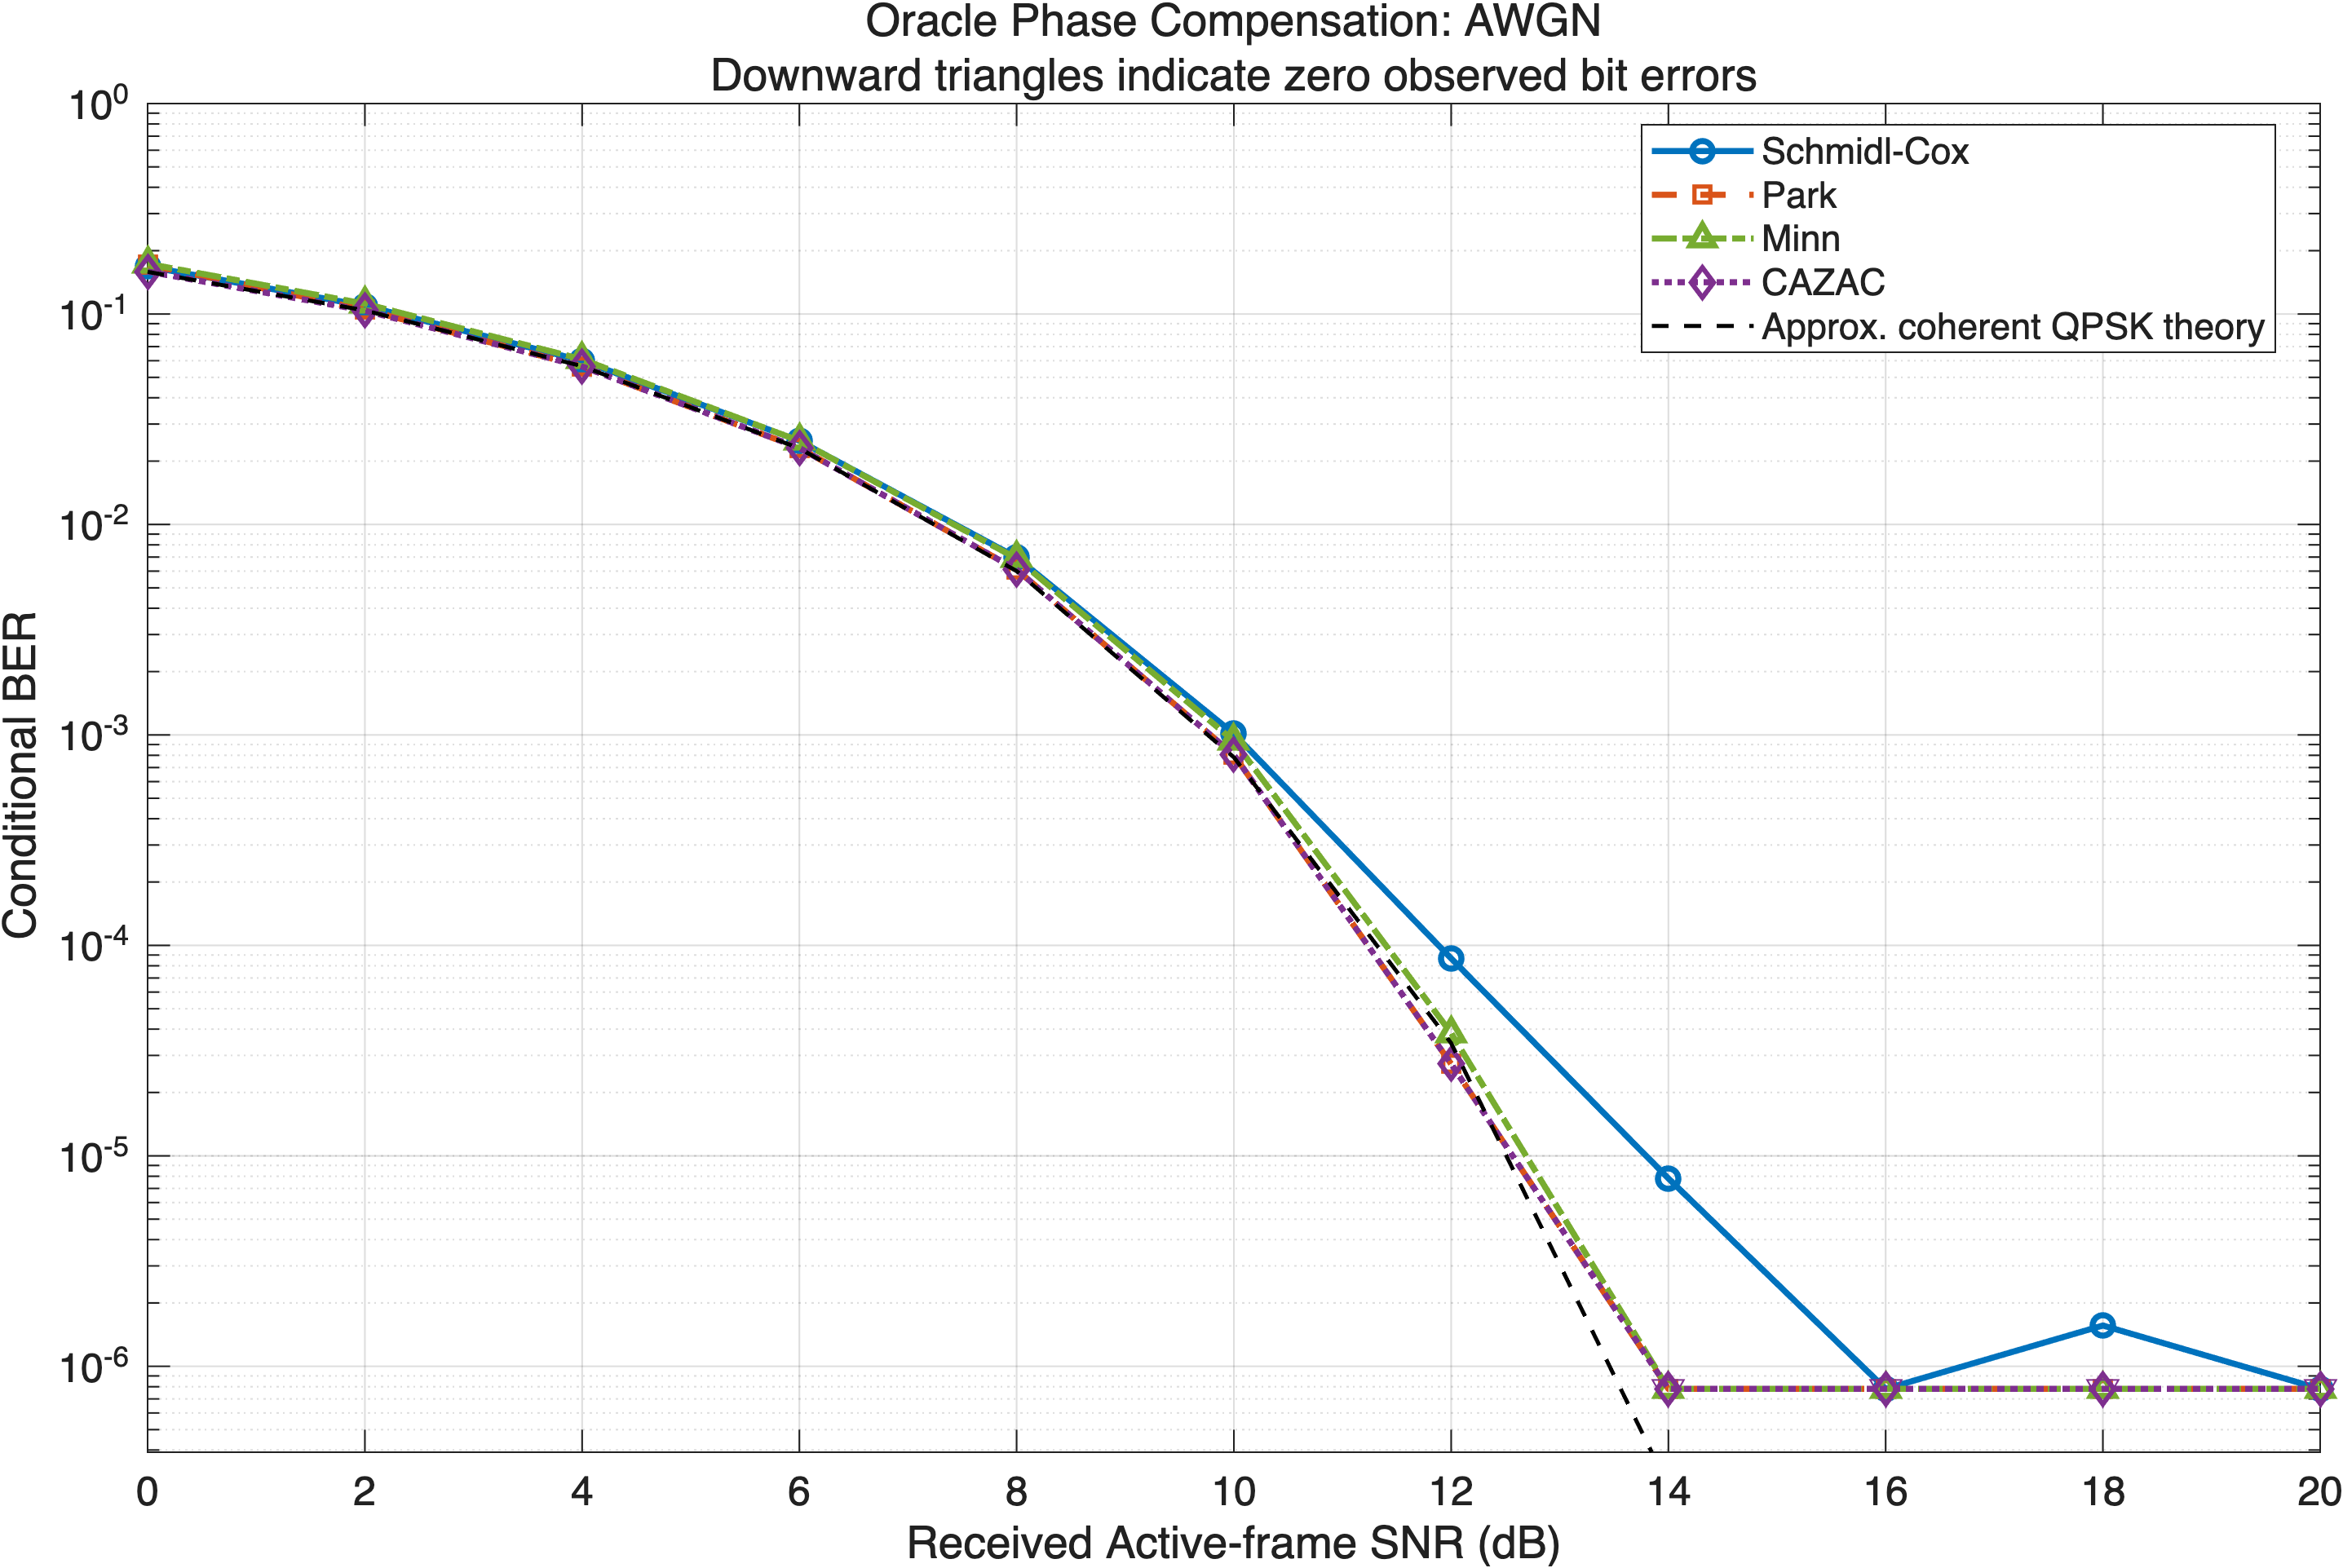
\includegraphics[width=0.90\textwidth,height=0.30\textheight,keepaspectratio]{figures/ch5/exp08_awgn_ber_oracle.png}\par
{\small (a) AWGN}\par\medskip
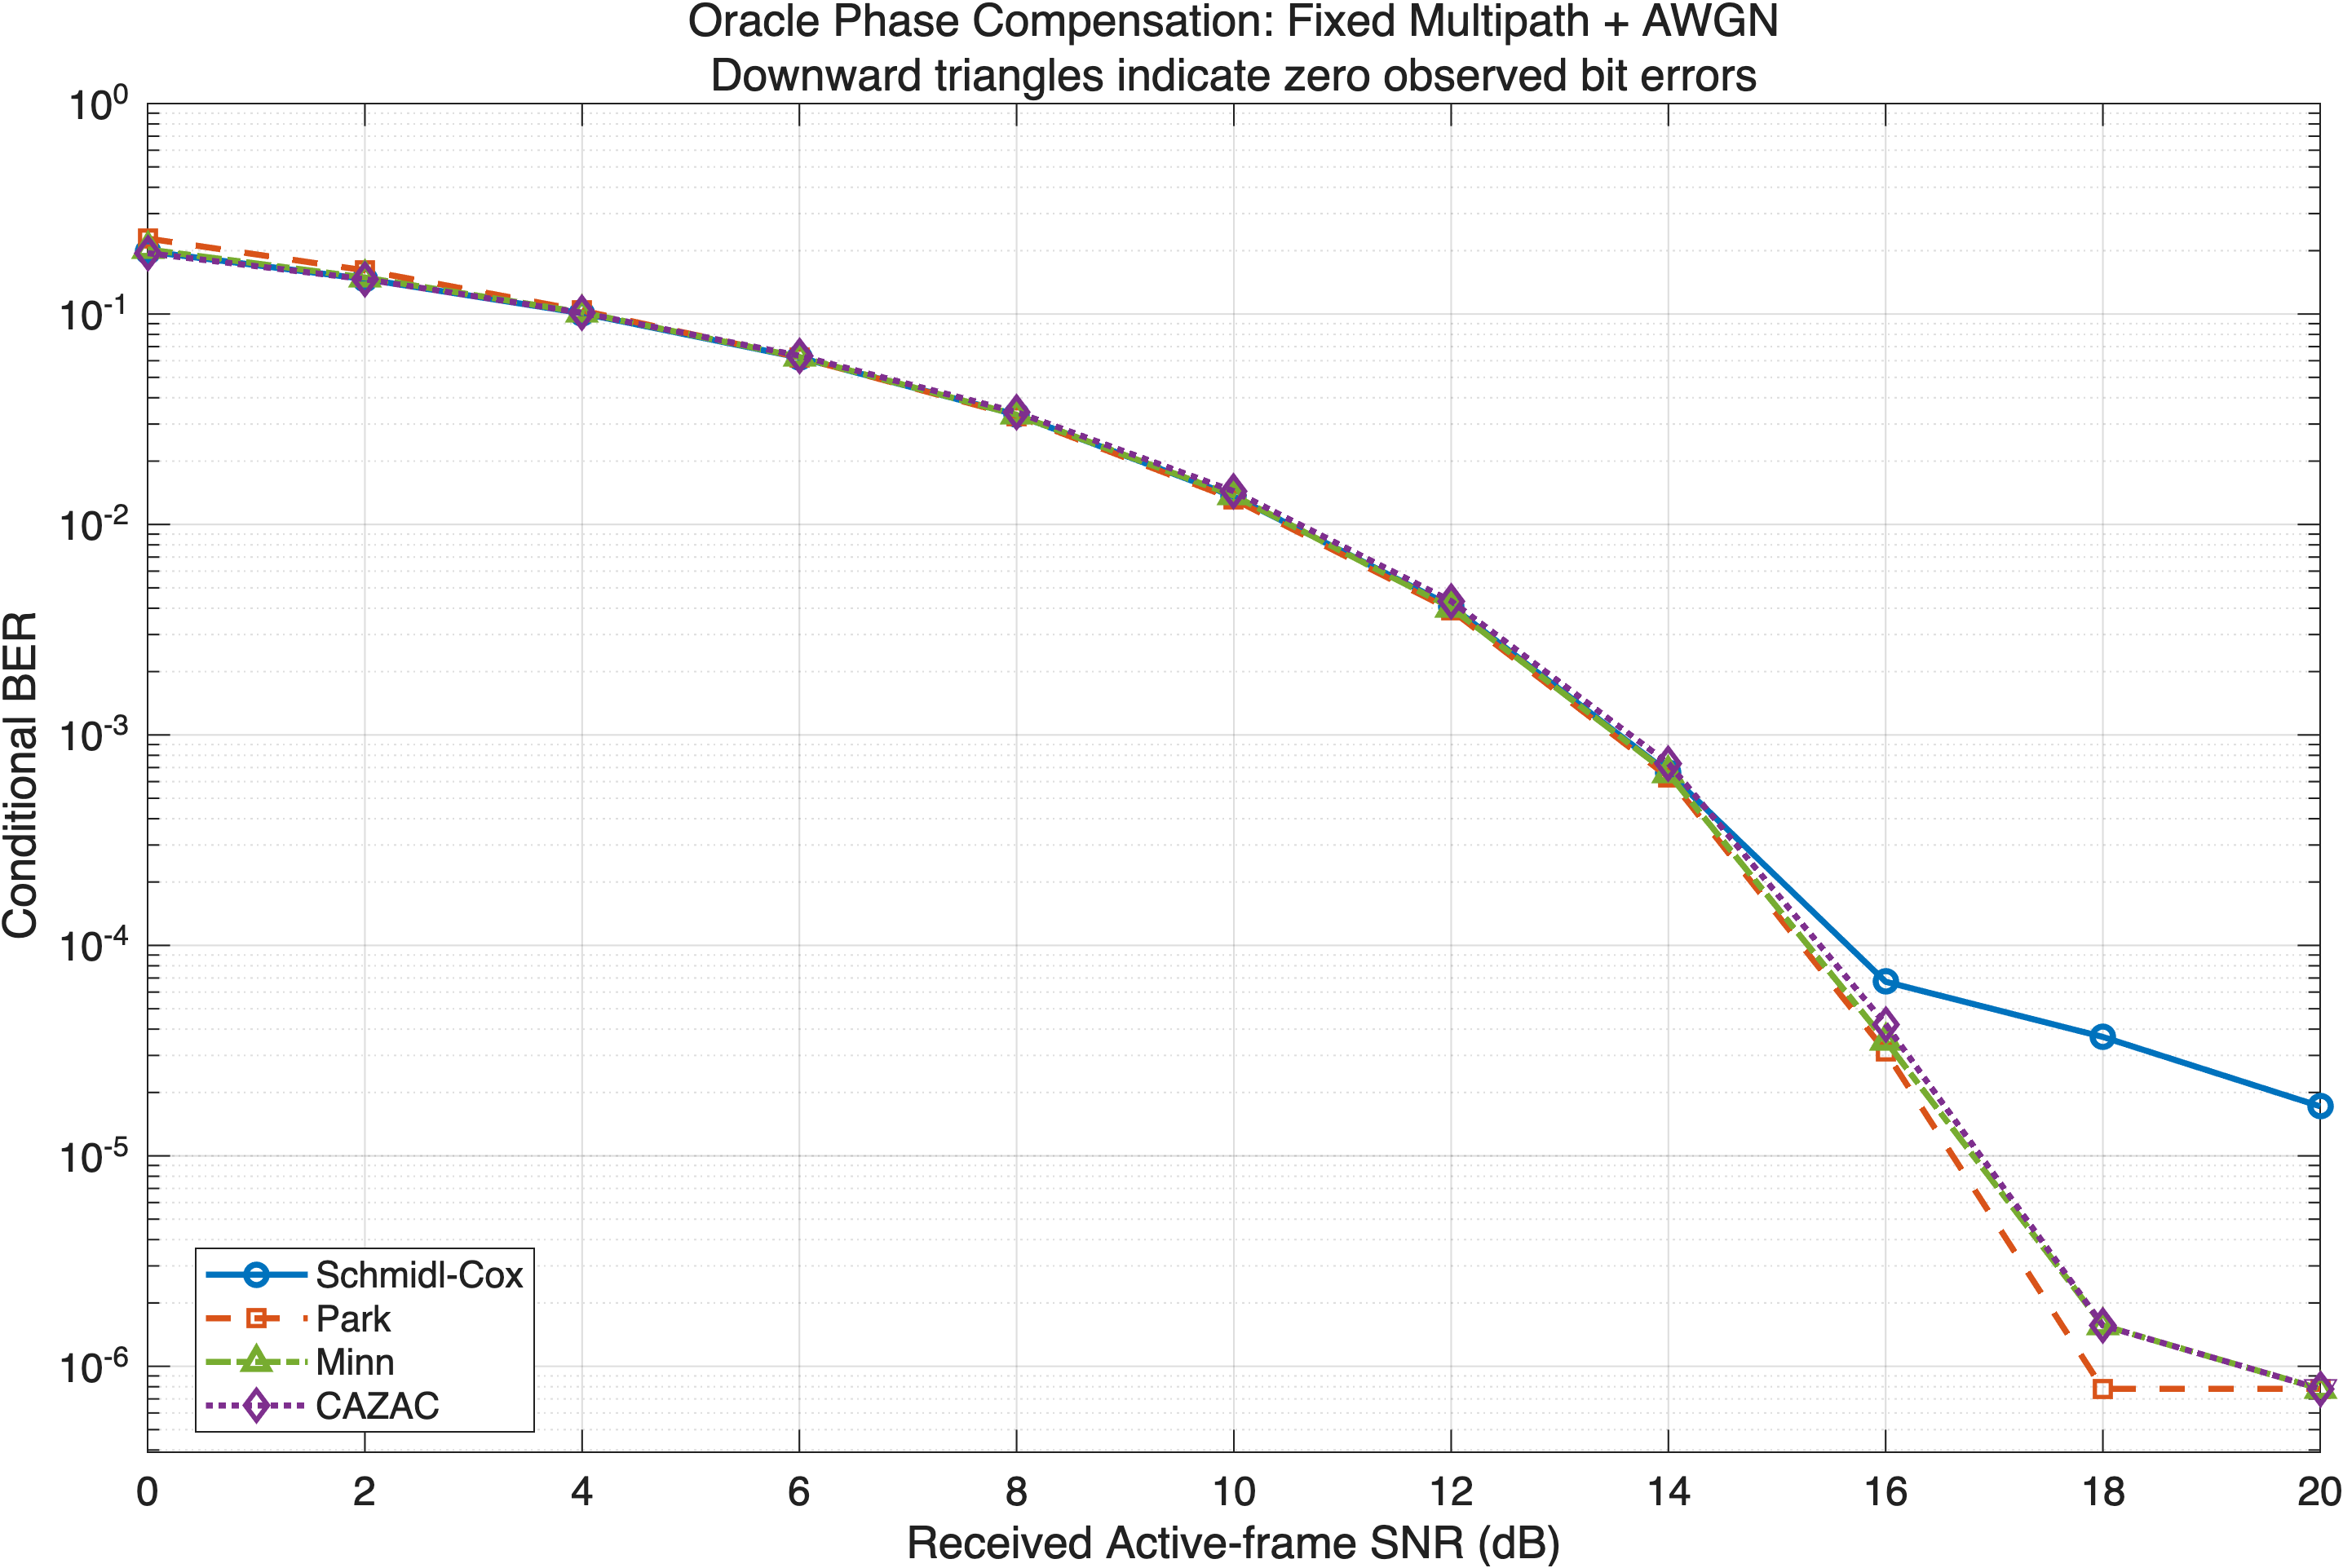
\includegraphics[width=0.90\textwidth,height=0.30\textheight,keepaspectratio]{figures/ch5/exp08_multipath_ber_oracle.png}\par
{\small (b) Fixed multipath with AWGN}
\caption[EXP08: oracle-compensated BER.]{EXP08: BER using the estimated timing window with oracle phase compensation.}
\label{fig:ch5oracle}
\end{figure}

The improvement is most pronounced for S\&C, as illustrated by the direct receiver comparisons in Figure~\ref{fig:ch5sc}. At 10 dB AWGN, its 614,662 uncompensated bit errors decrease to 1,296 with compensation, compared with 1,029 for perfect timing. At 20 dB AWGN, its count decreases from 639,428 to one, while the perfect receiver records zero. In multipath at 20 dB, compensation reduces 637,574 errors to 22. These changes strongly support the phase-rotation mechanism developed in Chapter 2 and verified in EXP02.

\begin{figure}[!htbp]
\centering
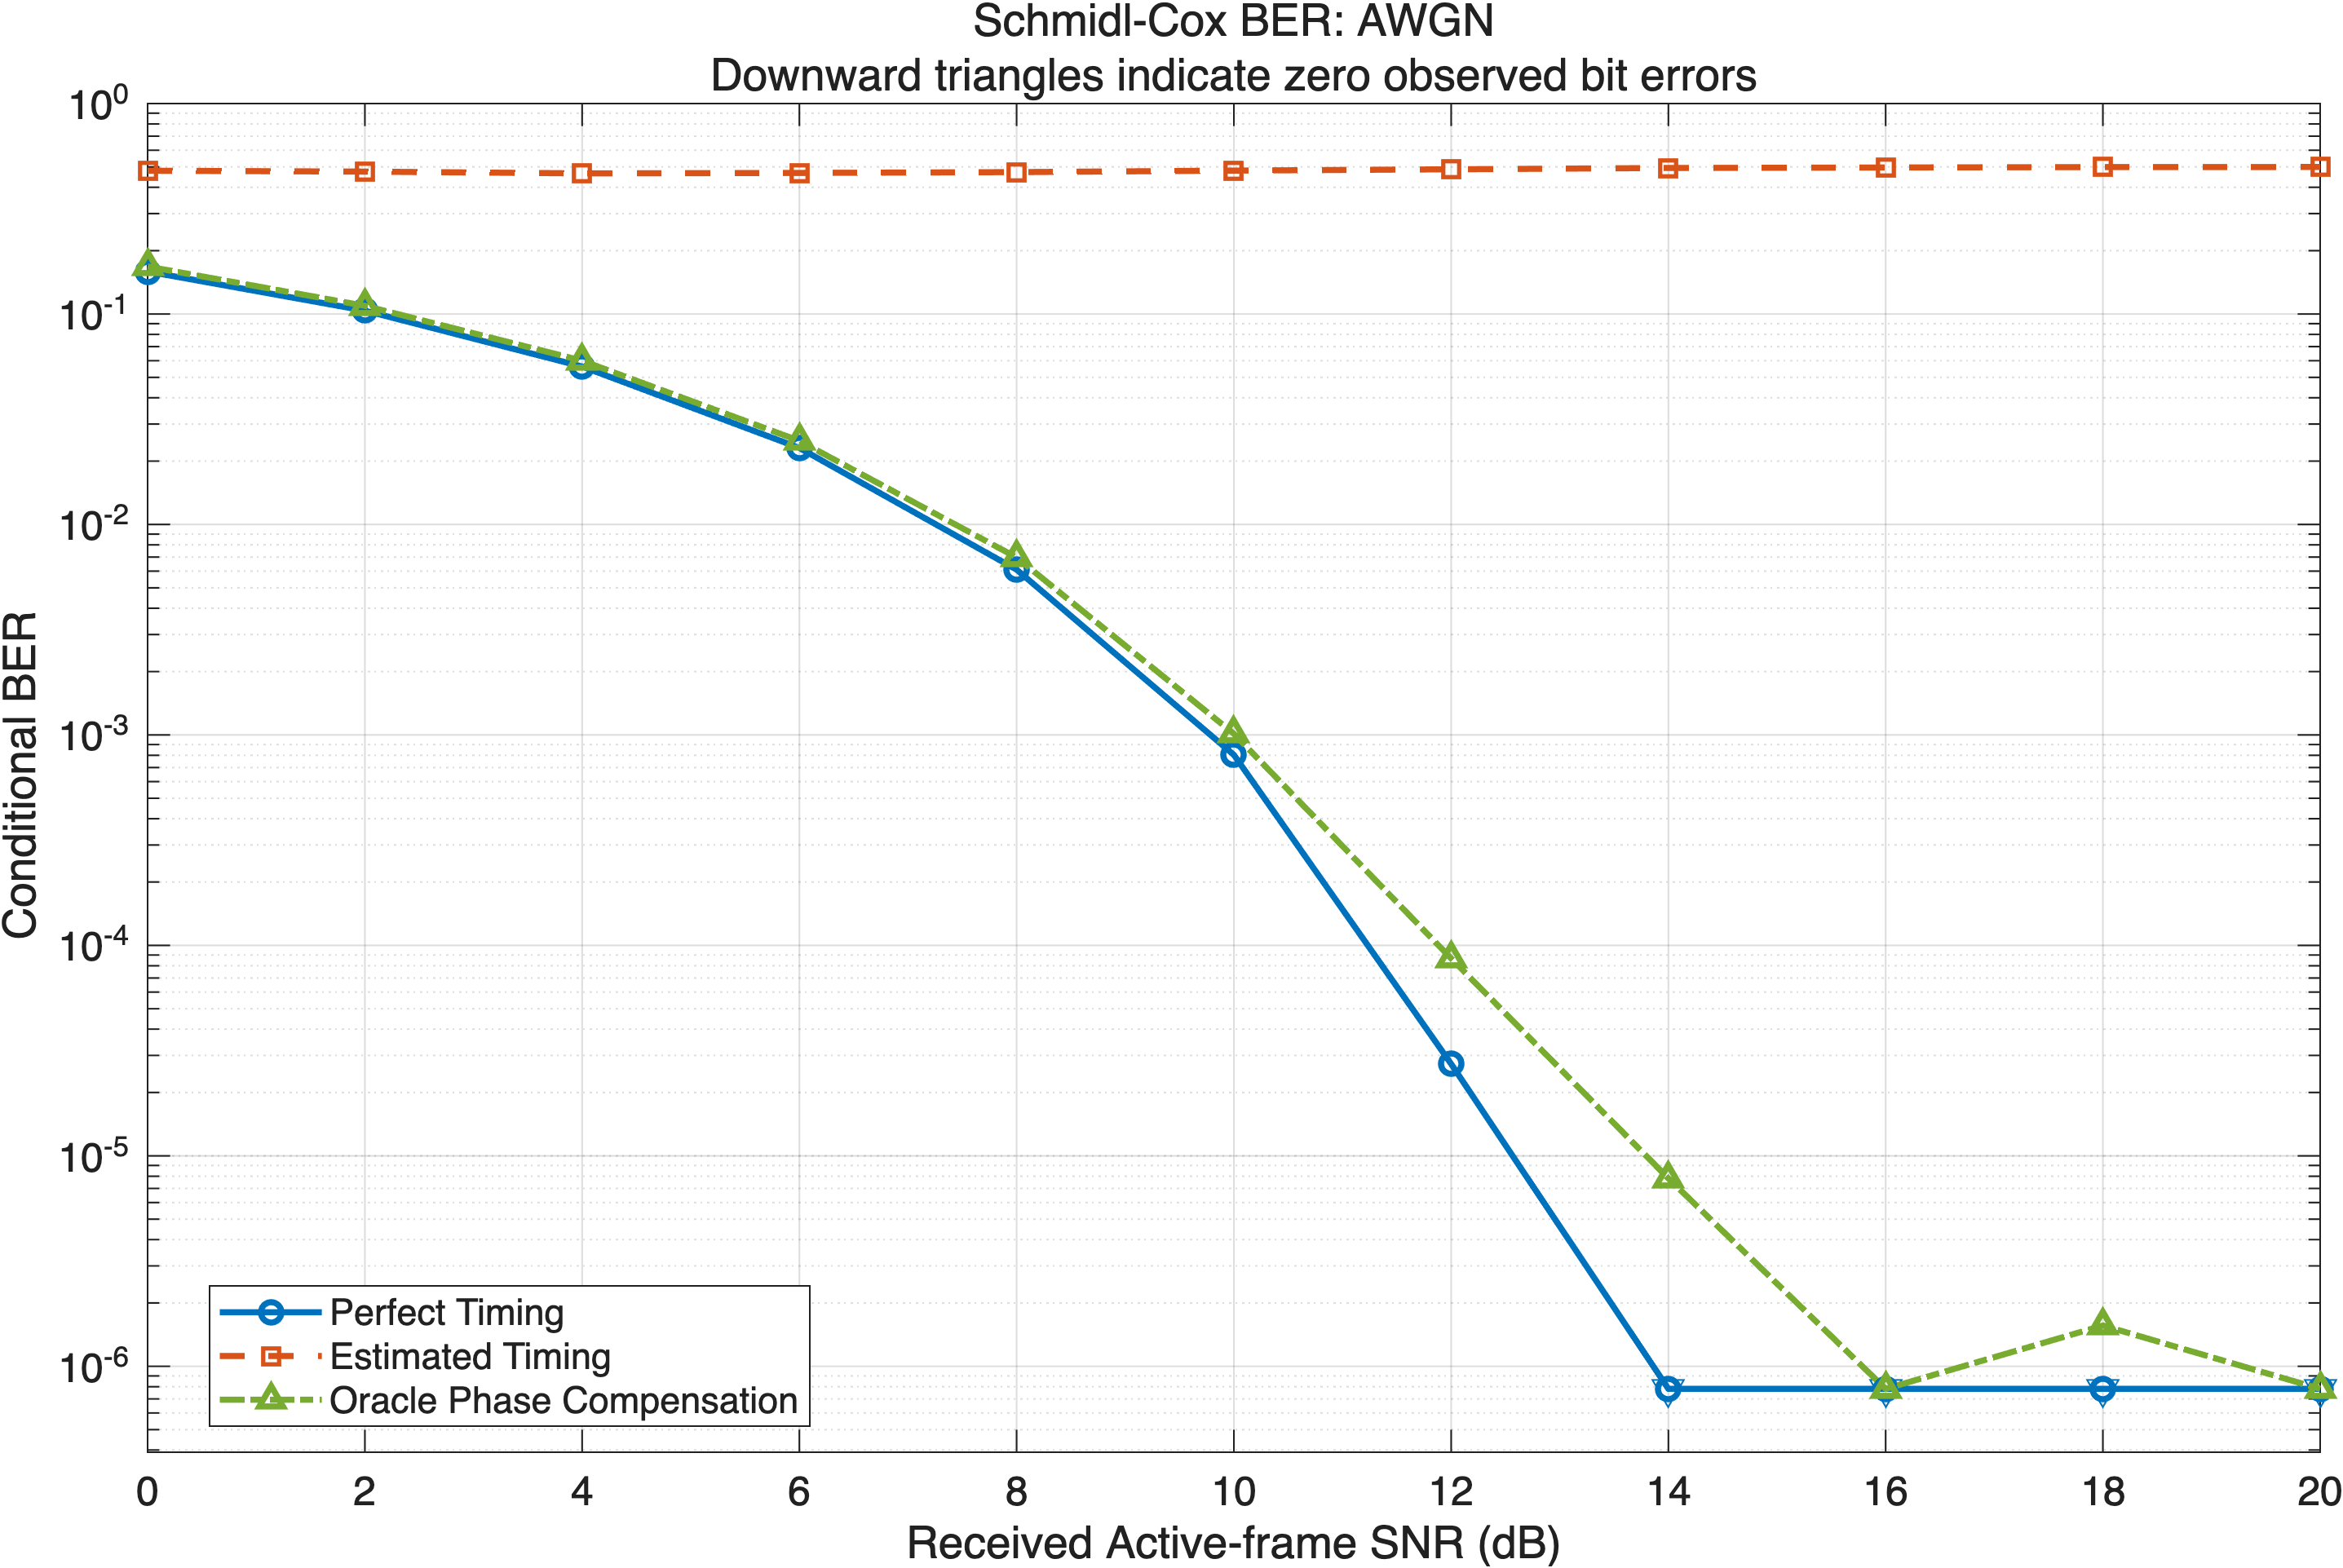
\includegraphics[width=0.90\textwidth,height=0.30\textheight,keepaspectratio]{figures/ch5/exp08_awgn_sc_receiver_comparison.png}\par
{\small (a) AWGN}\par\medskip
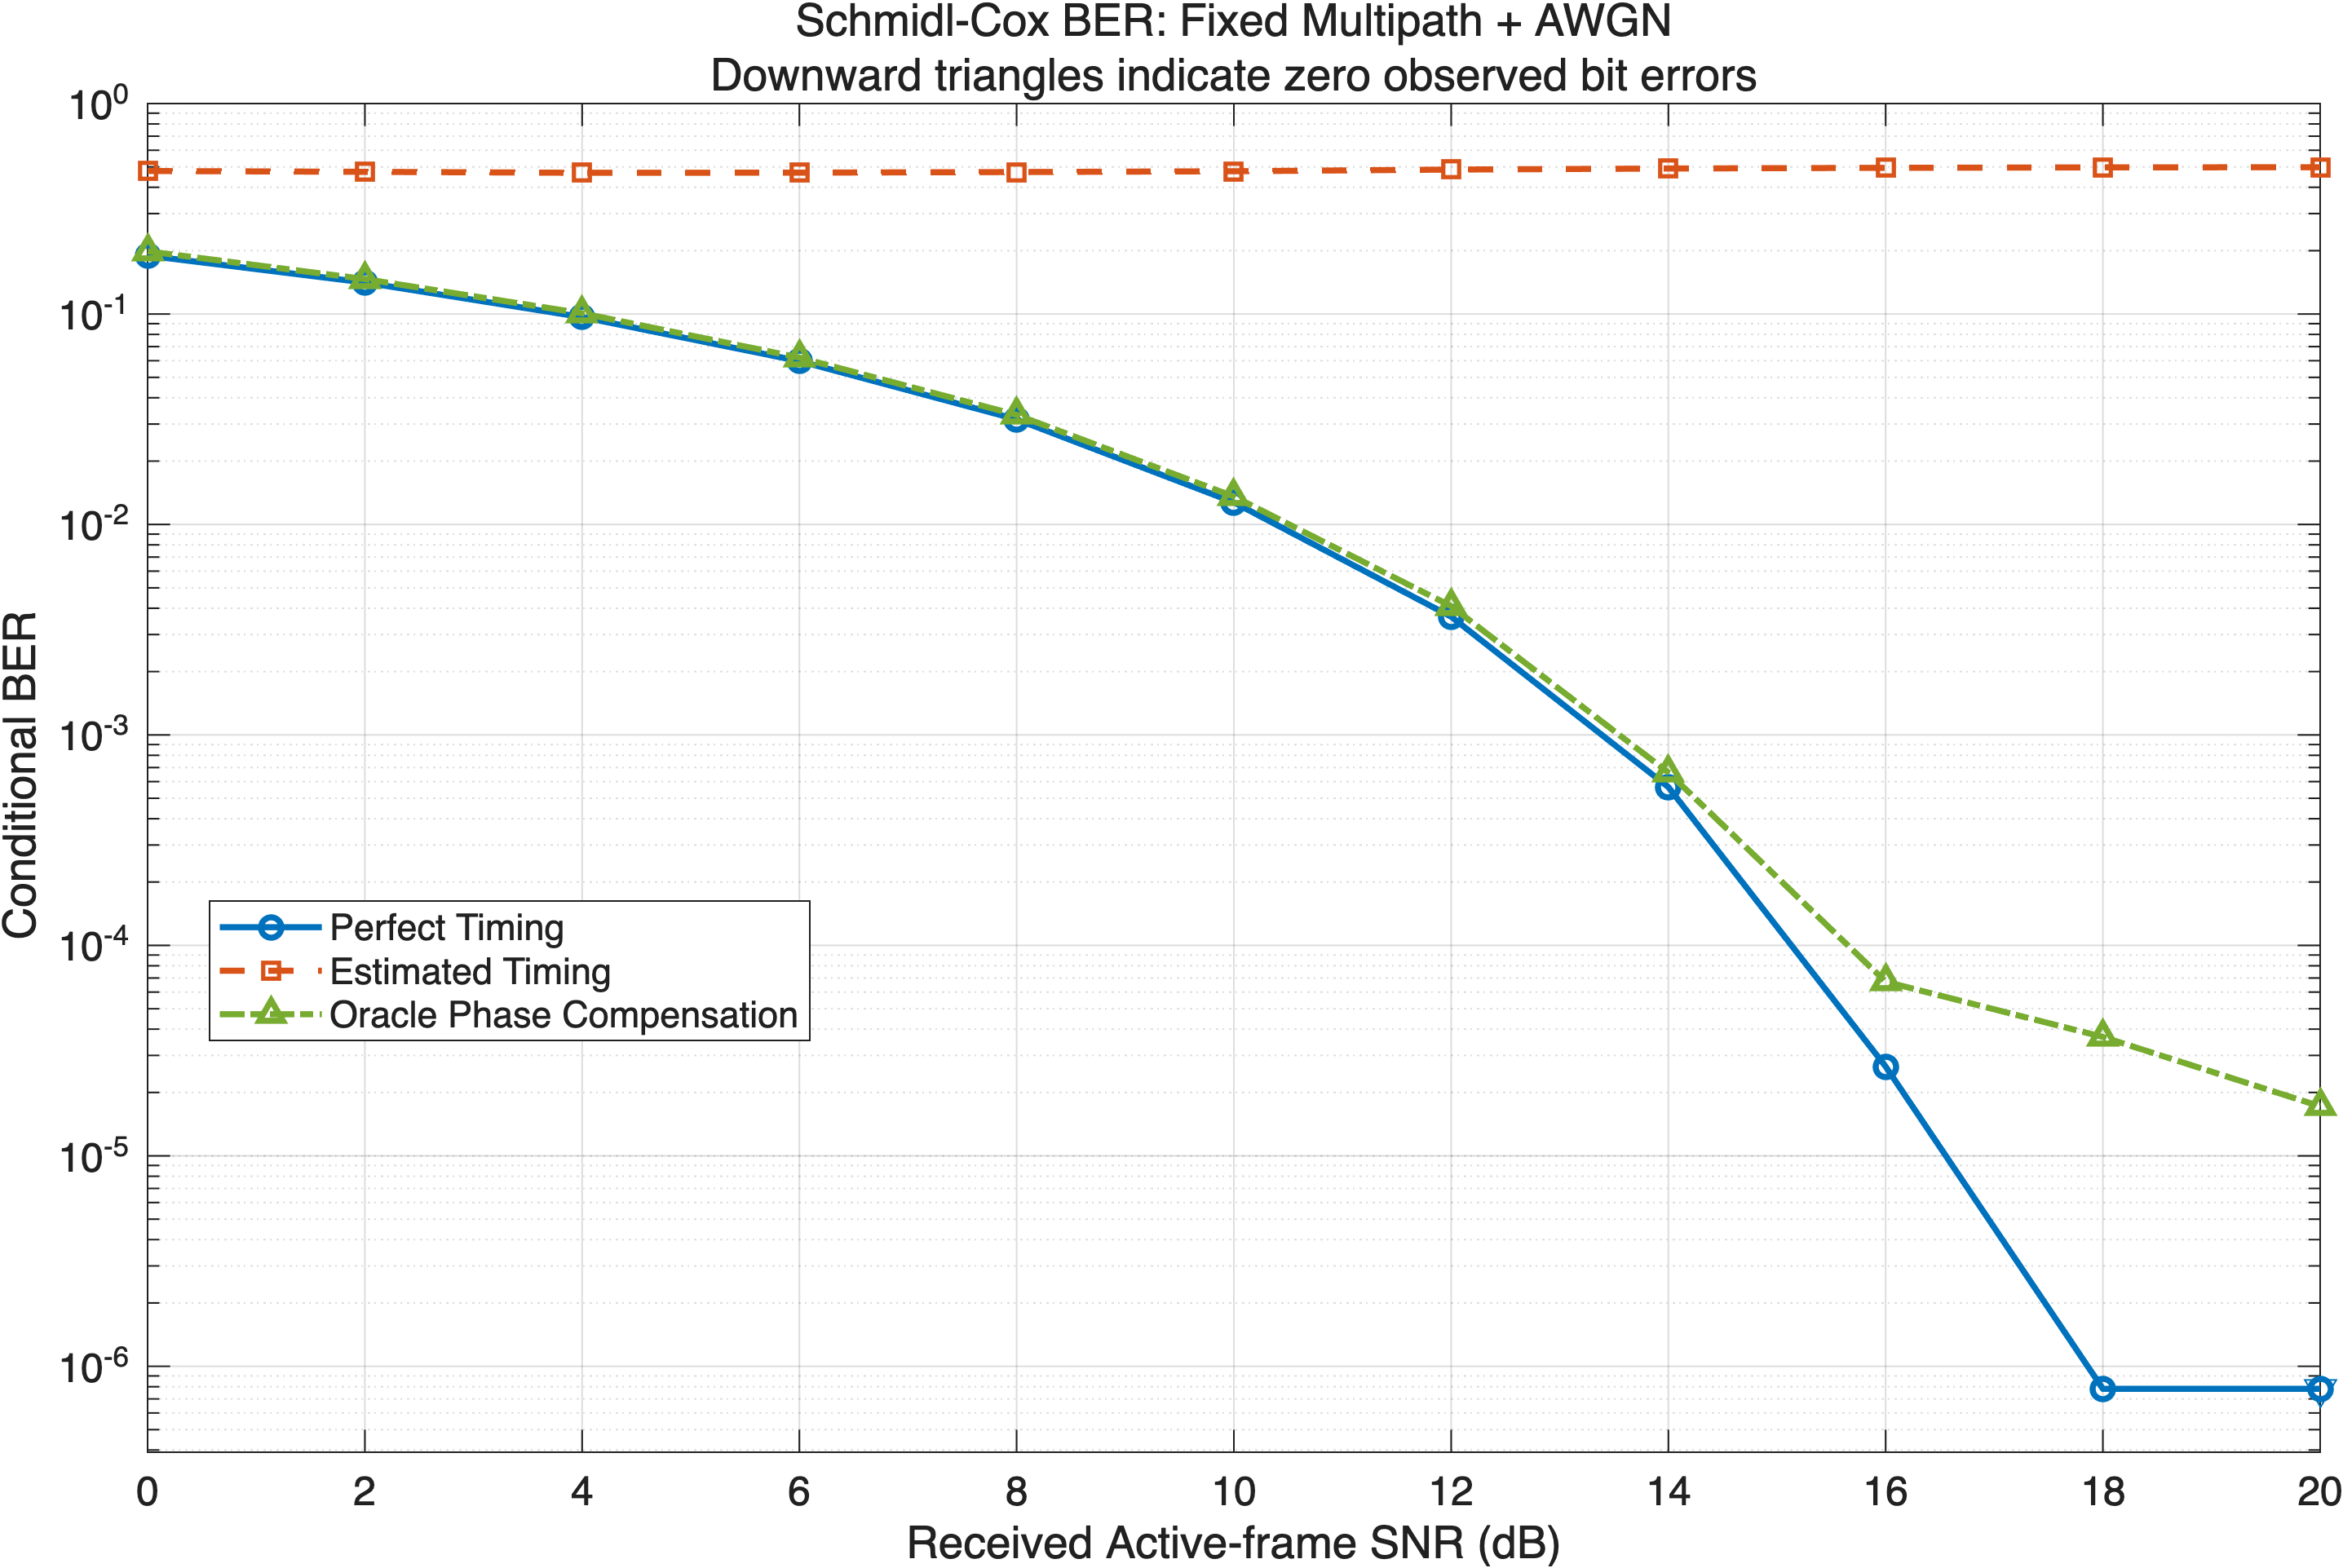
\includegraphics[width=0.90\textwidth,height=0.30\textheight,keepaspectratio]{figures/ch5/exp08_multipath_sc_receiver_comparison.png}\par
{\small (b) Fixed multipath with AWGN}
\caption[EXP08: S\&C receiver comparison.]{EXP08: comparison of perfect, estimated and oracle receiver cases for S\&C.}
\label{fig:ch5sc}
\end{figure}

The peak-based estimators also benefit when nonexact estimates occur. At 0 dB multipath, Park's oracle BER is 0.228464 and Minn's is 0.202704, compared with their respective perfect references of 0.190423 and 0.192352. These differences are consistent with their different error distributions and rates of unsafe-window selection. CAZAC has only three nonexact timing observations across EXP08, all $+1$ sample in 0 dB multipath. For this condition its compensated count (249,121) is one less than the perfect reference (249,122). Small differences of either sign are possible because displaced windows observe different noise samples and can experience different distortion. Perfect timing provides a reference, not a deterministic lower bound on the bit-error count of each realization.

\section[CP-Safe Timing and BER]{Relationship between CP-Safe Timing and BER}
\label{sec:ch5safe}
The aggregate BER can be expressed as a mixture over the estimated-window timing categories. Let $S$ denote a CP-safe timing estimate, and let $U$ be its complement. Since all frames are valid and carry the same number of bits, for a fixed receiver case the empirical decomposition is
\begin{equation}
\widehat{\mathrm{BER}}=\hat p_S\widehat{\mathrm{BER}}_S
 +(1-\hat p_S)\widehat{\mathrm{BER}}_U,
\label{eq:ch5mixture}
\end{equation}
where $\hat p_S$ is the fraction of safe estimates in the same EXP08 condition. A category with no observations has an undefined conditional BER and contributes zero to the total error count. This identity does not require independence between timing error and bit errors.

\begin{table}[!htbp]
\centering\small
\caption[EXP08: S\&C errors by timing category at 20 dB.]{EXP08: S\&C bit-error counts by timing category at 20 dB. Every frame contains 128 decoded bits.}
\label{tab:ch5safe}
\begin{tabular}{llrrr}\hline
Channel&Category&Frames&Estimated&Oracle\\\hline
AWGN&Safe&9981&638209&0\\
&Unsafe&19&1219&1\\\hline
Multipath&Safe&9905&631491&0\\
&Unsafe&95&6083&22\\\hline
\end{tabular}
\end{table}

Table~\ref{tab:ch5safe} shows that 99.81\% of the S\&C estimates in AWGN and 99.05\% in multipath are CP-safe at 20 dB. Nevertheless, the uncompensated BER restricted to safe frames is 0.499550 in AWGN and 0.498084 in multipath. After oracle compensation, there are no observed bit errors among safe frames in either channel. All remaining oracle bit errors occur in the unsafe category. The 19 unsafe AWGN frames produce one error, and the 95 unsafe multipath frames produce 22, giving conditional unsafe BERs of $4.11\times10^{-4}$ and $1.81\times10^{-3}$, respectively. Thus a small fraction of frames accounts for the entire residual error count in these particular high-SNR conditions.

The circular-convolution result in Section~2.3 explains this observation. With physical-channel equalization only and a safe integer offset $e$, the noise-free subcarrier symbol is proportional to
\begin{equation}
X[k]\exp(j2\pi ke/N).
\end{equation}
For the typical nonzero S\&C errors, the phase progression spans the QPSK decision regions. For example, at $e=-7$ the phase sequence visits all 64 equally spaced angles because 7 and 64 are relatively prime. Subcarriers separated by 32 indices then have opposite phase factors. For equiprobable Gray-coded QPSK, decisions related by a rotation of $\pi$ have complementary bit labels; away from decision-boundary ties, the paired bit-error counts average one error per two bits. Symmetric noise also preserves this complementarity in expectation under equal subcarrier noise conditions. This illustrates why the uncompensated aggregate BER can approach 0.5 even when the FFT window is structurally safe. It is not a claim that every nonzero offset, modulation scheme or finite trial must have BER exactly 0.5.

The oracle removes the deterministic phase progression but does not undo ISI, ICI or missing samples outside the safe interval. Conversely, an unsafe estimate need not produce a bit error in every frame, especially for a small displacement at high SNR. Hence exact probability, CP-safe probability and BER should be reported together rather than substituted for one another.

\section[Paired Statistical Interpretation]{Paired Statistical Interpretation}
A comparison of receiver cases on the same frame can quantify the average benefit of oracle compensation without treating the 128 bits within a frame as independent Bernoulli observations. Let $B_{i,E}$ and $B_{i,O}$ be the estimated and oracle bit-error counts for frame $i$, and define the paired frame-level difference
\begin{equation}
\Delta_i=\frac{B_{i,E}-B_{i,O}}{128}.
\end{equation}
Because all frames are valid, the sample mean $\bar\Delta$ equals the difference between the two aggregate BERs. Under independent frame trials within a fixed condition, its estimated Monte Carlo standard error is
\begin{equation}
\widehat{\mathrm{SE}}(\bar\Delta)=
\sqrt{\frac{1}{K(K-1)}\sum_{i=1}^{K}(\Delta_i-\bar\Delta)^2},
\qquad K=10{,}000.
\end{equation}
This estimate accounts for the pairing and allows arbitrary dependence among the bit decisions within each frame. It quantifies simulation uncertainty for the specified condition, not variability across untested channels or hardware.

\begin{table}[!htbp]
\centering\small
\caption[EXP08: paired BER reductions.]{EXP08: mean paired reduction in BER (estimated minus oracle) and its frame-level Monte Carlo standard error.}
\label{tab:ch5paired}
\begin{tabular}{llrr}\hline
Condition&Method&$\bar\Delta$&$\widehat{\mathrm{SE}}$\\\hline
AWGN, 20 dB&S\&C&0.499552&0.000211\\
MP, 20 dB&S\&C&0.498088&0.000270\\
MP, 0 dB&Park&0.111991&0.001287\\
MP, 0 dB&Minn&0.144497&0.001397\\\hline
\end{tabular}
\end{table}

Table~\ref{tab:ch5paired} reports selected conditions calculated directly from the frozen EXP08 bit-error arrays. The high-SNR S\&C reductions of approximately 0.5 are much larger than the corresponding Monte Carlo standard errors. At 0 dB multipath, Minn also shows a substantial reduction despite its slightly higher uncompensated BER than Park. These values describe the benefit of providing the true timing error for phase compensation, not the achievable benefit of an implemented practical phase estimator.

The BER resolution of $1/1{,}280{,}000$ describes the smallest nonzero recorded fraction. It does not by itself quantify statistical uncertainty, because bit errors can cluster within a mistimed frame. In particular, a binomial interval treating all 1,280,000 bits as independent would not be justified by the experimental design. A zero-error condition can instead be interpreted at frame level using the independent-frame assumption, with the same per-condition binomial bound discussed in Section~4.7 for the probability that a frame has any bit error. No simultaneous significance claim over the full grid is made here.

\section[Computational Complexity]{Computational Complexity}
\label{sec:ch5complexity}
A performance comparison is incomplete without considering the processing required to obtain timing estimates. The following analysis counts terms in the direct correlation sums implemented by the frozen MATLAB functions; it is not a measurement of execution time or hardware resource use. Let $C$ denote the number of evaluated candidate positions. For a common decision interval of $C=93$, the repeated-half and mirror correlations each contain $N/2=32$ complex products per candidate. The Minn-type metric computes three adjacent-block correlations of length $N/4=16$, giving 48 products. The CAZAC matched filter uses the entire CP-inclusive preamble and therefore evaluates $N+G=80$ products.

\begin{table}[!htbp]
\centering\small
\caption[Direct correlation workload.]{Direct correlation-product counts. The full-buffer counts describe the metric loops in the frozen implementation; the common-range counts are hypothetical direct evaluations on the 93 decision candidates only.}
\label{tab:ch5complexity}
\begin{tabular}{lrrrr}\hline
Method&Per cand.&93 cand.&Full cand.&Full products\\\hline
S\&C&32&2976&243&7776\\
Park&32&2976&243&7776\\
Minn&48&4464&243&11664\\
CAZAC&80&7440&227&18160\\\hline
\end{tabular}
\end{table}

The actual code computes the metric over every complete window of the 306-sample buffer before restricting its decision range. A 64-sample window therefore yields $306-64+1=243$ candidates, whereas an 80-sample window yields $306-80+1=227$. The resulting direct product counts are shown in Table~\ref{tab:ch5complexity}. The common-range column provides a consistent measure of the principal correlation workload but is not the number of products executed by the frozen code.

The counts exclude the energy calculations, normalization, candidate filtering and decisions. In the full-buffer loops, S\&C calculates 32 received-sample magnitude-squared terms per candidate for the right-half energy. Park calculates 32 such terms for its diagnostic right-half energy, performs a global maximum and normalization, and separately recomputes both half energies (64 terms per candidate) for all 93 positions in the search interval. Minn calculates 64 received-sample energy terms per candidate, and CAZAC calculates 80, plus the 80 template energy terms once per metric call. These correspond to 7,776, 7,776 plus 5,952, 15,552 and 18,160 plus 80 energy terms, respectively. S\&C additionally searches the contiguous threshold region around the selected maximum, while the other estimators select a peak among eligible candidates. Minn's sign weighting and CAZAC's deterministic template generation introduce further operations not included in the complex-product counts.

For direct window-by-window evaluation, the leading correlation complexity is $O(CN)$ for S\&C, Park and Minn, and $O(C(N+G))$ for CAZAC. With a fixed ratio $G/N$, all have the same asymptotic order, but their constant factors and memory requirements differ. A streaming implementation could update certain moving correlation and energy sums recursively; a known-template correlation could also be evaluated by convolution or FFT-based methods. Such optimizations are not implemented or benchmarked in this study. The direct counts do not establish a universal ordering of latency, energy consumption or hardware area.

\section[Overall Discussion]{Overall Discussion and Limitations}
\subsection{Interpretation of the four designs}
The evidence from EXP07 and EXP08 distinguishes three design trade-offs. S\&C uses a comparatively short direct correlation and provides a large safe-window fraction at high SNR, but its particular plateau-midpoint rule does not target the exact useful start. Its poor uncompensated BER reflects the receiver assumptions as well as the timing bias. A practical design might estimate an effective channel from pilots or compensate the residual phase; the oracle demonstrates the potential of phase correction under ideal information, not a deployable solution.

Park and Minn reduce the plateau ambiguity and achieve high exact probabilities at moderate and high SNR. Their low-SNR performance is sensitive to competing peaks and channel distortion. The Park-type method has a relatively short correlation sum, with additional energy gating and global normalization, whereas Minn uses more correlation terms and has a signed-block structure that can yield competing peaks. Their relative merits depend on the choice of exact probability, MSE, safe-window probability and receiver compensation.

The CAZAC-based design produces the strongest empirical timing performance under the selected model, with estimated BER close to its own perfect reference throughout the grid. It also requires the complete known training waveform and has the longest direct correlation sum among the selected implementations. Equal training energy and overhead do not eliminate this receiver-information advantage. The results characterize a known-template design within a bounded search interval rather than prove superiority of all CAZAC-based synchronization algorithms.

\subsection{Limitations of the comparison}
The evaluation is conditional on a simulated, frame-present, integer-delay OFDM model. Only AWGN and one deterministic three-tap multipath channel are tested. The results cannot establish performance under random fading, longer or time-varying channels, fractional-sample timing, carrier-frequency offset or phase noise. The search interval is known in advance; neither unconstrained acquisition nor noise-only false-alarm behavior is assessed. A zero observed timing-failure rate is therefore not a packet-detection guarantee.

The receiver uses the true physical channel response for zero-forcing equalization, and the oracle additionally uses the true timing error. No channel estimation, practical phase tracking, coding, pilot allocation or hardware implementation is evaluated. The equal-energy CP-inclusive normalization and active-frame SNR convention provide a controlled comparison, but the training structures yield different received powers in multipath. The use of algorithm-specific perfect references reduces the risk of attributing those power differences to timing alone.

Finally, the experiments compare representative implemented training-and-estimator combinations, not strict reproductions of every cited algorithm. The results are finite Monte Carlo observations and are not evidence that a theoretical error probability is zero. The operation counts are approximate direct-processing workloads rather than measured execution times. These restrictions define the scope of the conclusions and identify directions for future investigation.

\section{Chapter Summary}
EXP08 links timing accuracy to BER through the FFT-window position and subsequent receiver processing. S\&C exhibits a large uncompensated BER despite a high safe-window probability; oracle compensation removes nearly all its errors at high SNR. Park and Minn generally approach their perfect-timing references as SNR increases, with occasional rare timing errors affecting BER. CAZAC remains close to its reference under the tested conditions, at the cost of a longer direct correlation and stronger prior waveform knowledge. The combined results support the use of multiple timing statistics together with receiver-level BER rather than relying on a single ranking. Chapter 6 summarizes the answers to the research questions and outlines future work.


% Chapter 6: Conclusion and Future Work
\chapter{Conclusion and Future Work}
\label{chap:conclusion}

\section{Summary of the Study}

This study investigated how representative preamble-based timing
synchronization methods affect timing-estimation accuracy and end-to-end
OFDM detection. A modular MATLAB simulation framework was developed
and verified progressively through eight experiments. Baseline verification
and controlled timing displacements established the behavior of the OFDM
link before the four timing estimators were compared. Individual
estimator checks preceded the unified timing experiment (EXP07) and the
end-to-end BER experiment (EXP08).

The formal comparison used a 64-subcarrier QPSK--OFDM system with a
16-sample cyclic prefix, equal CP-inclusive training duration and energy,
and a common useful-symbol timing reference and decision interval.
Each unified experiment contained 10,000 trials for each combination of
four methods, two channel conditions and eleven SNR levels, giving
880,000 timing-estimation attempts per experiment. EXP08 additionally
evaluated three receiver configurations, giving 2,640,000 receiver
observations. The shared trial scenarios supported controlled comparisons,
while EXP07 and EXP08 used distinct random seeds. Timing MSE and
correct-estimation probabilities were the primary evaluation measures;
BER provided complementary receiver-level evidence.

\section[Research Questions]{Answers to the Research Questions}

\subsection*{RQ1: Effects of timing offset}

The baseline BER agreed closely with the theoretical coherent QPSK
reference in AWGN. The controlled-offset experiments demonstrated that
accurate FFT-window placement is essential, but that the effects of timing
offset depend on the channel and receiver processing. For a causal channel
with maximum delay $\nu$ and cyclic-prefix length $G$, the sufficient
CP-safe interval is $[\nu-G,0]$ under the adopted timing convention.
Within this interval, an integer timing displacement preserves the circular
convolution structure but produces a subcarrier-dependent phase rotation.
Outside the interval, interference or loss of the intended samples may
remain even after ideal phase correction. For example, EXP02 showed that
a five-sample early displacement was almost perfectly correctable in the
noiseless symbol-domain experiment, whereas a five-sample late displacement
retained nonzero distortion. Thus, CP protection and correct detection
are distinct properties.

\subsection*{RQ2: Comparison of the four estimators}

The unified timing results showed that metric shape, decision rule and
error distribution jointly determine statistical performance. The selected
Schmidl--Cox (S\&C) midpoint rule retained a systematic early bias associated
with the plateau. At 20 dB AWGN, its exact probability was 0.0006,
whereas its CP-safe probability was 0.9978. Its MSE was 59.4513 samples
squared, approximately 97.36\% of which was attributable to squared
bias. Low noise therefore improved safe-window placement without
eliminating the bias relative to the useful-symbol boundary.

The Park-type and Minn-type methods reduced plateau ambiguity and
achieved much higher exact probabilities at moderate and high SNR.
Nevertheless, occasional large errors could dominate their timing MSE.
The CAZAC-based known-template estimator produced the strongest
empirical timing results: all 110,000 AWGN estimates in EXP07 were
exact, and only three of its 110,000 fixed-multipath estimates were
nonexact, each by one sample. This result is conditional on the selected
waveform, prior information and bounded search interval. The comparison
concerns the implemented designs rather than every version of the
published algorithms.

\subsection*{RQ3: Sensitivity to noise and multipath}

The influence of SNR was not uniform across the estimators. In EXP07,
Park and Minn generally became more accurate as SNR increased, whereas
the S\&C midpoint remained systematically early. The specified multipath
profile was particularly challenging for peak-based estimation at low SNR.
At 0 dB in multipath, Park had a higher exact probability than Minn
(0.4856 versus 0.4653), but its MSE was much larger (322.0781 versus
96.4519 samples squared) and its CP-safe probability was lower (0.5363
versus 0.7605). The choice of performance criterion therefore changes the
relative interpretation of these two designs.

These findings describe AWGN and the particular deterministic three-tap
channel used in the study. The optional investigations of carrier-frequency
offset (CFO) and phase noise in the proposal were not undertaken.
Consequently, the answer to RQ3 is restricted to the completed noise
and multipath experiments.

\subsection*{RQ4: Relationship between timing accuracy and BER}

EXP08 demonstrated that the relationship depends critically on the receiver's
treatment of residual timing error. At 20 dB AWGN, S\&C placed 99.81\%
of its estimated windows within the CP-safe interval, yet its uncompensated
BER was approximately 0.499553. Oracle phase compensation reduced the
bit-error count from 639,428 to one out of 1,280,000 decoded bits. In
fixed multipath at the same SNR, the safe-window fraction was 99.05\%,
and the error count fell from 637,574 to 22 after compensation. In both
conditions, all remaining oracle bit errors occurred in CP-unsafe frames.
The paired frame-level analysis supported the substantial reduction without
requiring independent bit decisions within a frame.

Park, Minn and CAZAC generally approached their respective perfect-timing
BER references as SNR increased. Their references in multipath were
slightly different because the received active-frame power determined the
noise scaling separately for each training design. The appropriate
synchronization penalty is therefore interpreted relative to each method's
own reference. The oracle uses the true timing error, and its performance
quantifies the benefit of ideal phase information rather than that of a
practical phase-estimation algorithm.

\section{Contributions and Implications}

The principal contribution is a controlled statistical comparison of four
representative timing-synchronization implementations, supported by a
verified OFDM framework and saved trial records.
The separation of exact timing, CP-safe timing, MSE and estimator
validity provides a more informative evaluation than a single success
criterion. Error distributions and the bias--variance decomposition explain
why persistent small displacements and rare large errors can lead to
different conclusions even when aggregate probabilities appear favorable.
The receiver comparison and paired BER analysis extend these findings to
data detection. Zero observed errors are interpreted as finite-sample
results, rather than as proof of zero underlying error probability.

The study also highlights a trade-off between timing performance,
receiver-side information and processing cost. Direct correlation at a
single candidate requires 32 complex products for S\&C and Park, 48
for Minn, and 80 for CAZAC under the implemented parameter settings.
These counts describe core correlation workload rather than measured
latency. CAZAC's favorable accuracy is accompanied by a longer correlation
and use of the complete known template; S\&C's shorter correlation and
high safe-window fraction may be useful when effective channel estimation
or residual phase tracking is available. Park and Minn offer alternative
peak-based designs whose relative merits depend on the channel and the
chosen evaluation measure. No universally optimal estimator follows from
this comparison.

\section{Limitations and Future Work}

The conclusions are restricted to integer-sample acquisition in a
frame-present, simulated baseband link with known channel responses,
a single fixed multipath profile, and a bounded search interval. No
practical channel estimator, fractional timing recovery, noise-only
packet detection or hardware implementation was evaluated. The Park-type,
Minn-type and CAZAC-based implementations are representative variants,
not strict reproductions of every cited publication. Equal training
overhead does not ensure identical receiver-side information. These
limitations motivate the following directions for future research.

\begin{enumerate}
\item \textbf{Broader channel and impairment models.}
Extend the comparison to random fading channels, varying path strengths
and delay spreads, fractional-sample delays, CFO and phase noise.
Investigate both timing acquisition and subsequent tracking, including
situations in which the CP is insufficient for the channel delay spread.

\item \textbf{Practical receiver compensation.}
Replace oracle information with pilot-assisted or training-based effective
channel estimation and residual phase correction. Compare the resulting
BER with the existing perfect and oracle references. Investigate whether
plateau-edge refinement or a calibrated midpoint correction can improve
S\&C without sacrificing its safe-window probability; validate any
calibration on independent scenarios.

\item \textbf{Acquisition and information fairness.}
Include wider search intervals, noise-only frames and explicit packet
detection thresholds to quantify missed detections and false alarms.
Compare estimators given the same knowledge of the training waveform,
and examine alternative training lengths and sequence designs.

\item \textbf{Statistics and complexity.}
Use frame-level paired confidence intervals and additional independent
trials to characterize rare errors and uncertainty across channel
realizations. Evaluate recursive correlation updates and FFT-based
matched filtering, with measured execution time and memory use on a
specified platform. Such experiments would complement the approximate
operation counts reported in this thesis.
\end{enumerate}

These proposals have not been implemented.

\section{Concluding Remarks}

The central conclusion is that exact boundary acquisition, structurally
safe FFT-window placement and reliable bit detection are related but
distinct objectives. Under the tested conditions, the selected CAZAC
design achieves the strongest timing accuracy, while the S\&C results
show the importance of residual phase compensation. Timing statistics and
BER should therefore be evaluated together, under explicit assumptions
about the channel, prior information and receiver complexity.


% Appendices
% Replacement for the template's chap-appendix.tex.
% No additional packages required.
\appendix
\chapter[Implementation and Reproducibility]{Implementation and Reproducibility}
\label{app:reproducibility}

This appendix identifies the source files and saved outputs supporting the
experiments in Chapters 3--5. The frozen project archive is the reference
version for this thesis. Supplementary numerical tables in Appendices B and C
are extracted from its saved results, not from new simulation runs.

\section{Project organization}
The MATLAB project is organized into separate configuration, signal processing,
synchronization, experiment and result directories. The principal files and
directories are listed below. Paths are relative to the extracted project root.

\begin{center}
\begin{small}
\begin{tabular}{ll}
\hline
Location & Purpose \\
\hline
\texttt{main.m} & Project initialization \\
\texttt{config/} & Parameters and path management \\
\texttt{src/ofdm/} & Modulation and receiver processing \\
\texttt{src/channel/} & Delay, channel and noise functions \\
\texttt{src/synchronization/} & Training, metrics and decisions \\
\texttt{experiments/} & Validation and Monte Carlo scripts \\
\texttt{results/data/} & MAT files and trial records \\
\texttt{results/tables/} & CSV statistical summaries \\
\texttt{results/figures/} & Original experiment plots \\
\hline
\end{tabular}
\end{small}
\end{center}

The common configuration is defined in \verb|config/default_config.m| and
project paths are managed by \verb|config/project_paths.m|. The initialization
script \verb|main.m| adds the project directories to the MATLAB path; it is
not a command to execute every experiment. The principal synchronization
interface is \verb|timing_estimator_unified.m|, located in the synchronization
source directory. It maps raw estimator positions to a common useful-start
coordinate, applies the candidate range and returns validity information.

The final training and metric pairs are:
\begin{itemize}
\item S\&C: \verb|schmidl_cox_training.m| and \verb|schmidl_cox_metric.m|.
\item Park-type: \verb|park_training_original.m|; metric:
\par\noindent\verb|park_metric_paper2003.m|.
\item Minn-type: \verb|minn_training.m| and \verb|minn_metric.m|.
\item CAZAC: \verb|cazac_training.m| and \verb|cazac_metric.m|.
\end{itemize}
The names of the Park files are historical identifiers; the implemented
variant is the one specified in Chapter 3. Older diagnostic scripts retained
in the archive should not be used in place of the final formal comparison.
The function \verb|ofdm_receive_at_start.m| implements data recovery from a
supplied useful-symbol start in EXP08.

\section{Execution and preservation of results}
The project uses MATLAB with the Communications Toolbox (including QAM and
PSK modulation functions). To initialize a working copy, extract the archive,
set the MATLAB current folder to the extracted project root, and execute:
\begin{verbatim}
main
addpath(genpath(pwd));
rehash;
\end{verbatim}
The baseline and controlled-offset checks are contained in EXP01 and EXP02;
EXP03--06 provide the individual estimator checks. For the final unified
comparison, the following entry points are the relevant scripts:
\begin{verbatim}
exp07_timing_metric_comparison
exp07_unified_monte_carlo
exp08_ber_monte_carlo
\end{verbatim}
The last two scripts use seeds 2045 and 2049, respectively, and obtain the
SNR grid and trial count from the common configuration. They generate distinct
Monte Carlo samples. These commands are provided for reproducibility, not as
an instruction to overwrite the archived evidence. Any rerun should use a
separate copy of the project because the scripts write result files. MATLAB
release, toolbox versions and random-number implementation should be recorded
when replicating the simulation. The reported tables use the existing saved
outputs regardless of any later reruns.

The principal result files, relative to the \texttt{results/} directory, are:
\begin{itemize}
\item \verb|data/exp07_unified_monte_carlo.mat|
\item \verb|tables/exp07_unified_monte_carlo.csv|
\item \verb|data/exp08_ber_monte_carlo.mat|
\item \verb|tables/exp08_timing_statistics.csv|
\item \verb|tables/exp08_ber_monte_carlo.csv|
\end{itemize}
The first experiment records 88 timing-summary rows; the second records 88
timing-summary rows and 264 receiver-specific BER rows. The full CSV files
also retain validity and other diagnostic fields not repeated in the printed
supplementary tables.

\section{Trial Arrays and Verification}
In MATLAB, the timing arrays have dimensions $10000\times11\times2\times4$,
ordered as trial, SNR, channel and algorithm. EXP08 receiver arrays append a
fifth dimension of length three. The channel order is AWGN, fixed multipath;
the algorithm order is S\&C, Park, Minn, CAZAC; and the receiver order is
Perfect, Estimated, Oracle. Arrival delays are stored separately with
trial and SNR dimensions. The two experiments must not be paired across
seeds. The saved EXP08 MAT file uses the MATLAB v7.3 format; software that
reads its HDF5 representation directly must account for the reversed dimension
order relative to MATLAB.

The following read-only MATLAB fragment checks S\&C at 20 dB AWGN.
Cast EXP07 indices to double before subtraction, since some are unsigned.
\begin{small}
\begin{verbatim}
A = load( ...
    'results/data/exp07_unified_monte_carlo.mat');
B = load( ...
    'results/data/exp08_ber_monte_carlo.mat');
s = 11; c = 1; a = 1;
ref = double(A.allArrivalDelays(:,s)) + 17;
e = double(A.estimatedStarts(:,s,c,a)) - ref;
assert(isequal(e,double(A.allErrors(:,s,c,a))));
assert(all(A.allValid(:,s,c,a)));
exact = mean(e == 0);
safe  = mean(e >= -16 & e <= 0);
mse   = mean(e.^2);
ref8 = double(B.allArrivalDelays(:,s)) + 17;
e8 = double(B.allEstimatedStarts(:,s,c,a)) - ref8;
assert(isequal(e8, ...
    double(B.allTimingErrors(:,s,c,a))));
assert(all(B.allTimingValid(:,s,c,a)));
assert(all(B.allReceiverValid(:,s,c,a,:),'all'));
counts = squeeze(sum(B.allBitErrors(:,s,c,a,:),1));
ber = counts / (10000*128);
\end{verbatim}
\end{small}
Expected EXP07 values: exact 0.0006, safe 0.9978 and MSE 59.4513.
Expected EXP08 bit-error counts: 0, 639428 and 1. No new trial is generated.

\chapter[Supplementary Timing Results]{Supplementary Timing Results}
\label{app:timing}
The following tables reproduce the principal EXP07 timing statistics over the
complete SNR grid, using the frozen CSV and trial records. Each row represents
10,000 attempted estimates. All estimates are valid in these data, so the
failure probability is zero in every condition and is omitted from the tables.
Exact and Safe are empirical probabilities, MSE is measured in samples squared,
and Mean, SD and Max are in samples. Mean is the signed error, SD uses the
population-form denominator 10,000, and Max is the maximum absolute error.
Probabilities and MSE are displayed to four decimal places; this precision
retains the resolution of these integer-error summaries. SD is rounded to
four decimal places. Zero entries describe the observed trials only.

\begin{table}[!p]
\centering
\caption{EXP07: AWGN, S\&C and Park.}
\label{app:exp07-0-0}
\small
\setlength{\tabcolsep}{3pt}
\renewcommand{\arraystretch}{1.05}
\begin{tabular}{lrrrrrrr}
\hline
Method & dB & Exact & Safe & MSE & Mean & SD & Max \\
\hline
S\&C & 0 & 0.0576 & 0.6773 & 135.9962 & -7.4264 & 8.9914 & 74 \\
 & 2 & 0.0646 & 0.7600 & 115.1771 & -7.7405 & 7.4338 & 43 \\
 & 4 & 0.0675 & 0.8216 & 103.9654 & -7.6272 & 6.7669 & 32 \\
 & 6 & 0.0624 & 0.8655 & 96.0660 & -7.5908 & 6.2005 & 29 \\
 & 8 & 0.0523 & 0.9179 & 87.3762 & -7.5142 & 5.5599 & 23 \\
 & 10 & 0.0385 & 0.9501 & 81.6839 & -7.5717 & 4.9349 & 19 \\
 & 12 & 0.0227 & 0.9715 & 73.8426 & -7.5214 & 4.1559 & 19 \\
 & 14 & 0.0136 & 0.9857 & 67.1128 & -7.5368 & 3.2108 & 18 \\
 & 16 & 0.0049 & 0.9931 & 62.9007 & -7.5721 & 2.3588 & 17 \\
 & 18 & 0.0015 & 0.9965 & 60.3567 & -7.5949 & 1.6353 & 17 \\
 & 20 & 0.0006 & 0.9978 & 59.4513 & -7.6081 & 1.2522 & 15 \\
\hline
Park & 0 & 0.8981 & 0.9132 & 100.1021 & 0.8549 & 9.9685 & 75 \\
 & 2 & 0.9924 & 0.9939 & 6.5686 & 0.0026 & 2.5629 & 58 \\
 & 4 & 0.9996 & 0.9997 & 0.3328 & -0.0112 & 0.5768 & 32 \\
 & 6 & 1.0000 & 1.0000 & 0.0000 & 0.0000 & 0.0000 & 0 \\
 & 8 & 1.0000 & 1.0000 & 0.0000 & 0.0000 & 0.0000 & 0 \\
 & 10 & 1.0000 & 1.0000 & 0.0000 & 0.0000 & 0.0000 & 0 \\
 & 12 & 0.9999 & 1.0000 & 0.0256 & -0.0016 & 0.1600 & 16 \\
 & 14 & 1.0000 & 1.0000 & 0.0000 & 0.0000 & 0.0000 & 0 \\
 & 16 & 1.0000 & 1.0000 & 0.0000 & 0.0000 & 0.0000 & 0 \\
 & 18 & 1.0000 & 1.0000 & 0.0000 & 0.0000 & 0.0000 & 0 \\
 & 20 & 1.0000 & 1.0000 & 0.0000 & 0.0000 & 0.0000 & 0 \\
\hline
\end{tabular}
\end{table}

\begin{table}[!p]
\centering
\caption{EXP07: AWGN, Minn and CAZAC.}
\label{app:exp07-0-1}
\small
\setlength{\tabcolsep}{3pt}
\renewcommand{\arraystretch}{1.05}
\begin{tabular}{lrrrrrrr}
\hline
Method & dB & Exact & Safe & MSE & Mean & SD & Max \\
\hline
Minn & 0 & 0.6438 & 0.7384 & 116.1906 & -3.1572 & 10.3064 & 63 \\
 & 2 & 0.8222 & 0.8655 & 58.2892 & -1.7700 & 7.4267 & 49 \\
 & 4 & 0.9276 & 0.9431 & 29.4977 & -0.9059 & 5.3551 & 34 \\
 & 6 & 0.9773 & 0.9804 & 12.4727 & -0.3853 & 3.5106 & 32 \\
 & 8 & 0.9949 & 0.9953 & 3.9948 & -0.1244 & 1.9948 & 32 \\
 & 10 & 0.9989 & 0.9989 & 0.9218 & -0.0286 & 0.9597 & 32 \\
 & 12 & 0.9998 & 0.9998 & 0.2048 & -0.0064 & 0.4525 & 32 \\
 & 14 & 1.0000 & 1.0000 & 0.0000 & 0.0000 & 0.0000 & 0 \\
 & 16 & 1.0000 & 1.0000 & 0.0000 & 0.0000 & 0.0000 & 0 \\
 & 18 & 1.0000 & 1.0000 & 0.0000 & 0.0000 & 0.0000 & 0 \\
 & 20 & 1.0000 & 1.0000 & 0.0000 & 0.0000 & 0.0000 & 0 \\
\hline
CAZAC & 0 & 1.0000 & 1.0000 & 0.0000 & 0.0000 & 0.0000 & 0 \\
 & 2 & 1.0000 & 1.0000 & 0.0000 & 0.0000 & 0.0000 & 0 \\
 & 4 & 1.0000 & 1.0000 & 0.0000 & 0.0000 & 0.0000 & 0 \\
 & 6 & 1.0000 & 1.0000 & 0.0000 & 0.0000 & 0.0000 & 0 \\
 & 8 & 1.0000 & 1.0000 & 0.0000 & 0.0000 & 0.0000 & 0 \\
 & 10 & 1.0000 & 1.0000 & 0.0000 & 0.0000 & 0.0000 & 0 \\
 & 12 & 1.0000 & 1.0000 & 0.0000 & 0.0000 & 0.0000 & 0 \\
 & 14 & 1.0000 & 1.0000 & 0.0000 & 0.0000 & 0.0000 & 0 \\
 & 16 & 1.0000 & 1.0000 & 0.0000 & 0.0000 & 0.0000 & 0 \\
 & 18 & 1.0000 & 1.0000 & 0.0000 & 0.0000 & 0.0000 & 0 \\
 & 20 & 1.0000 & 1.0000 & 0.0000 & 0.0000 & 0.0000 & 0 \\
\hline
\end{tabular}
\end{table}

\begin{table}[!p]
\centering
\caption{EXP07: Fixed multipath with AWGN, S\&C and Park.}
\label{app:exp07-1-0}
\small
\setlength{\tabcolsep}{3pt}
\renewcommand{\arraystretch}{1.05}
\begin{tabular}{lrrrrrrr}
\hline
Method & dB & Exact & Safe & MSE & Mean & SD & Max \\
\hline
S\&C & 0 & 0.0561 & 0.5611 & 136.6196 & -6.9732 & 9.3805 & 74 \\
 & 2 & 0.0635 & 0.6242 & 113.7913 & -7.3957 & 7.6873 & 63 \\
 & 4 & 0.0641 & 0.6878 & 100.7103 & -7.3505 & 6.8323 & 29 \\
 & 6 & 0.0621 & 0.7445 & 92.1388 & -7.2608 & 6.2785 & 31 \\
 & 8 & 0.0509 & 0.8181 & 83.0025 & -7.1595 & 5.6342 & 27 \\
 & 10 & 0.0393 & 0.8753 & 76.9561 & -7.2113 & 4.9953 & 20 \\
 & 12 & 0.0267 & 0.9215 & 69.7334 & -7.1676 & 4.2847 & 20 \\
 & 14 & 0.0142 & 0.9585 & 63.4962 & -7.2118 & 3.3891 & 18 \\
 & 16 & 0.0074 & 0.9794 & 59.6080 & -7.2730 & 2.5907 & 17 \\
 & 18 & 0.0029 & 0.9875 & 56.5460 & -7.2472 & 2.0060 & 17 \\
 & 20 & 0.0013 & 0.9924 & 55.6819 & -7.2907 & 1.5898 & 16 \\
\hline
Park & 0 & 0.4856 & 0.5363 & 322.0781 & 4.9677 & 17.2453 & 75 \\
 & 2 & 0.7200 & 0.7377 & 130.2631 & 2.4615 & 11.1447 & 76 \\
 & 4 & 0.8466 & 0.8524 & 39.8540 & 0.8804 & 6.2513 & 72 \\
 & 6 & 0.9302 & 0.9316 & 8.7257 & 0.2591 & 2.9425 & 64 \\
 & 8 & 0.9723 & 0.9727 & 1.6678 & 0.0658 & 1.2898 & 50 \\
 & 10 & 0.9902 & 0.9905 & 0.8639 & 0.0289 & 0.9290 & 51 \\
 & 12 & 0.9964 & 0.9964 & 0.1430 & 0.0080 & 0.3781 & 36 \\
 & 14 & 0.9990 & 0.9991 & 0.0178 & -0.0004 & 0.1334 & 13 \\
 & 16 & 0.9998 & 0.9998 & 0.0002 & 0.0002 & 0.0141 & 1 \\
 & 18 & 1.0000 & 1.0000 & 0.0000 & 0.0000 & 0.0000 & 0 \\
 & 20 & 0.9999 & 0.9999 & 0.0361 & 0.0019 & 0.1900 & 19 \\
\hline
\end{tabular}
\end{table}

\begin{table}[!p]
\centering
\caption{EXP07: Fixed multipath with AWGN, Minn and CAZAC.}
\label{app:exp07-1-1}
\small
\setlength{\tabcolsep}{3pt}
\renewcommand{\arraystretch}{1.05}
\begin{tabular}{lrrrrrrr}
\hline
Method & dB & Exact & Safe & MSE & Mean & SD & Max \\
\hline
Minn & 0 & 0.4653 & 0.7605 & 96.4519 & -2.9189 & 9.3772 & 71 \\
 & 2 & 0.6300 & 0.8661 & 42.6963 & -1.5923 & 6.3373 & 37 \\
 & 4 & 0.7864 & 0.9457 & 16.1942 & -0.7040 & 3.9621 & 34 \\
 & 6 & 0.9121 & 0.9821 & 3.8823 & -0.2117 & 1.9589 & 34 \\
 & 8 & 0.9752 & 0.9985 & 0.2696 & -0.0418 & 0.5175 & 32 \\
 & 10 & 0.9955 & 0.9998 & 0.1140 & -0.0098 & 0.3375 & 32 \\
 & 12 & 0.9996 & 1.0000 & 0.0007 & -0.0005 & 0.0265 & 2 \\
 & 14 & 1.0000 & 1.0000 & 0.0000 & 0.0000 & 0.0000 & 0 \\
 & 16 & 1.0000 & 1.0000 & 0.0000 & 0.0000 & 0.0000 & 0 \\
 & 18 & 1.0000 & 1.0000 & 0.0000 & 0.0000 & 0.0000 & 0 \\
 & 20 & 1.0000 & 1.0000 & 0.0000 & 0.0000 & 0.0000 & 0 \\
\hline
CAZAC & 0 & 0.9998 & 0.9998 & 0.0002 & 0.0002 & 0.0141 & 1 \\
 & 2 & 0.9999 & 0.9999 & 0.0001 & 0.0001 & 0.0100 & 1 \\
 & 4 & 1.0000 & 1.0000 & 0.0000 & 0.0000 & 0.0000 & 0 \\
 & 6 & 1.0000 & 1.0000 & 0.0000 & 0.0000 & 0.0000 & 0 \\
 & 8 & 1.0000 & 1.0000 & 0.0000 & 0.0000 & 0.0000 & 0 \\
 & 10 & 1.0000 & 1.0000 & 0.0000 & 0.0000 & 0.0000 & 0 \\
 & 12 & 1.0000 & 1.0000 & 0.0000 & 0.0000 & 0.0000 & 0 \\
 & 14 & 1.0000 & 1.0000 & 0.0000 & 0.0000 & 0.0000 & 0 \\
 & 16 & 1.0000 & 1.0000 & 0.0000 & 0.0000 & 0.0000 & 0 \\
 & 18 & 1.0000 & 1.0000 & 0.0000 & 0.0000 & 0.0000 & 0 \\
 & 20 & 1.0000 & 1.0000 & 0.0000 & 0.0000 & 0.0000 & 0 \\
\hline
\end{tabular}
\end{table}

\clearpage
\chapter[Supplementary BER Results]{Supplementary BER Results}
\label{app:ber}
EXP08 uses its own trial realizations. The timing columns below reproduce
its 88 condition-level timing summaries (not EXP07 summaries). The three
receiver columns report exact bit-error counts for 264 conditions
across the three receiver configurations. Every row has 10,000 frames, with 128 bits decoded per frame
for each receiver. All timing and receiver validity flags are true; there
are no observed lost bits. Hence the BER for any receiver entry is its bit-error
count divided by 1,280,000. Counts are printed rather than rounded BERs to
preserve the distinction between zero errors and one or more rare errors.
Mean is the mean signed timing error, and the MSE unit is samples squared.
The Safe criterion is $[-16,0]$ in AWGN and $[-14,0]$ in fixed multipath.
The complete CSV additionally contains conditional safe and unsafe BER,
frame counts, and delivery-failure statistics. In that file an empty timing
category has an undefined conditional BER (NaN), not an observed BER of zero.

\begin{table}[!p]
\centering
\caption{EXP08: AWGN, S\&C and Park. Receiver columns are bit-error counts.}
\label{app:exp08-0-0}
\small
\setlength{\tabcolsep}{3pt}
\renewcommand{\arraystretch}{1.05}
\begin{tabular}{lrrrrrrrr}
\hline
Method & dB & Exact & Safe & MSE & Mean & Perfect & Est. & Oracle \\
\hline
S\&C & 0 & 0.0596 & 0.6782 & 138.8923 & -7.5843 & 203729 & 613859 & 215217 \\
 & 2 & 0.0630 & 0.7629 & 114.7761 & -7.6691 & 132804 & 607946 & 140054 \\
 & 4 & 0.0769 & 0.8136 & 103.7471 & -7.5979 & 72039 & 596189 & 76822 \\
 & 6 & 0.0666 & 0.8713 & 94.4894 & -7.5368 & 29572 & 599171 & 31961 \\
 & 8 & 0.0557 & 0.9116 & 87.4148 & -7.4580 & 7809 & 604545 & 8926 \\
 & 10 & 0.0397 & 0.9480 & 80.4976 & -7.4730 & 1029 & 614662 & 1296 \\
 & 12 & 0.0256 & 0.9714 & 73.1651 & -7.5171 & 35 & 623484 & 111 \\
 & 14 & 0.0121 & 0.9881 & 67.6500 & -7.5772 & 0 & 632485 & 10 \\
 & 16 & 0.0058 & 0.9930 & 62.8960 & -7.5834 & 0 & 635867 & 1 \\
 & 18 & 0.0016 & 0.9968 & 60.6508 & -7.6108 & 0 & 638943 & 2 \\
 & 20 & 0.0007 & 0.9981 & 59.1819 & -7.5889 & 0 & 639428 & 1 \\
\hline
Park & 0 & 0.8928 & 0.9112 & 99.5958 & 0.9416 & 203729 & 250434 & 219592 \\
 & 2 & 0.9905 & 0.9913 & 10.1465 & 0.0305 & 132804 & 137606 & 134593 \\
 & 4 & 0.9997 & 0.9999 & 0.1536 & -0.0064 & 72039 & 72215 & 72047 \\
 & 6 & 1.0000 & 1.0000 & 0.0000 & 0.0000 & 29572 & 29572 & 29572 \\
 & 8 & 1.0000 & 1.0000 & 0.0000 & 0.0000 & 7809 & 7809 & 7809 \\
 & 10 & 1.0000 & 1.0000 & 0.0000 & 0.0000 & 1029 & 1029 & 1029 \\
 & 12 & 1.0000 & 1.0000 & 0.0000 & 0.0000 & 35 & 35 & 35 \\
 & 14 & 1.0000 & 1.0000 & 0.0000 & 0.0000 & 0 & 0 & 0 \\
 & 16 & 1.0000 & 1.0000 & 0.0000 & 0.0000 & 0 & 0 & 0 \\
 & 18 & 1.0000 & 1.0000 & 0.0000 & 0.0000 & 0 & 0 & 0 \\
 & 20 & 1.0000 & 1.0000 & 0.0000 & 0.0000 & 0 & 0 & 0 \\
\hline
\end{tabular}
\end{table}

\begin{table}[!p]
\centering
\caption{EXP08: AWGN, Minn and CAZAC. Receiver columns are bit-error counts.}
\label{app:exp08-0-1}
\small
\setlength{\tabcolsep}{3pt}
\renewcommand{\arraystretch}{1.05}
\begin{tabular}{lrrrrrrrr}
\hline
Method & dB & Exact & Safe & MSE & Mean & Perfect & Est. & Oracle \\
\hline
Minn & 0 & 0.6374 & 0.7323 & 119.2469 & -3.3163 & 203729 & 361958 & 221866 \\
 & 2 & 0.8252 & 0.8662 & 58.1524 & -1.7792 & 132804 & 221580 & 143272 \\
 & 4 & 0.9264 & 0.9406 & 30.3603 & -0.9335 & 72039 & 113931 & 77979 \\
 & 6 & 0.9792 & 0.9814 & 11.2618 & -0.3462 & 29572 & 42262 & 31953 \\
 & 8 & 0.9944 & 0.9944 & 4.8137 & -0.1495 & 7809 & 11322 & 8817 \\
 & 10 & 0.9990 & 0.9990 & 0.8194 & -0.0254 & 1029 & 1657 & 1199 \\
 & 12 & 0.9999 & 0.9999 & 0.1024 & -0.0032 & 35 & 101 & 49 \\
 & 14 & 1.0000 & 1.0000 & 0.0000 & 0.0000 & 0 & 0 & 0 \\
 & 16 & 1.0000 & 1.0000 & 0.0000 & 0.0000 & 0 & 0 & 0 \\
 & 18 & 1.0000 & 1.0000 & 0.0000 & 0.0000 & 0 & 0 & 0 \\
 & 20 & 1.0000 & 1.0000 & 0.0000 & 0.0000 & 0 & 0 & 0 \\
\hline
CAZAC & 0 & 1.0000 & 1.0000 & 0.0000 & 0.0000 & 203729 & 203729 & 203729 \\
 & 2 & 1.0000 & 1.0000 & 0.0000 & 0.0000 & 132804 & 132804 & 132804 \\
 & 4 & 1.0000 & 1.0000 & 0.0000 & 0.0000 & 72039 & 72039 & 72039 \\
 & 6 & 1.0000 & 1.0000 & 0.0000 & 0.0000 & 29572 & 29572 & 29572 \\
 & 8 & 1.0000 & 1.0000 & 0.0000 & 0.0000 & 7809 & 7809 & 7809 \\
 & 10 & 1.0000 & 1.0000 & 0.0000 & 0.0000 & 1029 & 1029 & 1029 \\
 & 12 & 1.0000 & 1.0000 & 0.0000 & 0.0000 & 35 & 35 & 35 \\
 & 14 & 1.0000 & 1.0000 & 0.0000 & 0.0000 & 0 & 0 & 0 \\
 & 16 & 1.0000 & 1.0000 & 0.0000 & 0.0000 & 0 & 0 & 0 \\
 & 18 & 1.0000 & 1.0000 & 0.0000 & 0.0000 & 0 & 0 & 0 \\
 & 20 & 1.0000 & 1.0000 & 0.0000 & 0.0000 & 0 & 0 & 0 \\
\hline
\end{tabular}
\end{table}

\begin{table}[!p]
\centering
\caption{EXP08: Fixed multipath with AWGN, S\&C and Park. Receiver columns are bit-error counts.}
\label{app:exp08-1-0}
\small
\setlength{\tabcolsep}{3pt}
\renewcommand{\arraystretch}{1.05}
\begin{tabular}{lrrrrrrrr}
\hline
Method & dB & Exact & Safe & MSE & Mean & Perfect & Est. & Oracle \\
\hline
S\&C & 0 & 0.0545 & 0.5541 & 140.6267 & -7.0565 & 242235 & 611995 & 254184 \\
 & 2 & 0.0611 & 0.6290 & 113.1076 & -7.3856 & 180634 & 606531 & 187614 \\
 & 4 & 0.0690 & 0.6786 & 100.5101 & -7.2361 & 123717 & 599945 & 129007 \\
 & 6 & 0.0653 & 0.7512 & 90.4880 & -7.1816 & 76465 & 601015 & 79463 \\
 & 8 & 0.0581 & 0.8175 & 83.9060 & -7.1906 & 40410 & 605005 & 42470 \\
 & 10 & 0.0492 & 0.8790 & 76.1288 & -7.1420 & 16293 & 610322 & 17375 \\
 & 12 & 0.0299 & 0.9272 & 68.5817 & -7.1257 & 4669 & 621622 & 5238 \\
 & 14 & 0.0168 & 0.9589 & 63.6219 & -7.2169 & 723 & 628842 & 848 \\
 & 16 & 0.0078 & 0.9798 & 59.3102 & -7.2488 & 34 & 633532 & 86 \\
 & 18 & 0.0026 & 0.9878 & 56.6490 & -7.2612 & 1 & 636776 & 47 \\
 & 20 & 0.0019 & 0.9905 & 55.6396 & -7.2596 & 0 & 637574 & 22 \\
\hline
Park & 0 & 0.4937 & 0.5463 & 313.5398 & 4.9206 & 243741 & 435782 & 292434 \\
 & 2 & 0.7059 & 0.7257 & 134.0624 & 2.4476 & 182063 & 308415 & 206347 \\
 & 4 & 0.8518 & 0.8575 & 36.1499 & 0.7985 & 125044 & 196096 & 132946 \\
 & 6 & 0.9282 & 0.9293 & 7.4731 & 0.2299 & 77468 & 116036 & 79643 \\
 & 8 & 0.9719 & 0.9726 & 2.7340 & 0.0854 & 41162 & 57628 & 41969 \\
 & 10 & 0.9890 & 0.9892 & 0.1758 & 0.0100 & 16777 & 23517 & 16874 \\
 & 12 & 0.9974 & 0.9974 & 0.5511 & 0.0175 & 4874 & 6523 & 5016 \\
 & 14 & 0.9990 & 0.9990 & 0.1261 & 0.0067 & 770 & 1414 & 807 \\
 & 16 & 0.9999 & 0.9999 & 0.0001 & 0.0001 & 40 & 107 & 40 \\
 & 18 & 0.9997 & 0.9997 & 0.0102 & 0.0012 & 1 & 187 & 1 \\
 & 20 & 1.0000 & 1.0000 & 0.0000 & 0.0000 & 0 & 0 & 0 \\
\hline
\end{tabular}
\end{table}

\begin{table}[!p]
\centering
\caption{EXP08: Fixed multipath with AWGN, Minn and CAZAC. Receiver columns are bit-error counts.}
\label{app:exp08-1-1}
\small
\setlength{\tabcolsep}{3pt}
\renewcommand{\arraystretch}{1.05}
\begin{tabular}{lrrrrrrrr}
\hline
Method & dB & Exact & Safe & MSE & Mean & Perfect & Est. & Oracle \\
\hline
Minn & 0 & 0.4533 & 0.7540 & 99.6561 & -3.0959 & 246211 & 444417 & 259461 \\
 & 2 & 0.6273 & 0.8659 & 39.4301 & -1.4739 & 184432 & 342616 & 190812 \\
 & 4 & 0.7959 & 0.9411 & 17.8623 & -0.7363 & 127062 & 227410 & 130136 \\
 & 6 & 0.9124 & 0.9823 & 4.1382 & -0.2192 & 79155 & 126937 & 79949 \\
 & 8 & 0.9726 & 0.9977 & 0.7909 & -0.0595 & 42320 & 58420 & 42481 \\
 & 10 & 0.9958 & 0.9997 & 0.1131 & -0.0091 & 17511 & 20102 & 17548 \\
 & 12 & 0.9998 & 1.0000 & 0.0002 & -0.0002 & 5149 & 5277 & 5149 \\
 & 14 & 1.0000 & 1.0000 & 0.0000 & 0.0000 & 839 & 839 & 839 \\
 & 16 & 1.0000 & 1.0000 & 0.0000 & 0.0000 & 45 & 45 & 45 \\
 & 18 & 1.0000 & 1.0000 & 0.0000 & 0.0000 & 2 & 2 & 2 \\
 & 20 & 1.0000 & 1.0000 & 0.0000 & 0.0000 & 0 & 0 & 0 \\
\hline
CAZAC & 0 & 0.9997 & 0.9997 & 0.0003 & 0.0003 & 249122 & 249240 & 249121 \\
 & 2 & 1.0000 & 1.0000 & 0.0000 & 0.0000 & 187250 & 187250 & 187250 \\
 & 4 & 1.0000 & 1.0000 & 0.0000 & 0.0000 & 129644 & 129644 & 129644 \\
 & 6 & 1.0000 & 1.0000 & 0.0000 & 0.0000 & 81133 & 81133 & 81133 \\
 & 8 & 1.0000 & 1.0000 & 0.0000 & 0.0000 & 43749 & 43749 & 43749 \\
 & 10 & 1.0000 & 1.0000 & 0.0000 & 0.0000 & 18404 & 18404 & 18404 \\
 & 12 & 1.0000 & 1.0000 & 0.0000 & 0.0000 & 5536 & 5536 & 5536 \\
 & 14 & 1.0000 & 1.0000 & 0.0000 & 0.0000 & 938 & 938 & 938 \\
 & 16 & 1.0000 & 1.0000 & 0.0000 & 0.0000 & 54 & 54 & 54 \\
 & 18 & 1.0000 & 1.0000 & 0.0000 & 0.0000 & 2 & 2 & 2 \\
 & 20 & 1.0000 & 1.0000 & 0.0000 & 0.0000 & 0 & 0 & 0 \\
\hline
\end{tabular}
\end{table}

\clearpage


% References
% Existing citation keys and numbering [1]--[6] are preserved.
\begin{thebibliography}{99}
\bibitem{vannee2000} R. van Nee and R. Prasad (2000). \emph{OFDM for Wireless Multimedia Communications}. Artech House, Boston.
\bibitem{morelli2007} M. Morelli, C.-C. J. Kuo, and M.-O. Pun (2007). Synchronization techniques for orthogonal frequency division multiple access (OFDMA): A tutorial review. \emph{Proceedings of the IEEE}, 95(7), 1394--1427. DOI: 10.1109/JPROC.2007.897979.
\bibitem{schmidl1997} T. M. Schmidl and D. C. Cox (1997). Robust frequency and timing synchronization for OFDM. \emph{IEEE Transactions on Communications}, 45(12), 1613--1621. DOI: 10.1109/26.650240.
\bibitem{park2003} B. Park, H. Cheon, C. Kang, and D. Hong (2003). A novel timing estimation method for OFDM systems. \emph{IEEE Communications Letters}, 7(5), 239--241. DOI: 10.1109/LCOMM.2003.812181.
\bibitem{minn2003} H. Minn, V. K. Bhargava, and K. B. Letaief (2003). A robust timing and frequency synchronization for OFDM systems. \emph{IEEE Transactions on Wireless Communications}, 2(4), 822--839. DOI: 10.1109/TWC.2003.814346.
\bibitem{fang2012} Y. Fang, Z. Zhang, and G. Liu (2012). A novel synchronization algorithm based on CAZAC sequence for OFDM systems. \emph{2012 8th International Conference on Wireless Communications, Networking and Mobile Computing (WiCOM)}. DOI: 10.1109/WiCOM.2012.6478354.
\bibitem{proakis2008} J. G. Proakis and M. Salehi (2008). \emph{Digital Communications}, 5th ed. McGraw-Hill.
\bibitem{vandebeek1997} J.-J. van de Beek, M. Sandell, and P. O. B\"orjesson (1997). ML estimation of time and frequency offset in OFDM systems. \emph{IEEE Transactions on Signal Processing}, 45(7), 1800--1805. DOI: 10.1109/78.599949.
\bibitem{golay1961} M. J. E. Golay (1961). Complementary series. \emph{IRE Transactions on Information Theory}, 7(2), 82--87. DOI: 10.1109/TIT.1961.1057620.
\bibitem{chu1972} D. C. Chu (1972). Polyphase codes with good periodic correlation properties. \emph{IEEE Transactions on Information Theory}, 18(4), 531--532. DOI: 10.1109/TIT.1972.1054840.
\bibitem{morris2019} T. P. Morris, I. R. White, and M. J. Crowther (2019). Using simulation studies to evaluate statistical methods. \emph{Statistics in Medicine}, 38(11), 2074--2102. DOI: 10.1002/sim.8086.
\bibitem{clopper1934} C. J. Clopper and E. S. Pearson (1934). The use of confidence or fiducial limits illustrated in the case of the binomial. \emph{Biometrika}, 26(4), 404--413. DOI: 10.1093/biomet/26.4.404.
\end{thebibliography}


\end{document}
